\chapter{Experimentos y Resultados} \label{Chapter7}

La investigación de algoritmos metaheurísticos y, especialmente, en la computación evolutiva (CE) se basa principalmente en dos pilares: la teoría y la práctica. Sin embargo, la mayor parte del trabajo publicado en esta área se dedica a la aplicación de la CE y los métodos relacionados a problemas reales o de referencia. En la teoría de análisis de algoritmos la medición del desempeño de un método determinado se enfoca fundamentalmente el conocer cómo este funciona para el peor caso posible. Por otra parte, las investigaciones experimentales rara vez se preocupan por los peores casos, sobre todo si el problema tiene un trasfondo del mundo real, donde la observación del peor caso puede ser poco probable. Por lo tanto, el mayor interés se centra en el promedio de cierta cantidad los casos. Los trabajos experimentales han tenido dos motivaciones principales: resolver problemas del mundo real o al menos demostrar que pueden ser resueltos mediante un algoritmo evolutivo y demostrar la eficacia de un algoritmo (preferiblemente nuevo) en una clase de problemas. La realización de experimentos en ciencias de la computación puede requerir las siguientes tareas \cite{BartzBeielstein2014ExperimentalAO}:
\begin{enumerate}
	\item Encontrar los mejores parámetros o algoritmos dados $k$ conjuntos de números aleatorios representando el resultado de ciertos experimentos.
	\item  Encontrar la mejor asignación para un conjunto de variables reales (dentro de un rango dado) que representan los parámetros del algoritmo para una clase de problema.
	\item Dadas las posibles formas de modificar un algoritmo $A$ (por ejemplo, mediante el uso de operadores adicionales) encontrar la mejor combinación para una clase de problema.
\end{enumerate}
El presente capítulo se enfoca fundamentalmente en esta última tarea. Sin embargo, las muestras que se pueden obtener para realizar las comparaciones en un número determinado de aspectos como: operadores, problemas de optimización, parámetros, número de evaluaciones entre otros; no permiten necesariamente obtener conclusiones generales sobre los algoritmos comparados. Por tanto, la pregunta de investigación más adecuada es bajo qué condiciones  un algoritmo $A$ es mejor que $A'$ y por qué. En este caso, se trata de comparar los algoritmos propuestos con aquellos que mejores resultados han obtenido en el conjunto específico de problemas planteados. Para realizar estas comparaciones se realizarán mediciones que permitirán además describir el comportamiento de los algoritmos propuestos e implementar ciertas mejoras.
\section{Diseño Experimental}

El diseño experimental de la propuesta de solución se estructuran de acuerdo a la metodología planteada a continuación. El objetivo  de especificar una metodología es organizar el proceso de experimentación y garantizar la calidad de los resultados. Basado en lo presentado en \cite{BartzBeielstein2014ExperimentalAO}, se plantea una metodología que contempla los siguientes pasos:
\begin{enumerate}
	\item\textbf{ Planteamiento objetivos del experimento}: para cada tipo experimento se debe indicar si se realizan para:
	\begin{enumerate}
		\item Demostrar el rendimiento de un algoritmo.
		\item Verificar la robustez de un algoritmo en varias instancias de problema.
		\item Comparar dos (o varios) algoritmos conocidos.
		\item Explicar o comprender un comportamiento observado y detectar novedades. 
	\end{enumerate}
	\item \textbf{Definición de medidas y pruebas de desempeño}: Con base en los objetivos del experimento se debe definir cómo realizar las mediciones:
	\begin{enumerate}
		\item El rendimiento será medido en términos del número de evaluaciones de la función objetivo.
		\item Para medir la robustez del algoritmo se utilizará la estadística descriptiva: medidas de tendencia central y de dispersión de una muestra de tamaño $n$ ejecuciones del algoritmo $A$.
		\item La comparación de los algoritmos se realizará mediante pruebas de estadística inferencial: Pruebas de Friedman, Bonferroni-Dunn, prueba no paramétrica de suma de rangos de Wilcoxon.
		\item Se utilizarán medidas como tasa de éxito de los operadores, medidas de diversidad y gráficas de convergencia para explicar o comprender comportamientos y detectar novedades.
	\end{enumerate}
	\item \textbf{Planificación pre-experimental y configuración}: Este paso abarca la selección del número máximo permitido de evaluaciones de la función objetivo, el conjunto de problemas a resolver, número de ejecuciones para obtener las muestras y número de comparaciones a realizar. Se debe implementar y describir todo lo necesario para replicar el experimento. Esto consiste en la implementación y documentación de los algoritmos, problemas, parámetros y condiciones externas importantes como detalles del hardware empleado.
	\item \textbf{Realización de los experimentos}: Los experimentos deberán ser realizados de forma automática. Las implementaciones deberán estar debidamente comentadas y los resultados deben ser presentados de forma organizada.
	
	\item \textbf{Resultados y Visualización }: Se resumen y presentan los resultados numéricos, pruebas de hipótesis, así como las tablas o figuras obtenidas a partir de los experimentos.
	\item \textbf{Observaciones}: Reportar el comportamiento inesperado o notable detectado mediante la revisión de los resultados, sin interpretación. Se debe discutir la relevancia estadística. Si las hipótesis estadísticas son aceptadas o rechazadas. Discutir el significado científico de lo observado: explicaciones de los resultados del experimento en contexto con otros hallazgos científicos. Este paso está destinado a contener declaraciones subjetivas que pueden conducir a nuevas hipótesis o preguntas de investigación basadas en los resultados de los experimentos actuales.
\end{enumerate}

\section{Estadística inferencial: Pruebas estadísticas no paramétricas}
Para la realización de las comparaciones entre los algoritmos propuestos y los de mejor desempeño encontrados en la literatura se utilizarán medidas de estadística  descriptiva e inferencial. A diferencia de la estadística descriptiva, cuyos cálculos son sencillos y de conocimiento general; las estadística inferencial, que abarca las pruebas estadísticas no paramétrica, presentan procedimientos más complejos y se debe explicar claramente para qué se utiliza cada una de estas pruebas.

La tarea esencial de la estadística inferencial es determinar conclusiones sobre un dominio completo de fenómenos (una población), a partir del análisis de una muestra limitada de instancias extraídas de ese dominio. Para lograr esto, se formulan dos hipótesis sobre el fenómeno. La hipótesis nula $H_0$ enuncia que no existen diferencias entre los fenómenos observados y la hipótesis alternativa $H_1$  el caso contrario. Sin embargo, la visión del fenómeno proporcionada por la muestra puede representar o no la realidad objetiva; esta última posibilidad se deriva del hecho de que los fenómenos en naturaleza pueden presentar variabilidad aleatoria. En cualquier caso, hasta que se evalúe rigurosamente esa posibilidad, no se pueden extraer conclusiones razonables de una muestra. La significación estadística es el mecanismo lógico y matemático mediante el cual se lleva a cabo esa evaluación. \cite{Lowry2004}.

En las pruebas no paramétricas, el estadístico $p$ es calculado en lugar de definir un valor de significancia a priori. El valor de $p$ determina el nivel de significancia resultante de rechazar $H_0$ y provee información sobre si la prueba estadística es significativa o no. A menor valor de $p$, resulta mayor la evidencia en contra de $H_0$. Luego el rechazo o aceptación de cada hipótesis se realiza de la siguiente forma:
\begin{eqnarray}
\text{Si } p \leq \alpha,& \text{se acepta } H_1.\\
\text{Si } p> \alpha,& \text{se acepta } H_0.
\end{eqnarray}

Donde $\alpha$ es un valor que determina el nivel de significancia mínimo necesario para aceptar $H_0$. Las pruebas no paramétricas en su concepto inicial se ejecutan sobre datos nominales. Sin embargo, pueden ser aplicadas a datos continuos mediante la jerarquización de los datos de entrada. Existen dos clases de análisis: comparaciones por pares y comparaciones múltiples. Los procedimientos estadísticos por pares realizan comparaciones individuales entre dos muestras, obteniendo en cada aplicación un valor $p$ independiente de otro. Por lo tanto, para llevar a cabo una comparación que involucre más de dos muestras, se deben usar pruebas de comparaciones múltiples. Ambas clases de análisis pueden ser utilizados para comparar el desempeño de dos algoritmos, siendo las observaciones en las muestras el resultado de las ejecuciones de los métodos y  la población el desempeño general (número infinito de ejecuciones ) del algoritmo en un problema determinado.  Entonces, la hipótesis $H_0$ plantea que no existen diferencias significativas en el desempeño general de dos algoritmos y $H_1$ afirma lo contrario   \cite{derrac2011practical}.


\subsection{Prueba de suma de jerarquías de Wilcoxon}

La prueba de la suma de jerarquías de Wilcoxon es una prueba no paramétrica que utiliza  datos muestrales jerarquizados de dos poblaciones independientes. La prueba de suma de jerarquías de Wilcoxon a menudo se describe como la versión no paramétrica de la prueba $t$ de dos muestras. A diferencia de la prueba $t$, que asume la distribución normal de las poblaciones, aquí no se asume que existe una distribución conocida. La tasa de eficiencia de prueba de esta prueba es de 0.95 en comparación con la prueba paramétrica $t$. La hipótesis nula $H_0$ plantea que las muestras independientes provienen de poblaciones con medianas iguales. La hipótesis alternativa $H_1$ es la aseveración de que las dos poblaciones tienen medianas diferentes. Dadas dos muestras $M_1$ y $M_2$ de tamaño $n_1$ y $n_2$ respectivamente, el procedimiento a seguir el siguiente:
\begin{enumerate}
	\item Combinar temporalmente las dos muestras  en una muestra de tamaño $M'$.
	\item Reemplazar cada valor muestral por su jerarquía. Esto es, remplazar el mejor valor por 1 y el peor por 2 para cada par de valores en la muestra. En caso de empate asignar el promedio de las jerarquías a ambos elementos.
	\item Separar las muestras y calcular la suma de los rangos $R_1$ y $R_2$ de las dos muestras.
	\item Calcular el valor del estadígrafo de prueba:
	\begin{eqnarray}
	&& z= \frac{R-\mu_R}{\sigma_R}
	\end{eqnarray}
	Donde:
	\begin{eqnarray}
	&& \mu_R=\frac{n_1(n_1+n_2+1)}{2}\\
	&& \sigma_R= \sqrt{\frac{n_1n_2(n_1+n_2+1)}{12}}
	\end{eqnarray}
	El valor de $R$ corresponde a la suma de rangos obtenida en la muestra $M$. Cualquiera de las dos muestras se puede utilizar para calcular el estadígrafo. 
	\item La prueba de hipótesis se realiza con un nivel de significancia $\alpha=0.05$ que corresponde a un valor crítico de $\pm 1.96$. Luego:
	\begin{eqnarray}
	\text{Si } z > 1.96 \text{  o'  } z < -1.96,& \text{se acepta } H_1\\
	\text{En caso contrario}  ,& \text{se acepta } H_0
	\end{eqnarray}
\end{enumerate}



\subsection{Pruebas de Friedman}
La prueba de Friedman es una prueba de comparaciones múltiples que puede ser utilizada para detectar diferencias significativas entre el comportamiento de dos o más algoritmos. De forma general, la prueba de Friedman dictamina si para un conjunto de $k \geq 2$ muestras, al menos dos de estas representan poblaciones con medianas diferentes. Estas pruebas son análogas a las pruebas ANOVA de medidas repetidas en procedimientos estadísticos no paramétricos. 

De forma similar a otras pruebas de estadística inferencial la hipótesis nula $H_0$ para la prueba de Friedman plantea la igualdad entre las medias de las poblaciones representadas por las muestras y la hipótesis alternativa $H_1$ la negación de $H_0$. El procedimiento general para llevar a cabo esta prueba es el siguiente:
\begin{enumerate}
	\item Conformar una matriz de $k$ columnas (muestras) y $n$ filas (tamaño de las muestras).
	\item Para cada la fila $i$ de la muestra asignar las jerarquías correspondientes (el mejor resultado de la fila toma jerarquía 1, el segundo mejor 2 y así sucesivamente). En caso de empates asignar el promedio de las jerarquías a cada elemento.
	\item Calcular por cada la columna los promedios de jerarquías  $R_j=\frac{1}{n}\sum_i{r_i}$ 
	\item Calcular es estadígrafo:
	\begin{equation}
	F_f=\frac{12n}{k(k+1)}\left [  \sum_j{R_j}-\frac{k(k+1)^2}{4}\right]
	\end{equation}
	Donde $F_f$ se distribuye de acuerdo a $\chi^2$ con el que obtiene el valor de $p$
	\item Realizar la prueba de hipótesis con $\alpha=0.05$:
	\begin{eqnarray}
	\text{Si } p \leq \alpha,& \text{se acepta } H_1.\\
	\text{Si } p> \alpha,& \text{se acepta } H_0.
	\end{eqnarray}
	
\end{enumerate}

\subsection{Pruebas Post-hoc: Bonferroni-Dunn}
El principal inconveniente de las pruebas de Friedman, es que sólo pueden detectar diferencias significativas sobre la comparación múltiple completa, y no pueden establecer comparaciones adecuadas entre algunos de los algoritmos considerados. Cuando el objetivo de la aplicación de las pruebas múltiples es realizar una comparación considerando un método de control y un conjunto de algoritmos, se puede definir una familia de hipótesis, todas relacionadas con el método de control. Entonces, la aplicación de una prueba post-hoc puede conducir a la obtención de un valor p que determina el grado de rechazo de cada hipótesis. Una familia de hipótesis es un conjunto de hipótesis de comparaciones lógicamente interrelacionadas que, en comparaciones $1 x N$, compara los algoritmos $k - 1$ del estudio (excluyendo el control) con el método de control, mientras que en las comparaciones $NxN$ consideran las $\frac{(k-1)}{2}$ posibles comparaciones entre algoritmos. Por lo tanto, la familia de hipótesis estará compuesta de $k - 1$ o $\frac{(k-1)}{2}$ hipótesis, respectivamente, que se pueden ordenar por su valor $\rho$, de menor a mayor.

El valor $\rho$ de cada hipótesis en la familia se puede obtener a través de la conversión de las clasificaciones calculadas por cada prueba usando una aproximación normal. Las pruebas Post hoc se realizan teniendo en cuenta los resultados obtenidos por una prueba de comparación múltiple como la de Friedman. Por tanto, el estadístico de prueba $z$ para comparar el algoritmo i-ésimo y el algoritmo j-ésimo, depende del principal procedimiento no paramétrico utilizado. En caso de realizar una prueba post-hoc a partir de la prueba de Friedman se utilizará el siguiente estadígrafo:
\begin{equation}
z=\frac{R_i-R_j}{\sqrt{\frac{k(k+1)}{6n}}}
\end{equation}

En las pruebas Post Hoc en lugar de calcular un valor de $p$ para probar cada hipótesis, se utilizan valores de $p$ ajustados ($APV$ por sus siglas en inglés). Estos valores tienen en cuenta el error acumulado al realizar múltiples pruebas. Además, los $APV$ se pueden comparar directamente con cualquier nivel de significancia $\alpha$ elegido. Por lo tanto, se recomienda su uso ya que brindan más información en un análisis estadístico. Para la prueba de Bonferroni-Dunn el $APV$ para la hipótesis $i$ se calcula mediante un solo paso multiplicando el número de comparaciones por el valor $p_i$ obtenido.
\begin{equation}
APV_i=min \{v,1\} \text{, donde } v=(k-1)p_i
\end{equation}




%%%%%%%%%%%%%%%%%%%%%%%%%%%%%%%%%%%%%%%%%%%%%%%%%%%%%%%%%%%%%%%%%%%%%%%%%%%%%%%%%%%%
\section{Experimentos preliminares}
Los experimentos preliminares se realizan con el objetivo de implementar las primeras variantes de la propuesta de solución y demostrar la competitividad del enfoque propuesto. Por competitividad del enfoque se entiende que los algoritmos diseñados de acuerdo al enfoque puedan obtener resultados iguales o mejores a los encontrados en la literatura especializada de acuerdo a diferentes pruebas de desempeño. Los resultados obtenidos serán medidos de acuerdo a los siguientes aspectos:
\begin{enumerate}
	\item \textbf{Robustez}: dada por las medidas de tendencia central y de dispersión en una muestra de $n$ ejecuciones. La estadística descriptiva permite conocer si los algoritmos logran encontrar los mínimos conocidos de la función y con qué frecuencia lo hacen. 
	\item \textbf{Eficiencia}: dada por la rapidez de convergencia de los algoritmos implementados a partir del enfoque. Para métodos deterministas se utiliza la taza de convergencia la cual determina rapidez con que este se aproxima al mínimo en cada iteración. En el caso de una metaheurística este valor varía en cada ejecución, por lo que generalmente se grafica el valor de función objetivo del mejor individuo, o el promedio de los valores de $f(x)$ de todos los individuos; para una ejecución representativa de una muestra de ejecuciones como es la mediana. Debido a que la operación con mayor complejidad temporal es generalmente la función objetivo, es común que se grafique el valor de f(x) en función del número de evaluaciones para tener una medida la rapidez del método independientemente de plataforma (hardware y software) en que se ejecuta.  
	\item \textbf{Nivel de significación}: las pruebas de estadística inferencial se aplicarán para determinar si existen diferencias significativas entre el desempeño (ya sea mejor o peor) de algoritmos propuestos y los encontrados en la literatura especializada.
\end{enumerate}

Para esto se someten a prueba todas las variantes descritas en la sección \ref{sec:HNMEDV1}. Se realizan tres experimentos preliminares. El experimento A  consiste en obtener la estadística descriptiva e inferencial para tomar decisiones de diseño sobre el método de programación matemática a utilizar.

El experimento B consiste en realizar una comparación múltiple entre las variantes HNMED propuestas y la ED/rand/1/bin mediante las pruebas de Friedman y Bonferroni-Dunn, manteniendo el mismo número de evaluaciones para los 6 problemas de optimización a resolver. 

En el experimento C se reduce el número de evaluaciones de las variantes híbridas teniendo en cuenta las gráficas de convergencia de cada algoritmo. Se realiza un ajuste de parámetros para cada variante y se mide el desempeño tanto desde el punto de vista estadístico descriptivo como inferencial.

 \subsection{Experimento A: Pruebas de estadísticas sobre el Método Nelder Mead con Expansión de Longitud Aleatoria}\label{Experimento A: Pruebas de estadísticas sobre el Método Nelder Mead con Expansión de Longitud Aleatoria}

 Debido a que la hibridación bajo el enfoque propuesto plantea la interacción entre los métodos de búsqueda local y global, el primer experimento se realiza para responder preguntas de investigación, relacionadas con el comportamiento del Nelder Mead al introducir aleatoriedad o información global en sus operadores:
 \begin{enumerate}
 	\item ¿ Cómo introducir aleatoriedad en los operadores del NM para aumentar su capacidad de exploración?
 	\item ¿ Introducir operadores que exploren puntos distantes de la vecindad actual puede aumentar el desempeño en los problemas de optimización a resolver?
 
 \end{enumerate}
Para responder estas interrogantes se plantearon las variantes NMELA descritas en las Sección \ref{sec:NMELA}.
 \subsubsection{Definición de medidas}
 Se obtendrá para cada algoritmo una muestra de $n$ ejecuciones. Cada elemento de la muestra es el valor de la función objetivo del mejor individuo factible encontrado en la ejecución $i$ para $i= \{ 1,2,...,n\}$. Para cada muestra se obtendrá:
 \begin{enumerate}
 	\item \textbf{Mejor}: valor mínimo de función objetivo registrado en la muestra.
 	\item \textbf{Peor}: valor máximo registrado en la muestra.
 	\item \textbf{Mediana}: valor que se encuentra en el centro de la muestra ordenada. Esta medida es fundamental para evaluar el desempeño ya que el promedio puede ser afectado por valores anómalos. 
 	\item \textbf{Promedio}: valor característico o tendencia central la muestra.
 	\item \textbf{Desviación estándar}: grado de dispersión de las soluciones registradas en la muestra con respecto al promedio.
 	\item \textbf{Prueba de Friedman}: con nivel significancia $\alpha=0.05$ para determinar si existen diferencias significativas entre el desempeño de al menos dos de los algoritmos comparados. 
 	\item \textbf{Prueba Bonferroni-Dunn}: con nivel significancia $\alpha=0.05$. Teniendo en cuenta el promedio jerarquías obtenidas en la prueba de Friedman se determina entre cuáles de los algoritmos comparados existe una diferencia significativa de desempeño.

 \end{enumerate}
 \subsubsection{Planificación pre-experimental y configuración}
 Para el presente experimento se generaron 5 muestras por cada problema, correspondientes a los algoritmos NMELA, NMEILA, NM2ELA, las versiones deterministas NM y el método Nelder Mead con operador de encogimiento. Cada muestra tiene un tamaño tamaño $n=31$. Las pruebas se realizaron sobre los resultados obtenidos en los 5 primeros problemas de optimización correspondientes al diseño cinemático. Las ejecuciones se llevaron a cabo en una computadora con procesador AMD Athlon II X2, memoria RAM 2GB, sistema operativo Windows 7 con arquitectura de 64 bits y como entorno de programación se utilizó  MatLab R2016b. 
 
 Para este experimento se utilizó un número fijo de evaluaciones para todos los algoritmos en comparación en cada problema de optimización según se describe en la Tabla \ref{tab:Evaluaciones utilizadas por problema de optimización: Experimento A.}:
 
 \begin{table}[]
 	\centering
 	\caption{Evaluaciones utilizadas por problema de optimización: Experimento A.}
 	\label{tab:Evaluaciones utilizadas por problema de optimización: Experimento A.}
 	\begin{tabular}{cc}
 		\textbf{Problema} &   \textbf{Evaluaciones}     \\
 		\hline
 		MCE1   &   400000       \\
 		MCE2   &   20000       \\
 		MCE3   &   225000      \\
 		GCE1   &   125000       \\
 		GCE2   &   200000      \\
 	\end{tabular}
 \end{table}
 La configuración de parámetros utilizada por las variantes HNMED y la ED es la siguiente:
 \begin{enumerate}
 	\item Para las variantes NMELA se establecieron los parámetros de reflexión $\alpha=2$, expansión $\gamma=1.05$ $\beta=0.5$ para todos los problemas.
 	 	\item Para las variantes determistas se establecieron los parámetros de reflexión $\alpha=2$, expansión $\gamma=1.5$ $\beta=0.5$ para todos los problemas.
 \end{enumerate}
 
 \subsubsection{Presentación de resultados}
 En la Tabla \ref{tab:resultados NMELA} se observan los resultados obtenidos para las medidas de estadística descriptivas definidas para el experimento. Las primeras dos columnas muestran los resultados correspondientes a las variantes deterministas NM(versión descrita en sección \ref{sec: Metodo NM}) y el NM con operador de encogimiento (NMS).  La Figura \ref{fig: Bonferroni-Dunn -NMELA} muestra los resultados de las pruebas post hoc de Bonferroni-Dunn utilizando los promedios de jerarquías obtenidos en la prueba de Friedman para los 5 problemas de diseño cinemático. Las etiquetas 1 y 2, corresponden al NM y NMS, y las etiquetas 3, 4 y 5 corresponden a NMELA, NMEILA y NM2ELA respectivamente. Las lineas son los intervalos de confianza calculados. En caso de que dos intervalos se traslapen indica que la sub-hipótesis nula se cumple para ambos algoritmos.
 \begin{table}[]  
 	\centering
 	\caption[Resultados estadísticos obtenidos por las versiones aleatorizadas NMELA en el Experimento A.]{Resultados estadísticos obtenidos por las versiones aleatorizadas NMELA en el Experimento A. Los mejores resultados se resaltan en negritas.}
 	\label{tab:resultados NMELA}
 		\resizebox{\textwidth}{!}{%
 	\begin{tabular}{clccccc}
 		\hline
 		Problema              & Estadística   & NM &  NMS     & NMELA               & NMEILA & NM2ELA  \\ 
 		\hline
 		\multirow{6}{*}{MCE1} & Mejor        &6.7163E-06&1.3720E-01 &4.9641E-26&3.1550E-25&\textbf{ 3.0569E-26 } \\
 		& Peor         &4.3821E+02 &4.5506E+02&\textbf{4.3750E+02}&4.3750E+02&9.7062E+03 \\
 		& Mediana      &9.1467E-01 &4.3196E+01&\textbf{2.0672E-02}&9.3146E-04&2.0673E-02 \\
 		& Promedio     &6.6808E+01 &9.6835E+01&7.4217E+01&\textbf{4.5667E+01}& 7.5356E+02 \\
 		& Desv. Est.   &1.4200E+02 &1.4305E+02&1.5845E+01&\textbf{1.1869E+01}&2.1343E+03 \\
 		& Evaluaciones &\multicolumn{5}{c}{\textbf{400000}}\\
 		
 		\hline
 		\multirow{6}{*}{MCE2} & Mejor        &2.6590E-03&7.2367E-04&3.8155E-04&2.6280E-03&\textbf{3.8126E-04} \\
 		& Peor         &7.7302E+03&1.2757E-01&3.9431E+00&\textbf{1.4211E-02}&3.2957E-01  \\
 		& Mediana      &3.6442E-03&3.7092E-03&\textbf{2.6281E-03}&2.6288E-03&\textbf{2.6281E-03 } \\
 		& Promedio     &2.7292E+02&9.5048E-03&1.3391E-01&\textbf{3.0235E-03}&1.3837E-02  \\
 		& Desv. Est.   &1.4109E+03&2.3509E-02&7.1944E-01&\textbf{2.1132E-02}&5.9671E-02  \\
 		& Evaluaciones &\multicolumn{5}{c}{\textbf{20000}}\\
 		
 		\hline
 		\multirow{6}{*}{MCE3} & Mejor        &1.9620E+00&2.9152E+01& 2.7496E-01&\textbf{2.7496E-01}&2.7496E-01 \\
 		& Peor         &2.5350E+03 &4.2133E+04&\textbf{1.3508E+01}&1.4420E+01&1.3508E+01 \\
 		& Mediana      &1.5008E+01&6.3121E+01&4.7321E-01&\textbf{1.1410E+00}&1.2710E+00 \\
 		& Promedio     &4.3987E+02&1.9493E+03&\textbf{4.4381E+00}&5.0760E+00&5.0759E+00 \\
 		& Desv. Est.   &8.3627E+02&7.7310E+03&\textbf{6.0582E+00}&6.2441E+00 &6.0650E+00 \\
 		& Evaluaciones &\multicolumn{5}{c}{\textbf{225000}}\\
 		\hline
 		\multirow{6}{*}{GCE1} & Mejor        &4.4681E-27&9.0876E-28&1.0602E-27&\textbf{3.1554E-30}&8.7090E-28\\
 		& Peor         &3.3175E+05&1.5295E+05&\textbf{1.2863E+05}&3.3973E+05&1.1731E+05 \\
 		& Mediana      &1.4012E+04&1.7275E+02&4.4855E-01&\textbf{5.6447E-15}&5.5696E+02 \\
 		& Promedio     &5.4149E+04&2.5236E+04&\textbf{7.6006E+03}&1.8545E+04&7.7064E+03 \\
 		& Desv. Est.   &8.3973E+04&4.4103E+04&2.4672E+04&6.2803E+04&\textbf{2.3619E+04}\\
 		& Evaluaciones &\multicolumn{5}{c}{\textbf{125000}}\\
 		\hline
 		\multirow{6}{*}{GCE2} & Mejor        &1.1872E-01&1.3937E-01&1.1399E-01 &1.1391E-01&\textbf{1.1389E-01}\\
 		& Peor         &2.8728E+05&2.5495E+05&\textbf{6.8139E+04}&7.2095E+04&1.5666E+05\\
 		& Mediana      &7.6415E+03&1.1269E+02&1.0466E+00&\textbf{1.7267E-01}&5.1727E-01\\
 		& Promedio     &5.3444E+04&1.5327E+04&1.1382E+04&\textbf{4.6427E+03}&1.0443E+04\\
 		& Desv. Est.   &8.3696E+04&5.0724E+04&2.2244E+04&\textbf{1.5319E+04}& 3.3321E+04\\
 		& Evaluaciones &\multicolumn{5}{c}{\textbf{200000}}\\
 		\hline
 	\end{tabular}
}
 \end{table}

\begin{figure}
	\centering
	\begin{subfigure}[b]{0.49\linewidth}
		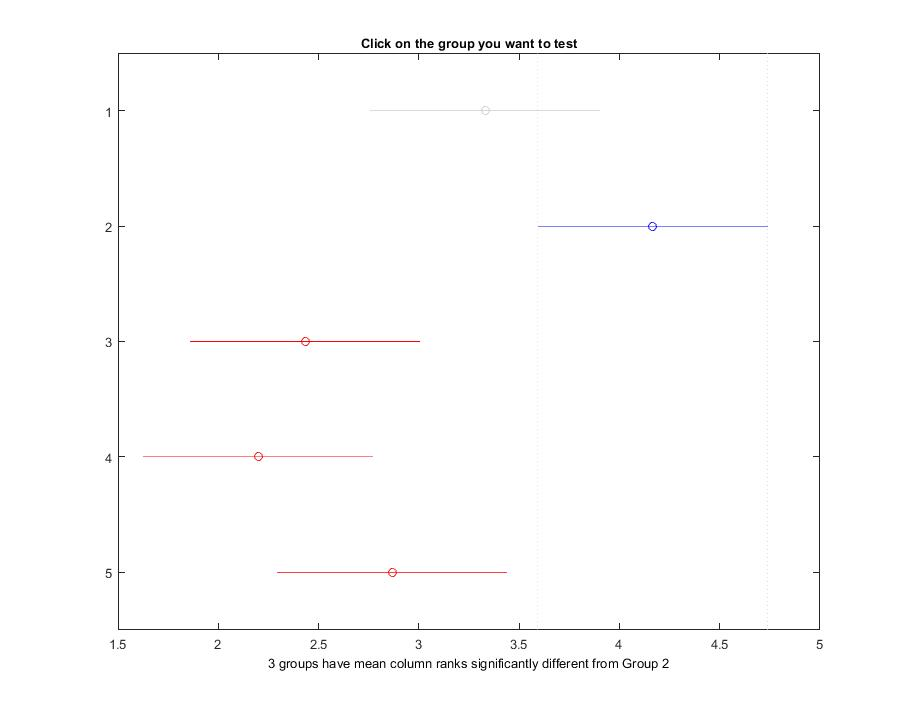
\includegraphics[width=\linewidth]{Figures/NMELA_FB_P1}
		\caption{MCE1} \label{fig:M1} 
	\end{subfigure}
	\begin{subfigure}[b]{0.49\linewidth}
		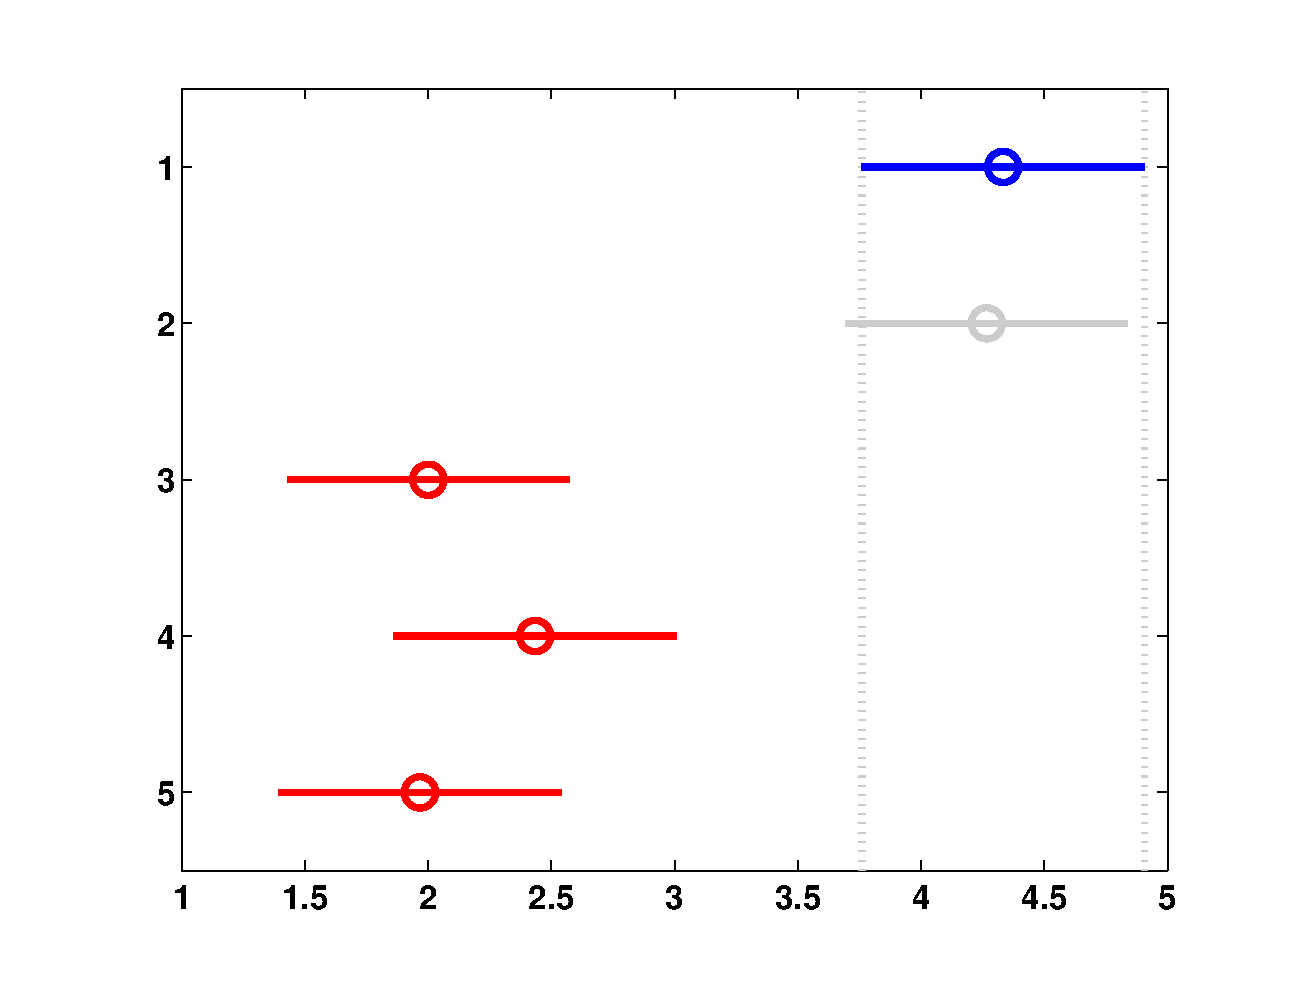
\includegraphics[width=\textwidth]{Figures/NMELA_FB_P2}
		\caption{MCE2} \label{fig:M2} 
	\end{subfigure}
	\begin{subfigure}[b]{0.49\linewidth}
		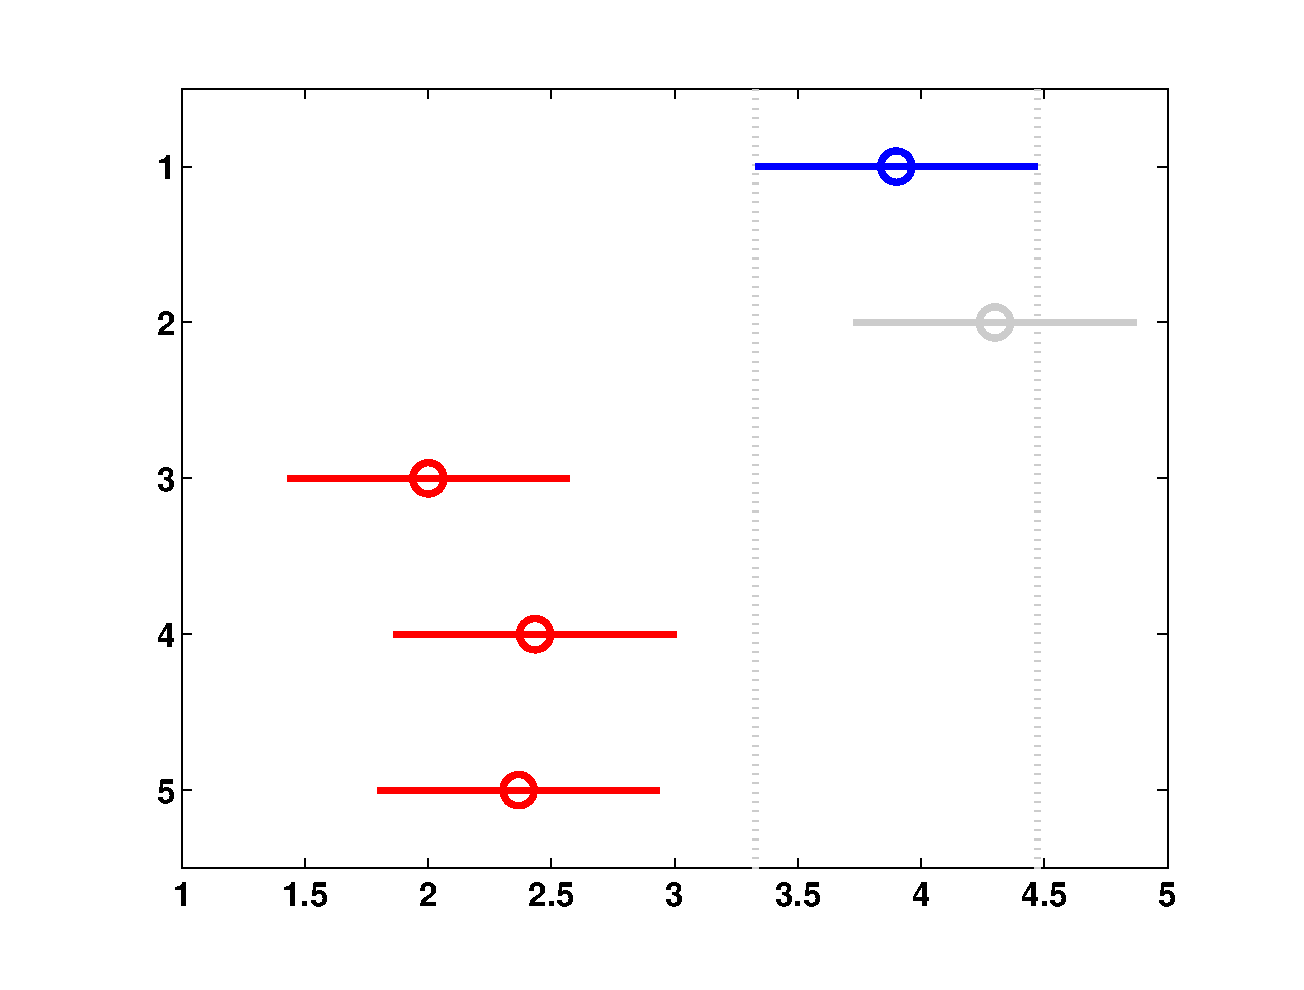
\includegraphics[width=\linewidth]{Figures/NMELA_FB_P3}
		\caption{MCE3} \label{fig:M3} 
	\end{subfigure}
	\begin{subfigure}[b]{0.49\linewidth}
		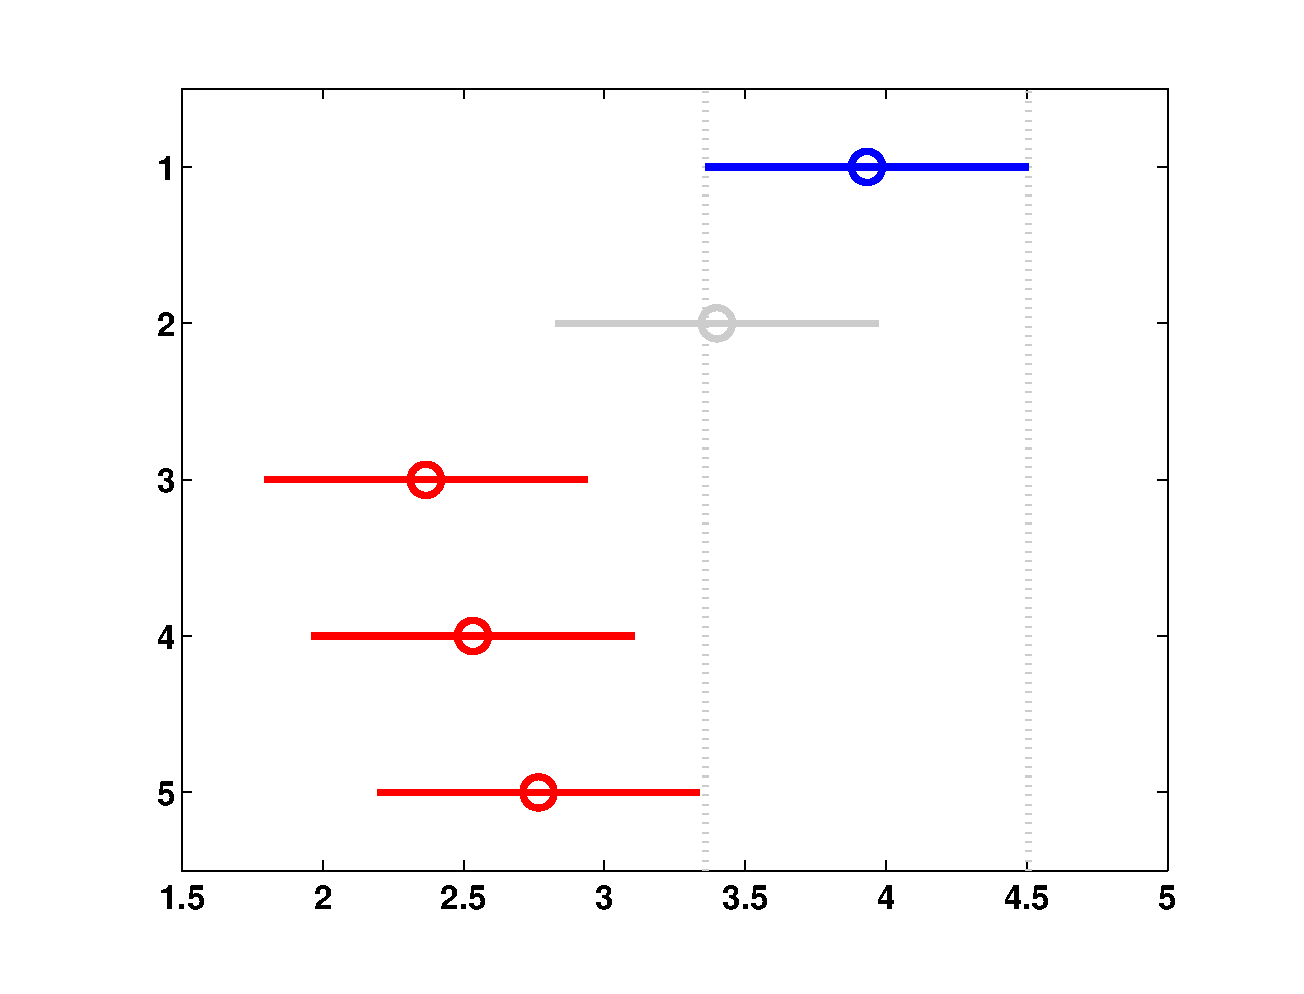
\includegraphics[width=\linewidth]{Figures/NMELA_FB_P4}
		\caption{GCE1} \label{fig:M4} 
	\end{subfigure}
	\begin{subfigure}[b]{0.49\linewidth}
		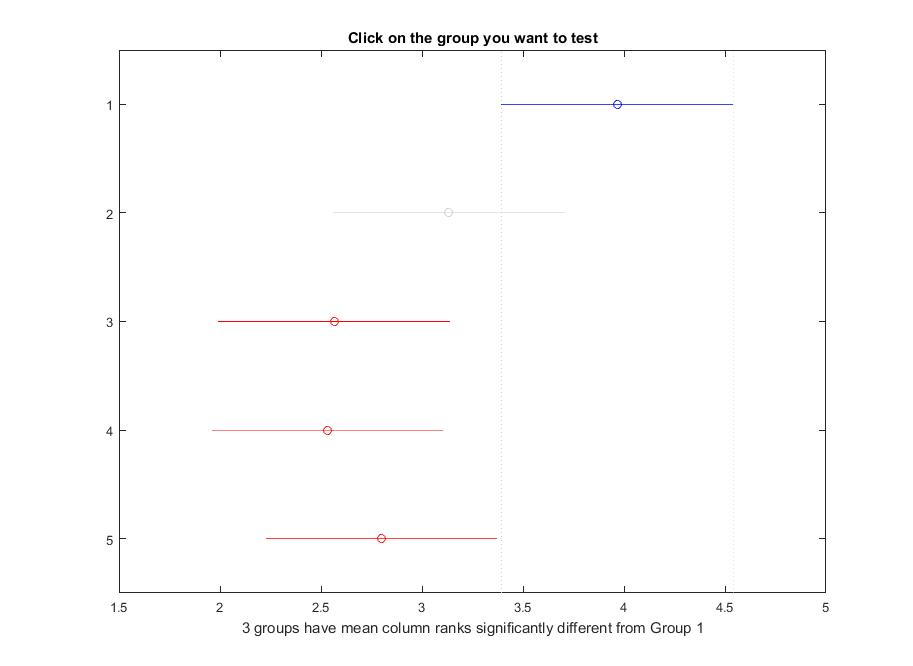
\includegraphics[width=\linewidth]{Figures/NMELA_FB_P5}
		\caption{GCE2} \label{fig:M4} 
	\end{subfigure}
	\caption[Resultados de las pruebas de Bonferroni-Dunn para las variantes NMELA y NM en Experimento A.]{Resultados de las pruebas de Bonferroni-Dunn para las variantes NMELA y NM en Experimento A. Se etiquetan en el eje vertical del 1 al 5 los algoritmos NM, NMS, NMELA, NMEILA, NM2ELA respectivamente.} \label{fig: Bonferroni-Dunn -NMELA} 
	
\end{figure}
\subsubsection{Observaciones}
En la Tabla \ref{tab:resultados NMELA} se pueden observar que las variantes NMLEA obtienen los mejores resultados en todas las medidas de estadística descriptiva y son capaces de acercase, igualar o superar en el mejor valor de la muestra a los mínimos encontrados para estos problemas. Sin embargo las medidas de tendencia central y dispersión  se encuentran lejos de estos mínimos en la mayoría de los problemas, lo que indica la sensibilidad de estos algoritmos a los puntos iniciales. El resultado de las pruebas de Friedman y Bonferroni-Dunn indican en  todos los problemas existen diferencias significativas entre al menos una variante determinista y una variante aleatorizada. Para los problemas MCE2 y MCE3 existen diferencias significativas entre el grupo determinista marcado en azul y las versiones propuestas que se encuentran a la izquierda en el grupo de color rojo con las mejores jerarquías. La capacidad del método Nelder-Mead para utilizar eficazmente información proveniente de regiones lejanas al área donde se encuentra operando, es la característica fundamental observada de forma experimental, por la cual se elige como método de búsqueda local para el diseño de los algoritmos híbridos HNMED. 



%%%%%%%%%%%%%%%%%%%%%%%%%%%%%%%%%%%%%%%%%%%%%%%%%%%%%%%%%%%%%%%%%%%%%%%%%%%%%%%%%%%%%%%%%%%%%%%%%%%%%%%%%%%%
\subsection{Experimento B: Comparación de desempeño entre Variantes HNMED vs ED/rand/1/bin}
El primer experimento se realiza para responder preguntas de investigación básicas sobre el enfoque de hibridación propuesto:
\begin{enumerate}
	\item ¿ Son los algoritmos diseñados de acuerdo al enfoque propuesto capaces de hallar valores iguales o cercanos a los mínimos conocidos para los problemas planteados ?
	\item ¿ Con qué frecuencia los algoritmos diseñados de acuerdo al enfoque propuesto son capaces de hallar valores iguales o cercanos a  los mínimos conocidos para los problemas planteados ?
	\item ¿ Con qué rapidez los algoritmos diseñados de acuerdo al enfoque propuesto son capaces converger a los mínimos conocidos para los problemas planteados ?
	\item ¿ Presentan los algoritmos propuestos en conjunto un desempeño significativamente mejor a la Evolución Diferencial en los problemas de optimización a resolver?
	\item ¿ Cuáles de los algoritmos propuestos presentan mejor desempeño?
\end{enumerate}
\subsubsection{Definición de medidas}
Se obtendrá para cada algoritmo una muestra de $n$ ejecuciones. Cada elemento de la muestra es el valor de la función objetivo del mejor individuo factible encontrado en la ejecución $i$ para $i= \{ 1,2,...,n\}$. Para cada muestra se obtendrá:
\begin{enumerate}
	\item \textbf{Mejor}: valor mínimo de función objetivo registrado en la muestra.
	\item \textbf{Peor}: valor máximo registrado en la muestra.
	\item \textbf{Mediana}: valor que se encuentra en el centro de la muestra ordenada. Esta medida es fundamental para evaluar el desempeño ya que el promedio puede ser afectado por valores anómalos. 
	\item \textbf{Promedio}: valor característico o tendencia central la muestra.
	\item \textbf{Desviación estándar}: grado de dispersión de las soluciones registradas en la muestra con respecto al promedio.
	\item \textbf{Gráfica de convergencia}: Presenta el valor de la función objetivo del mejor individuo en la población en cada evaluación para la ejecución correspondiente a la mediana de la muestra. La graficación de estos valores permite observar la rapidez de convergencia de los métodos.
    \item \textbf{Prueba de Friedman}: con nivel significancia $\alpha=0.05$ para determinar si existen diferencias significativas entre el desempeño de al menos dos de los algoritmos comparados. 
	\item \textbf{Prueba Bonferroni-Dunn}: con nivel significancia $\alpha=0.05$. Teniendo en cuenta el promedio jerarquías obtenidas en la prueba de Friedman se determina entre cuáles de los algoritmos comparados existe una diferencia significativa de desempeño.     
\end{enumerate}
\subsubsection{Planificación pre-experimental y configuración}
Para el presente experimento se generaron 6 muestras correspondientes a las 5 variantes propuestas y la  ED/rand/1/bin de tamaño $n=31$. Las ejecuciones se llevaron a cabo en una computadora con procesador AMD Athlon II X2, memoria RAM 2GB, sistema operativo Windows 7 con arquitectura de 64 bits y como entorno de programación se utilizó  MatLab R2016b. 

Para este experimento se utilizó un número fijo de evaluaciones (las utilizadas por la ED) para todos los algoritmos en comparación en cada problema de optimización según se describe en la tabla \ref{tab:Evaluaciones utilizadas por problema de optimización: Experimento B.}:

\begin{table}[]
	\centering
	\caption{Evaluaciones utilizadas por problema de optimización: Experimento B.}
	\label{tab:Evaluaciones utilizadas por problema de optimización: Experimento B.}
	\begin{tabular}{cc}
		\textbf{Problema} &   \textbf{Evaluaciones}     \\
		\hline
		MCE1   &   750030       \\
		MCE2   &   20000       \\
		MCE3   &   450018      \\
		GCE1   &   750030       \\
		GCE2   &   750030      \\
		SCE1   &   288000       \\
	\end{tabular}
\end{table}
La configuración de parámetros utilizada por las variantes HNMED y la ED es la siguiente:
\begin{enumerate}
	\item Se establece la probabilidad de cruza $CR=\{0.8, 1\}$ para ED y HNMED para todos los problemas.
	\item Se establece el factor de escala $F=\{0.3, 0.9\}$ para ED y HNMED para todos los problemas.
	\item Para las variantes HNMED se establecieron los parámetros de reflexión $\alpha=2$, expansión $\gamma=1.5$ $\beta=0.5$ para todos los problemas.
	\item El tamaño de población se estableció según la Tabla \ref{tab:Tamaño de población utilizados para cada problema en el experimento B.}. Donde el valor $NS$ se refiere a la cantidad de símpleces utilizados los cuales determinan la población para cada problema $NP=NS(N+1)$ donde $N$  es la dimensión del problema.
\end{enumerate}

\begin{table}[]
	\centering
	\caption{Tamaño de población utilizados para cada problema en el experimento B.}
	\label{tab:Tamaño de población utilizados para cada problema en el experimento B.}
	\begin{tabular}{cccc}
		& \textbf{ED/rand/1/bin }& \multicolumn{2}{l}{\textbf{HNMED}} \\
		\hline
		\textbf{Problema} & \textbf{NP}            & \textbf{NS}          & \textbf{NP}          \\
		\hline
		MCE1     & 138           & 9           & 144         \\
		MCE2     & 50            & 4           & 28          \\
		MCE3     & 138           & 7           & 140         \\
		GCE1     & 138           & 9           & 135         \\
		GCE2     & 138           & 8           & 135         \\
		SCE1     & 50            & 7           & 35         
	\end{tabular}
\end{table}

\subsubsection{Presentación de resultados}
En la Tabla \ref{tab:Resultados estadísticos obtenidos por variantes HNMED y DE/rand/1/bin  experimento B.} se muestran los resultados obtenidos en la estadísticas descriptivas para las variantes propuestas y la ED/rand/1/bin en los 6 problemas de optimización. Los resultados ganadores se resaltan en letra negrita. A pesar de que existe el análisis teórico para determinar la velocidad de convergencia, los experimentos realizados se limitaron a la graficación del valor de $f(x)$ presentado por el mejor individuo factible en la población, en función del número de evaluaciones de $f(x)$ denominado $NEF$. En la Figura \ref{fig: Gráficas de convergencia para las variantes HNMED y ED/rand/1/bin} se muestran las gráficas de convergencia de la ejecución correspondiente a la mediana de la muestra. En caso del problema de la micro-red eléctrica Se grafican los valores de función objetivo correspondientes a la hora 12.   

\begin{table}
	
	\caption[Resultados estadísticos obtenidos por las variantes HNMED y DE/rand/1/bin en el Experimento B para los seis problemas de optimización.]{Resultados estadísticos obtenidos por las variantes HNMED y DE/rand/1/bin en el Experimento B para los seis problemas de optimización. Se marcan en negritas los mejores valores de cada medida.}\label{tab:Resultados estadísticos obtenidos por variantes HNMED y DE/rand/1/bin  experimento B.}
	
	\centering
	\resizebox{\textwidth}{!}{%
		\begin{tabular}{clcccccc} 
			\hline
			Problema              & Estadística   & HNMED-V1 & HNMED-V2 &HNMED-V3 &HNMED-V4 &HNMED-V5 & ED/rand/1/bin  \\ 
			\hline
			\multirow{6}{*}{MCE1} & Mejor        & 5.55358E-28 &5.31513E-07& \textbf{0} & 1.26218E-29&5.04871E-29 &1.7670E-28 \\
			& Peor        & 2.73815E-02 & 1.6149E+00 & 2.5685E-02 & \textbf{2.2528E-02} & 2.5749E-02 & 2.7649E-02 \\
			& Mediana     & 2.2312E-04 & 2.5478E-04  & 2.0521E-04 & 2.4414E-04 & 2.1680E-04 & \textbf{4.2746E-06 }  \\
			& Promedio    & 2.6670E-03 & 5.4682E-02  & \textbf{1.8612E-03} & 3.6684E-03 & 2.5208E-03 & 2.9850E-01  \\
			& Desv. Est.   & 7.3917E-03 & 2.8965E-01 &\textbf{ 6.2715E-03} & 7.9230E-03 & 7.1453E-03 & 8.1906E-03  \\
			\hline                      
			\multirow{6}{*}{MCE2} & Mejor        &  2.6280E-03 & 2.6280E-03 &  2.6280E-03 &  2.6280E-03 &  2.6280E-03 & 2.6280E-03 \\
			& Peor        & 2.6290E-03 &  \textbf{2.6280E-03}  &  \textbf{2.6280E-03} &  \textbf{2.6280E-03}&  \textbf{2.6280E-03 }& 2.6426E-03 \\
			& Mediana     &2.6280E-03 &  2.6280E-03 &  2.6280E-03&  2.6280E-03 & 2.6280E-03 & 2.6280E-03\\
			& Promedio    & 2.6281E-03 &\textbf{2.6280E-03 }& \textbf{ 2.6280E-03} & \textbf{2.6280E-03} &  \textbf{2.6280E-03} & 2.6288E-03 \\
			& Desv. Est.   &2.3345E-07 &\textbf{ 17600E-18}  &1.0776E-15&  3.2328E-15 &  \textbf{1.7600E-18 }& 2.7205E-06\\   
			\hline
			
			\multirow{6}{*}{MCE3} & Mejor       & 2.7496E-01 & 2.7496E-01 & 2.7496E-01 & 2.7496E-01 &  2.7496E-01 & 2.7496E-01 \\
			& Peor        & 1.3508E+01 & 1.3508E+01 & 1.3508E+01 & 1.3508E+01& 1.3508E+01 &  1.3508E+01 \\
			& Mediana     & 4.3436E-01  & 1.6290E+00& 9.1663E-01 & 6.6851E-01& 4.2346E-01 &\textbf{2.7563E-01} \\
			& Promedio    & 4.2838E+00 &  6.4180E+00& 4.7519E+00 & 5.1492E+00 & 5.5448E+00 & \textbf{1.2313E+00} \\
			& Desv. Est.  & 6.0160E+00  & 6.5415E+00& 5.9814E+00 & 6.3172E+00 & 6.4445E+00  &\textbf{3.2919E+00}\\
			\hline
			\multirow{6}{*}{GCE1} & Mejor        &2.8398E-29 & \textbf{0}          & \textbf{0}          &\textbf{0}           & \textbf{0}          &6.7147E-27 \\
			& Peor        & 3.1333E-27 & 1.7670E-27 & 6.8157E-28 & 6.3109E-29 &\textbf{5.0487E-29} & 5.9926E-20\\
			& Mediana     & 1.0302E-28 & 3.1554E-30 & 3.1554E-30 & 1.5777E-30 & \textbf{0}& 3.9485E-23 \\
			& Promedio    & 1.2272E-27 & 8.7721E-29  & 4.3439E-29 &1.1359E-29 & \textbf{7.9937E-30 }& 3.4957E-21 \\
			& Desv. Est.  & 97794E-28 & 3.2234E-28  & 1.2753E-28 & \textbf{1.6873E-29 }& 1.7728E-29  & 1.2077E-20\\
			\hline
			
			\multirow{6}{*}{GCE2} & Mejor        & \textbf{1.1385E-01 }& \textbf{1.1385E-01}  & \textbf{1.1385E-01 }& \textbf{1.1385E-01}& \textbf{1.1385E-01} & 1.1388E-01 \\
			& Peor        & 1.9561E-01 & 1.5875E-01  & 1.5965E-01& 1.5976E-01 & \textbf{1.5751E-01} & 1.6075E-01\\
			& Mediana     & 1.1995E-01& 1.1440E-01  & 1.5199E-01 & 1.1410E-01 & \textbf{1.1385E-01} & 1.1447E-01 \\
			& Promedio    & 1.3600E-01& 1.3166E-01  & 1.3561E-01 & 1.2979E-01 & 1.2940E01 & \textbf{1.2080E-01} \\
			& Desv. Est.   &2.4766E-02 & 2.0980E-02  & 2.1283E-02 & 1.9838E-01& 1.9926E-02 & \textbf{1.4713E-02} \\
			\hline                      
			\multirow{6}{*}{SCE1} & Mejor        & -5.7049E+05&	\textbf{-5.7741E+05}&	-5.6195E+05&	-5.4519E+05&-5.3238E+05 &-5.3206E+05 \\
			& Peor        & -5.1016E+05&	-5.2146E+05&	-5.2772E+05&	-5.3071E+05&	\textbf{-5.3198E+05} &-5.3204E+05 \\
			& Mediana     & -5.3059E+05&	-5.3158E+05&	-5.3135E+05&	-5.3184E+05&	\textbf{-5.3209E+05 }& -5.3205E+05 \\
			& Promedio    & -5.3174E+05&	\textbf{-5.3339E+05}&	-5.3308E+05&	-5.3236E+05&	-5.3214E+05& -5.3205E+05\\
			& Desv. Est.   & 1.1452E+04&	9.2013E+03&	7.1985E+03&	2.4432E+03&	1.0096E+02& \textbf{3.3010E+00}\\
			\hline
			
			
			
			
			
			
			
		\end{tabular}
	}
\end{table}

%Grafica_Convergencia_Problema

\begin{figure}
	\centering
	\begin{subfigure}[b]{0.49\linewidth}
		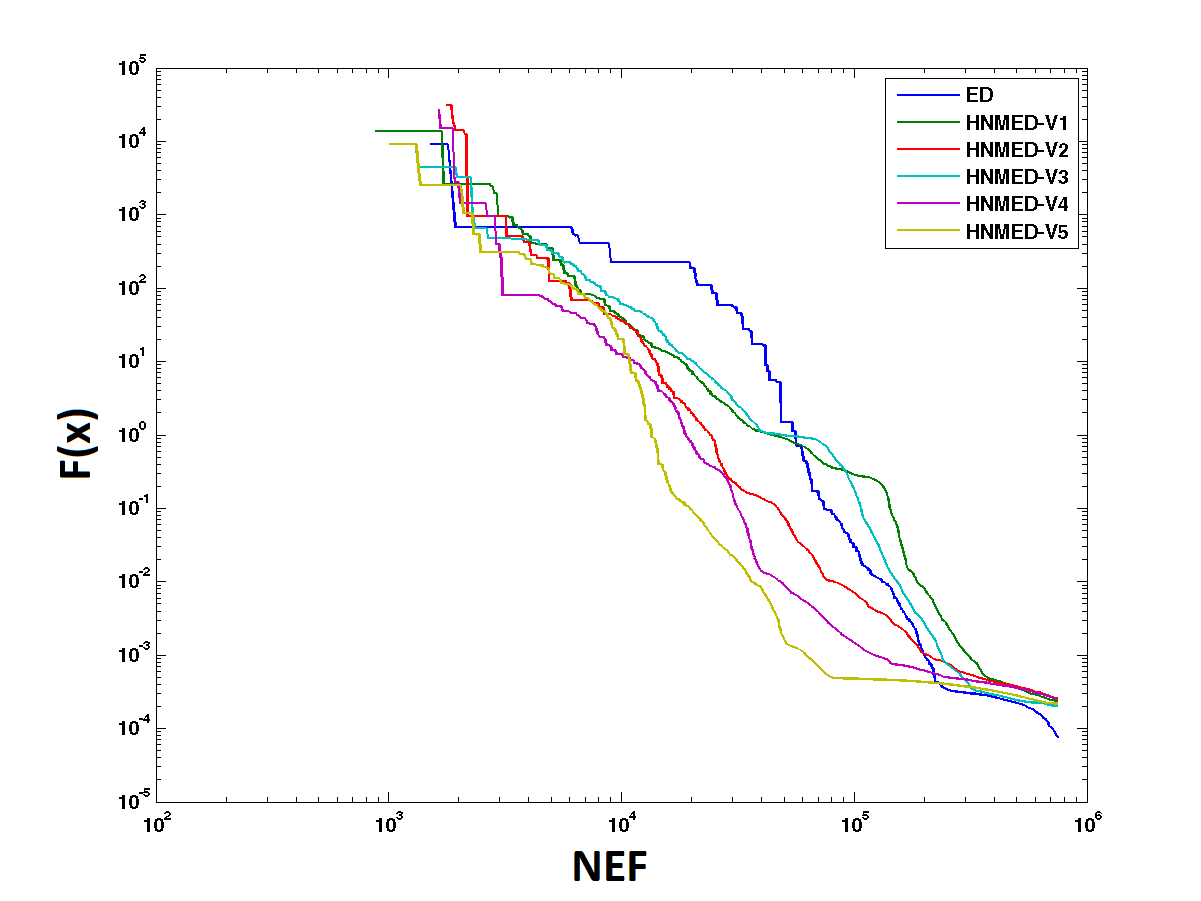
\includegraphics[width=\linewidth]{Figures/B-Grafica_Convergencia_Problema_1}
		\caption{MCE1} \label{fig:M1} 
	\end{subfigure}
	\begin{subfigure}[b]{0.49\linewidth}
		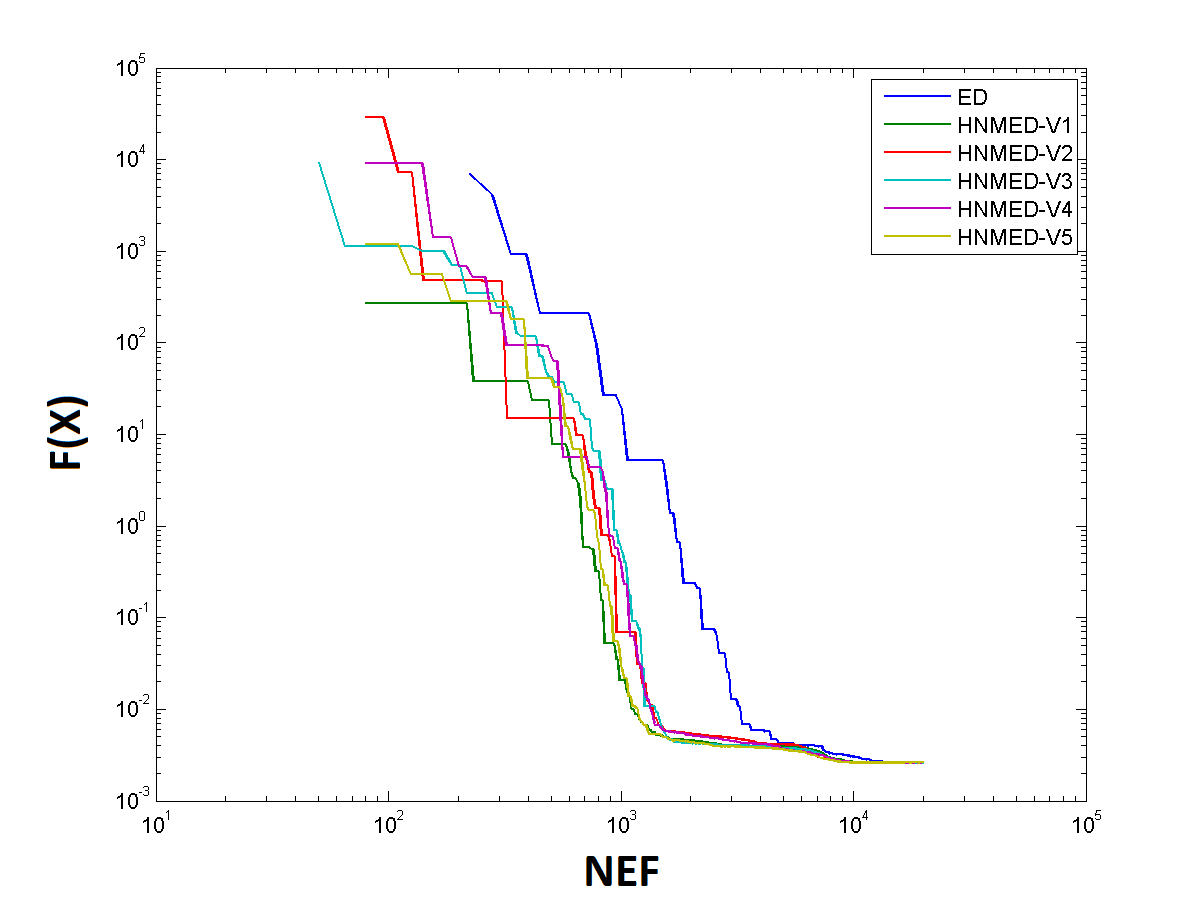
\includegraphics[width=\textwidth]{Figures/B-Grafica_Convergencia_Problema_2}
		\caption{MCE2} \label{fig:M2} 
	\end{subfigure}
	\begin{subfigure}[b]{0.49\linewidth}
		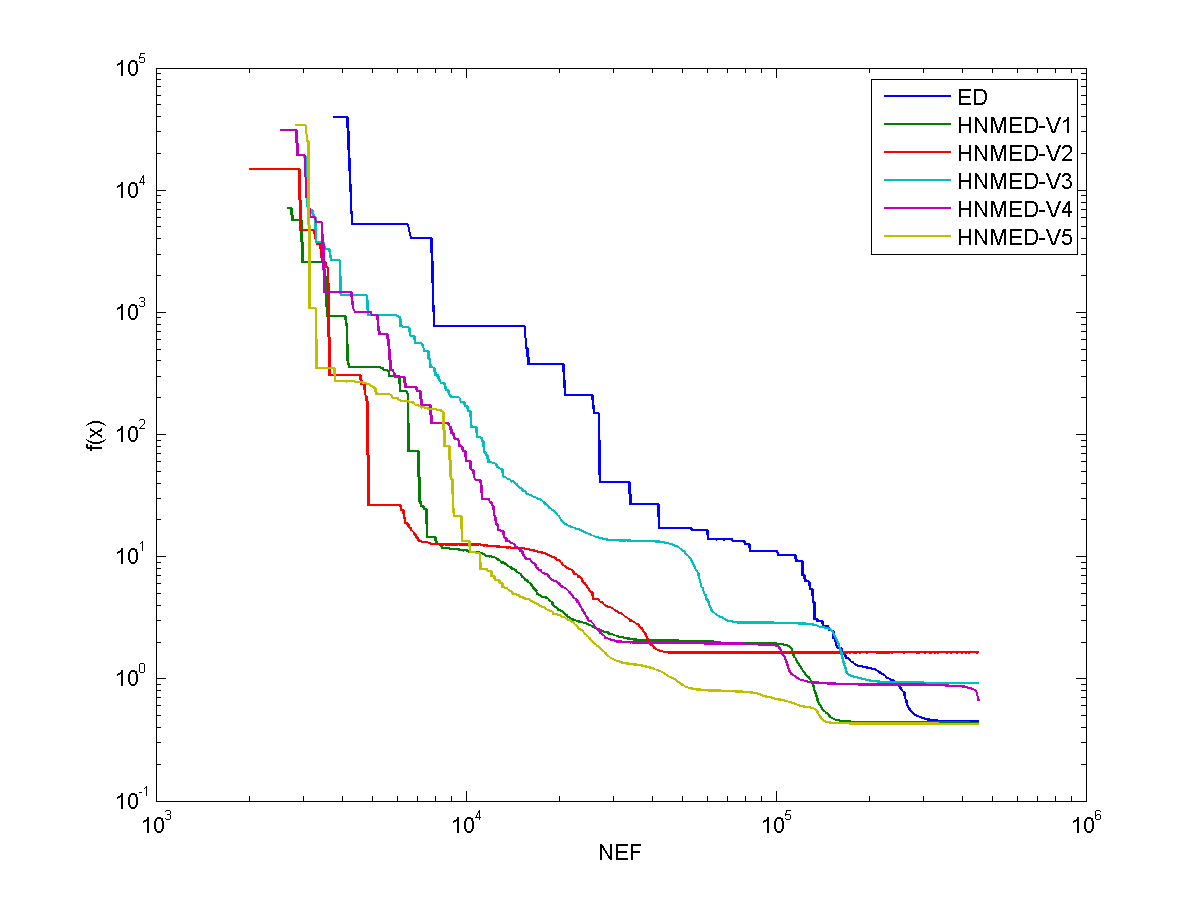
\includegraphics[width=\linewidth]{Figures/B-Grafica_Convergencia_Problema_3}
		\caption{MCE3} \label{fig:M3} 
	\end{subfigure}
	\begin{subfigure}[b]{0.49\linewidth}
		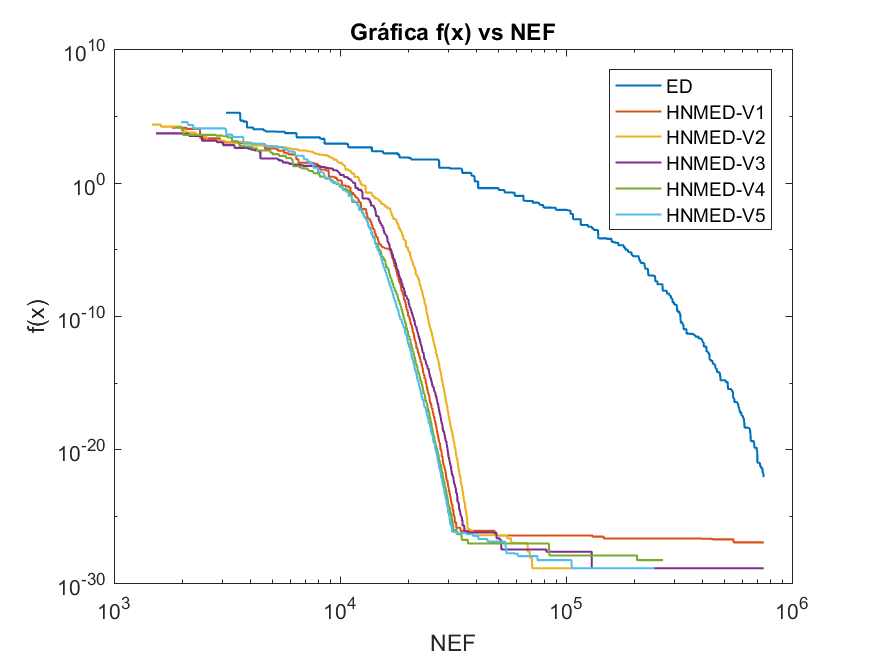
\includegraphics[width=\linewidth]{Figures/B-Grafica_Convergencia_Problema_4}
		\caption{GCE1} \label{fig:G1} 
	\end{subfigure}
	\begin{subfigure}[b]{0.49\linewidth}
		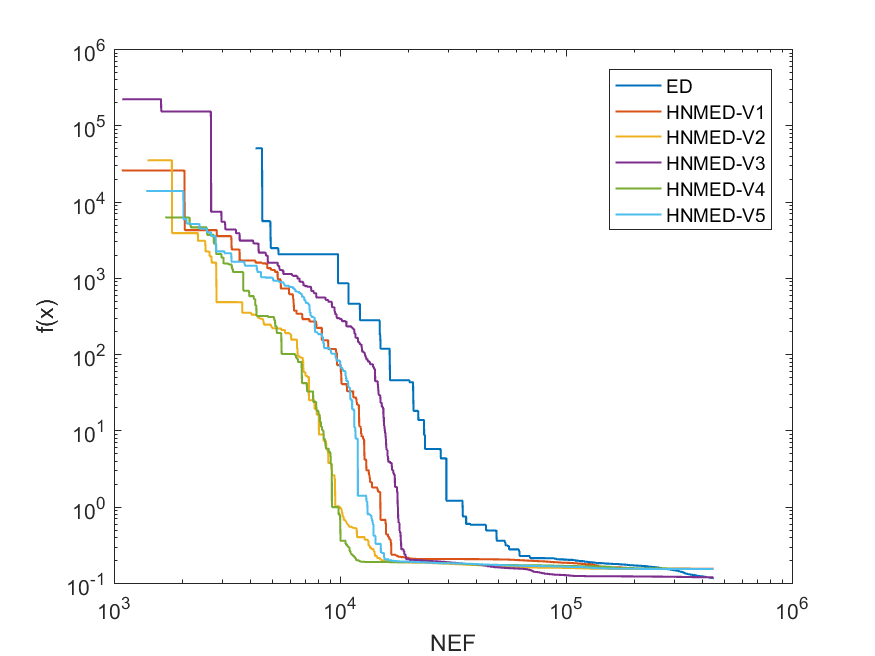
\includegraphics[width=\linewidth]{Figures/B-Grafica_Convergencia_Problema_5}
		\caption{GCE2} \label{fig:G2} 
	\end{subfigure}
	\begin{subfigure}[b]{0.49\linewidth}
		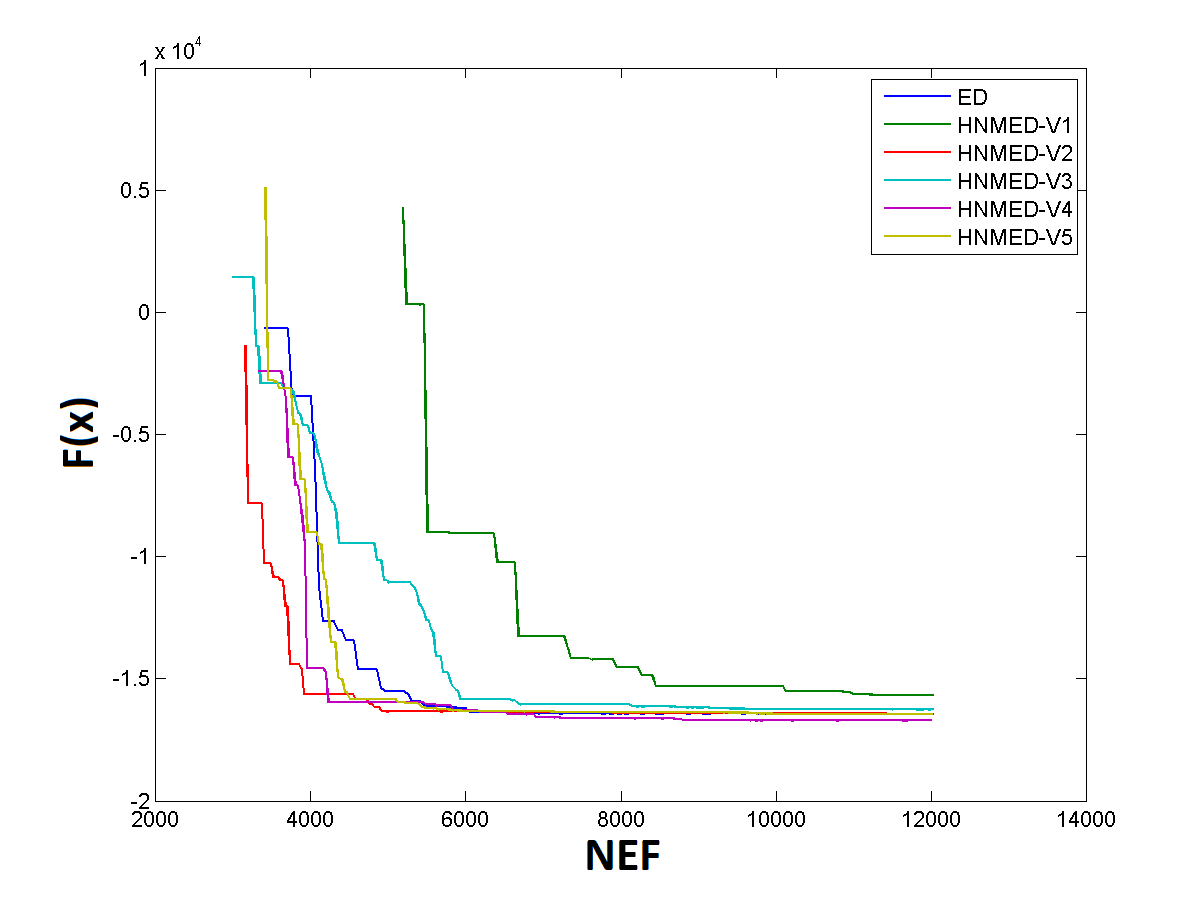
\includegraphics[width=\linewidth]{Figures/B-Grafica_Convergencia_Problema_6}
		\caption{SCE2} \label{fig:S1} 
	\end{subfigure}
	\caption[Gráficas de convergencia obtenidas por las variantes HNMED y ED/rand/1/bin en el Experimento B.]{Gráficas de convergencia obtenidas por las variantes HNMED y ED/rand/1/bin en el Experimento B. El eje horizontal presenta el número de evaluaciones de la función objetivo (NEF) y el eje vertical el valor de  $f(x)$.  } \label{fig: Gráficas de convergencia para las variantes HNMED y ED/rand/1/bin} 
	
\end{figure}
En la Tabla \ref{tab:Resultados Firedman obtenidos por variantes HNMED y DE/rand/1/bin  experimento B.} se presentan las jerarquías promedios obtenidas por los algoritmos, los valores $p$ y la aceptación o rechazo de la hipótesis obtenidas en la prueba de Firedman en cada uno de los problemas de optimización. Se resaltan en letra negrita las promedios de jerarquías ganadores.

Teniendo en cuenta los resultados de la prueba de Friedman, la Figura \ref{fig: Resultados de las pruebas de Bonferroni-Dunn para las variantes HNMED vs ED/rand/1/bin en el Experitmento B} la prueba post hoc de Bonferroni-Dunn para los 6 problemas. En las gráficas, el eje vertical presenta las etiquetas dadas a cada algoritmo y el horizontal las jerarquías promedios. Las etiquetas están asignadas de la siguiente forma: a la ED le corresponde el número 1 y a las variantes HNMED desde V1 a V5 les corresponden los números del 2 al 6 respectivamente. Los círculos corresponden a la asignación de la etiqueta $L_j$ con el promedio jerarquía  $R_j$. Las lineas son los intervalos de confianza calculados por la prueba. 

Cuando los intervalos de confianza de dos muestras no se traslapan, se rechaza la sub-hipótesis nula y por lo tanto se afirma que existen diferencias significativas entre los algoritmos que describen dichas muestras. En las figuras presentadas los promedios de jerarquía e intervalos de confianza entre los cuales existen diferencias significativas se dibujan con colores diferentes (azul y rojo) para hacer más legible la gráfica.     
%%%%%%%%%%%%%%%%%%%%%%

\begin{table}
	\centering
	\caption[Resultados de la prueba de Friedman obtenidos por las variantes HNMED y DE/rand/1/bin en el Experimento B para los seis problemas de diseño mecatrónico.]{Resultados de la prueba de Friedman obtenidos por las variantes HNMED y DE/rand/1/bin en el Experimento B para los seis problemas de diseño mecatrónico. Se resaltan en negrita los promedios de jerarquía ganadores.}
	\label{tab:Resultados Firedman obtenidos por variantes HNMED y DE/rand/1/bin  experimento B.}
	\resizebox{\textwidth}{!}{%{0.3132\textheight}{%
		\begin{tabular}{lccccc}
			\hline
			Problema              & Algoritmo     & Jerarquía promedio &Valor de $p$        & $H_0$                           & $H_1$             \\
			\hline  
			\multirow{6}{*}{MCE1} & HNMED-V1      &3.6451E+00          &\multirow{6}{*}{8.1173E-01}  & \multirow{6}{*}{Aceptada}& \multirow{6}{*}{Rechazada} \\
			& HNMED-V2      &  3.8709E+00        &                    &                          &                            \\
			& HNMED-V3      &  3.3870E+00        &                    &                          &                            \\
			& HNMED-V4      &  3.4516E+00        &                    &                          &                            \\
			& HNMED-V5      &  3.4193E+00        &                    &                          &                            \\
			& ED/rand/1/bin &\textbf{3.2258E+00} &                    &                          &                            \\
			\hline  
			\multirow{6}{*}{MCE2} & HNMED-V1      & 3.5322E+00         & \multirow{6}{*}{1.3277E-26} & \multirow{6}{*}{Rechazada}& \multirow{6}{*}{Aceptada} \\
			& HNMED-V2      &\textbf{2.8387E+00 }&                    &                          &                            \\
			& HNMED-V3      & 2.9193E+00         &                    &                          &                            \\
			& HNMED-V4      & 2.9032E+00         &                    &                          &                            \\
			& HNMED-V5      &\textbf{2.8387E+00 }&                    &                          &                            \\
			& ED/rand/1/bin &   5.9677E+00       &                    &                          &                            \\
			\hline
			
			\multirow{6}{*}{MCE3} & HNMED-V1      &  3.5161E+00        & \multirow{6}{*}{9.4985E-01}  & \multirow{6}{*}{Aceptada}& \multirow{6}{*}{Rechazada} \\
			& HNMED-V2      & 3.7258E+00         &                    &                          &                            \\
			& HNMED-V3      & 3.5483E+00         &                    &                          &                            \\
			& HNMED-V4      & 3.5483E+00         &                    &                          &                            \\
			& HNMED-V5      &  3.5800E+00         &                    &                          &                            \\
			& ED/rand/1/bin & \textbf{3.2258E+00}    &                    &                          &                            \\
			\hline  
			\multirow{6}{*}{GCE1} & HNMED-V1      &   4.9000E+00       & \multirow{6}{*}{1.3365E-22}  & \multirow{6}{*}{Rechazada}& \multirow{6}{*}{Aceptada} \\
			& HNMED-V2      &   2.7333E+00       &                    &                          &                            \\
			& HNMED-V3      &   2.7333E+00       &                    &                          &                            \\
			& HNMED-V4      &   2.5000E+00       &                    &                          &                            \\
			& HNMED-V5      &\textbf{2.1333E+00} &                    &                          &                            \\
			& ED/rand/1/bin &   6.0000E+00       &                    &                          &                            \\
			\hline  
			\multirow{6}{*}{GCE2} & HNMED-V1      &  4.0967E+00        & \multirow{6}{*}{1.0989E-01}  & \multirow{6}{*}{Aceptada}& \multirow{6}{*}{Rechazada} \\
			& HNMED-V2      &  3.4032E+00        &                    &                          &                            \\
			& HNMED-V3      &  3.8387E+00        &                    &                          &                            \\
			& HNMED-V4      &  3.0483E+00        &                    &                          &                            \\
			& HNMED-V5      & \textbf{2.9677E+00}      &                    &                          &                            \\
			& ED/rand/1/bin & 3.0322E+00&                    &                          &                            \\
			\hline  
			
			\multirow{6}{*}{SCE1} & HNMED-V1      & 3.8709E+00                   & \multirow{6}{*}{ 1.7205E-03 }  & \multirow{6}{*}{Rechazada}& \multirow{6}{*}{Aceptada} \\
			& HNMED-V2      & 3.7741E+00                   &                    &                          &                            \\
			& HNMED-V3      & 4.3225E+00                   &                    &                          &                            \\
			& HNMED-V4      & 3.4516E+00                   &                    &                          &                            \\
			& HNMED-V5      & \textbf{2.4193E+00 }         &                    &                          &                            \\
			& ED/rand/1/bin &3.1612E+00 &                  &                    &                            \\
			
		\end{tabular}
	}
\end{table}

% Pruebas de Bunferroni

\begin{figure}
	\centering
	\begin{subfigure}[b]{0.49\linewidth}
		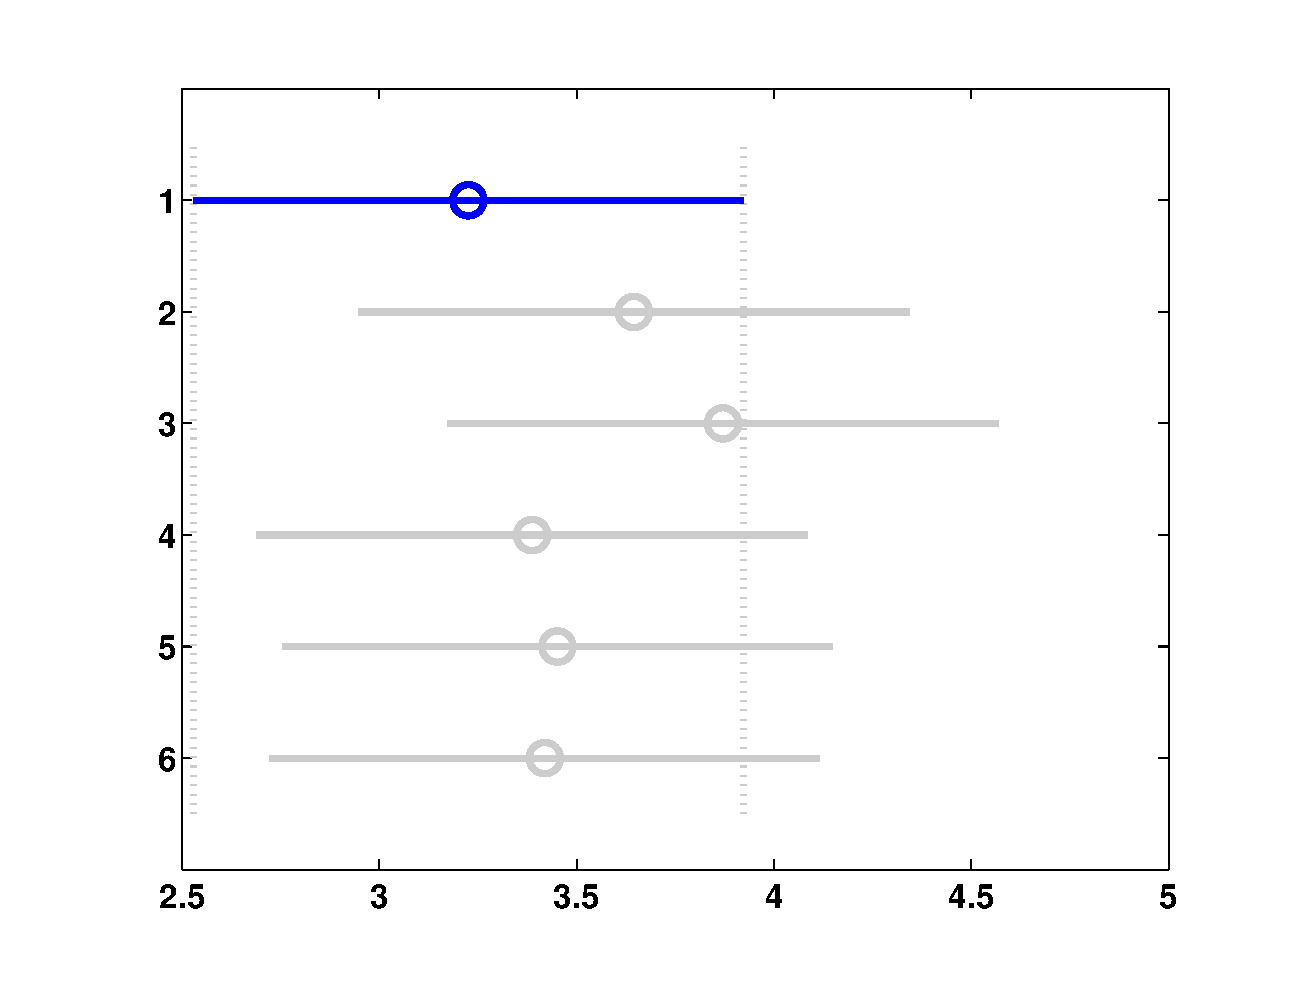
\includegraphics[width=\linewidth]{Figures/B-Bonferroni_HNMED_VS_ED1}
		\caption{MCE1} \label{fig:Bon_M1} 
	\end{subfigure}
	\begin{subfigure}[b]{0.49\linewidth}
		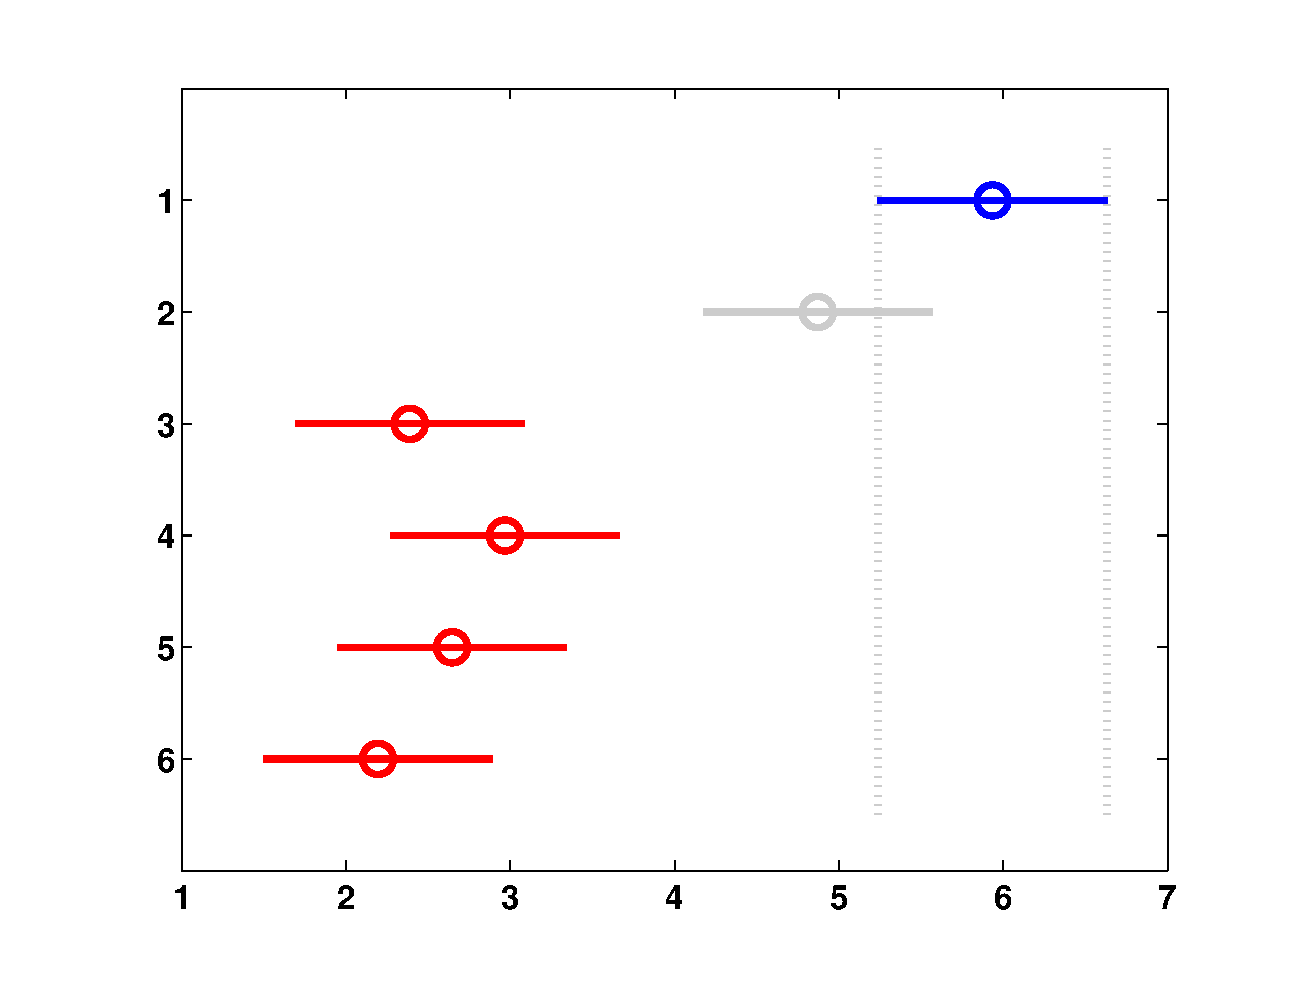
\includegraphics[width=\textwidth]{Figures/B-Bonferroni_HNMED_VS_ED2}
		\caption{MCE2} \label{fig:Bon_M2} 
	\end{subfigure}
	\begin{subfigure}[b]{0.49\linewidth}
		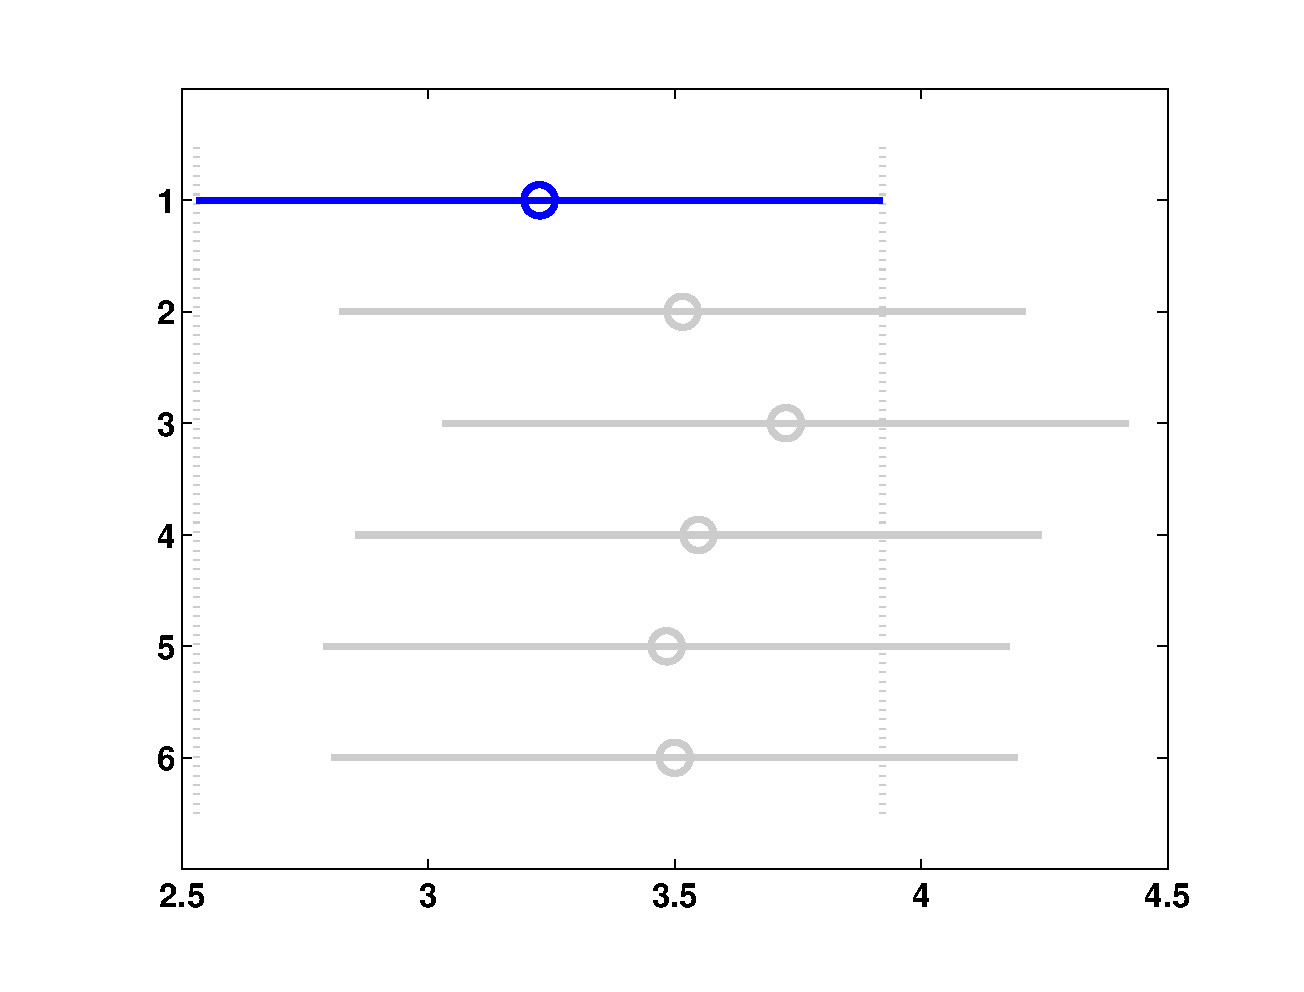
\includegraphics[width=\linewidth]{Figures/B-Bonferroni_HNMED_VS_ED3}
		\caption{MCE3} \label{fig:Bon_M3} 
	\end{subfigure}
	\begin{subfigure}[b]{0.49\linewidth}
		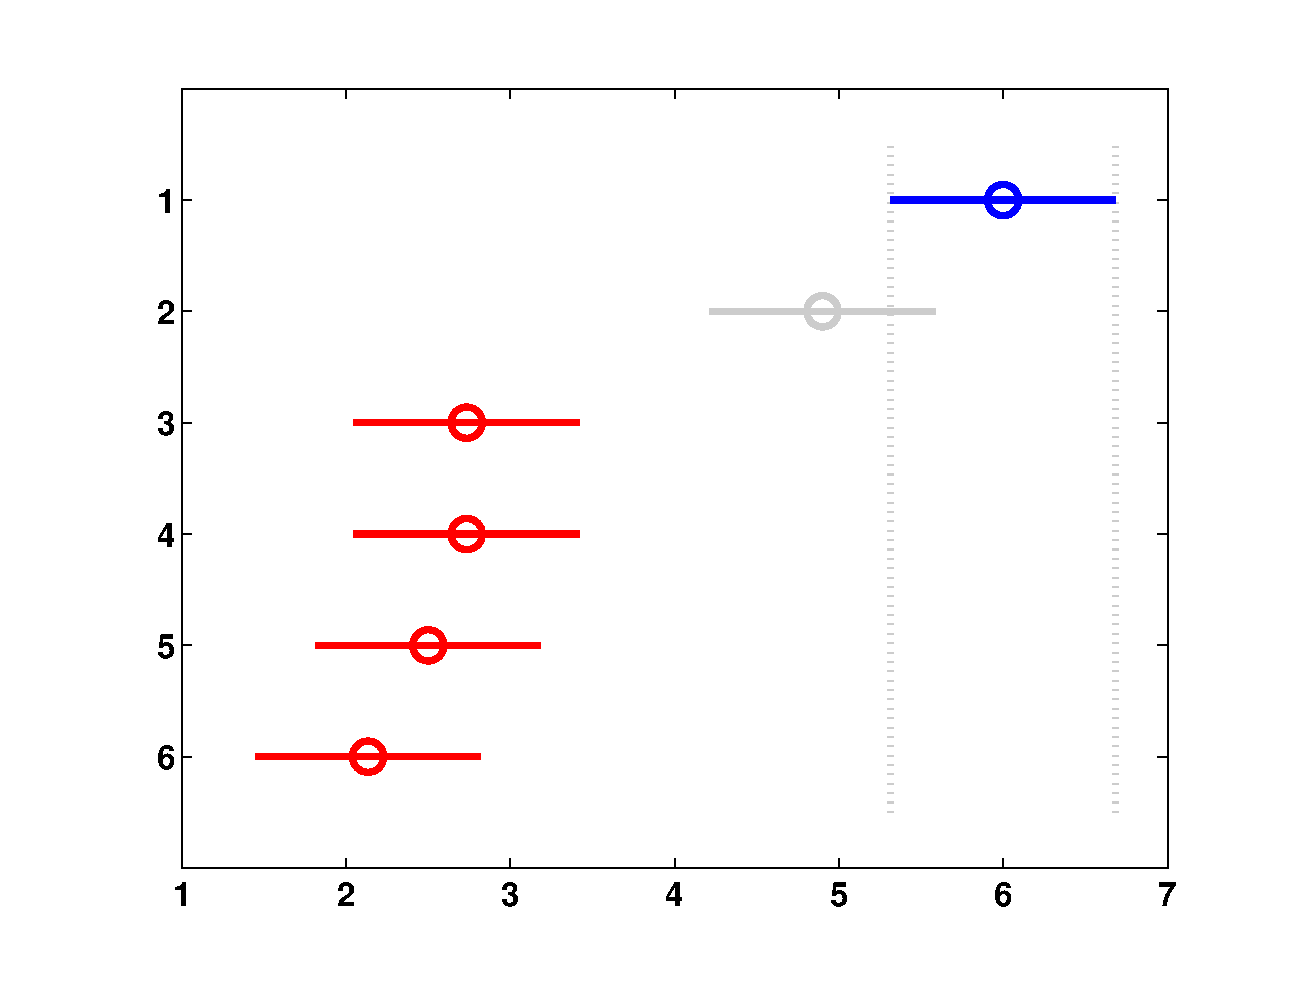
\includegraphics[width=\linewidth]{Figures/B-Bonferroni_HNMED_VS_ED4}
		\caption{GCE1} \label{fig:Bon_G1} 
	\end{subfigure}
	\begin{subfigure}[b]{0.49\linewidth}
		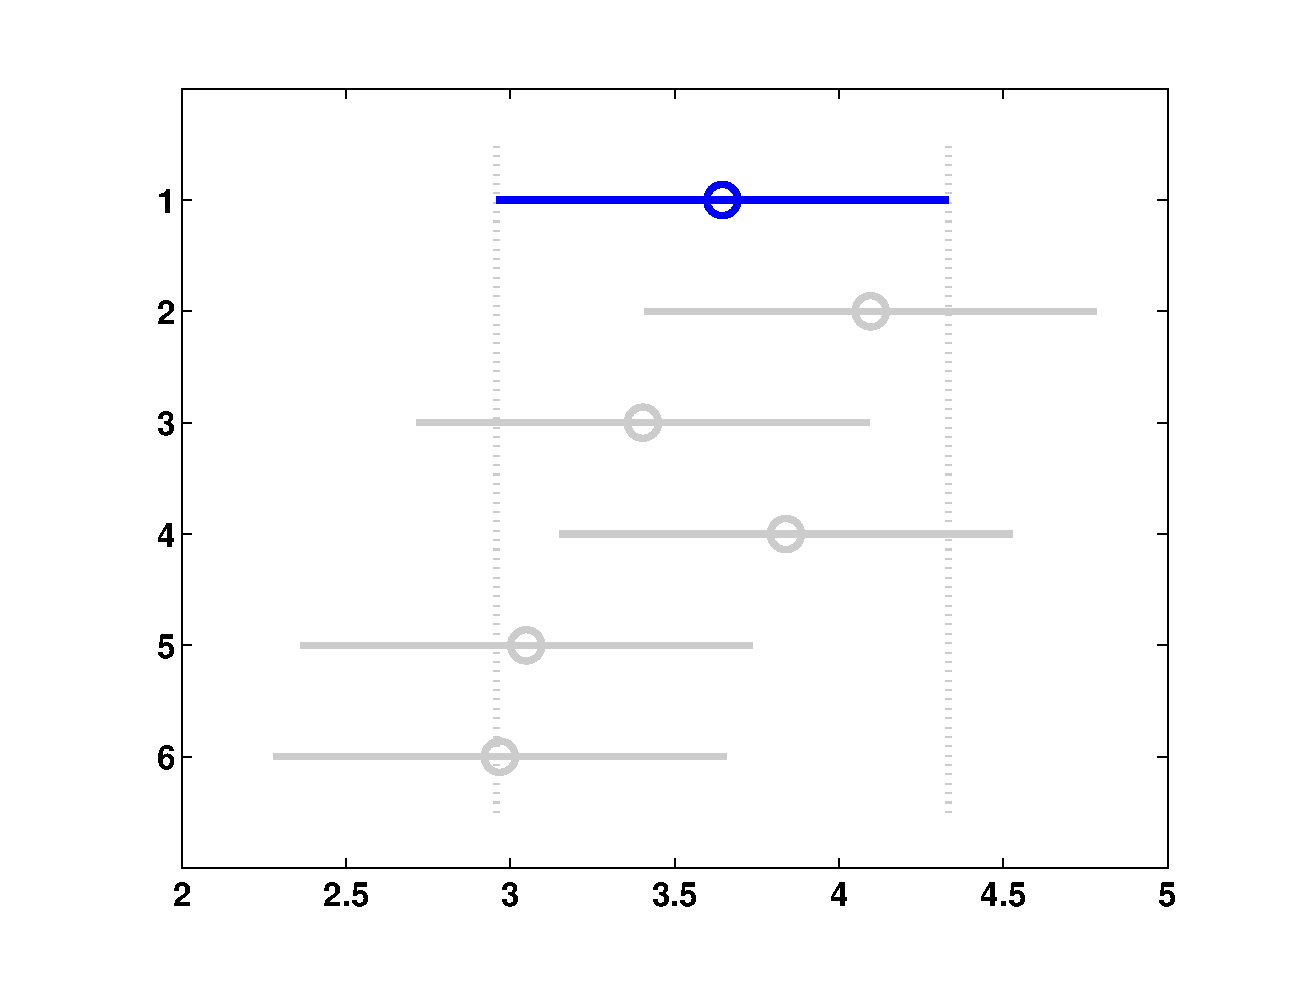
\includegraphics[width=\linewidth]{Figures/B-Bonferroni_HNMED_VS_ED5}
		\caption{GCE2} \label{fig:Bon_G2} 
	\end{subfigure}
	\begin{subfigure}[b]{0.49\linewidth}
		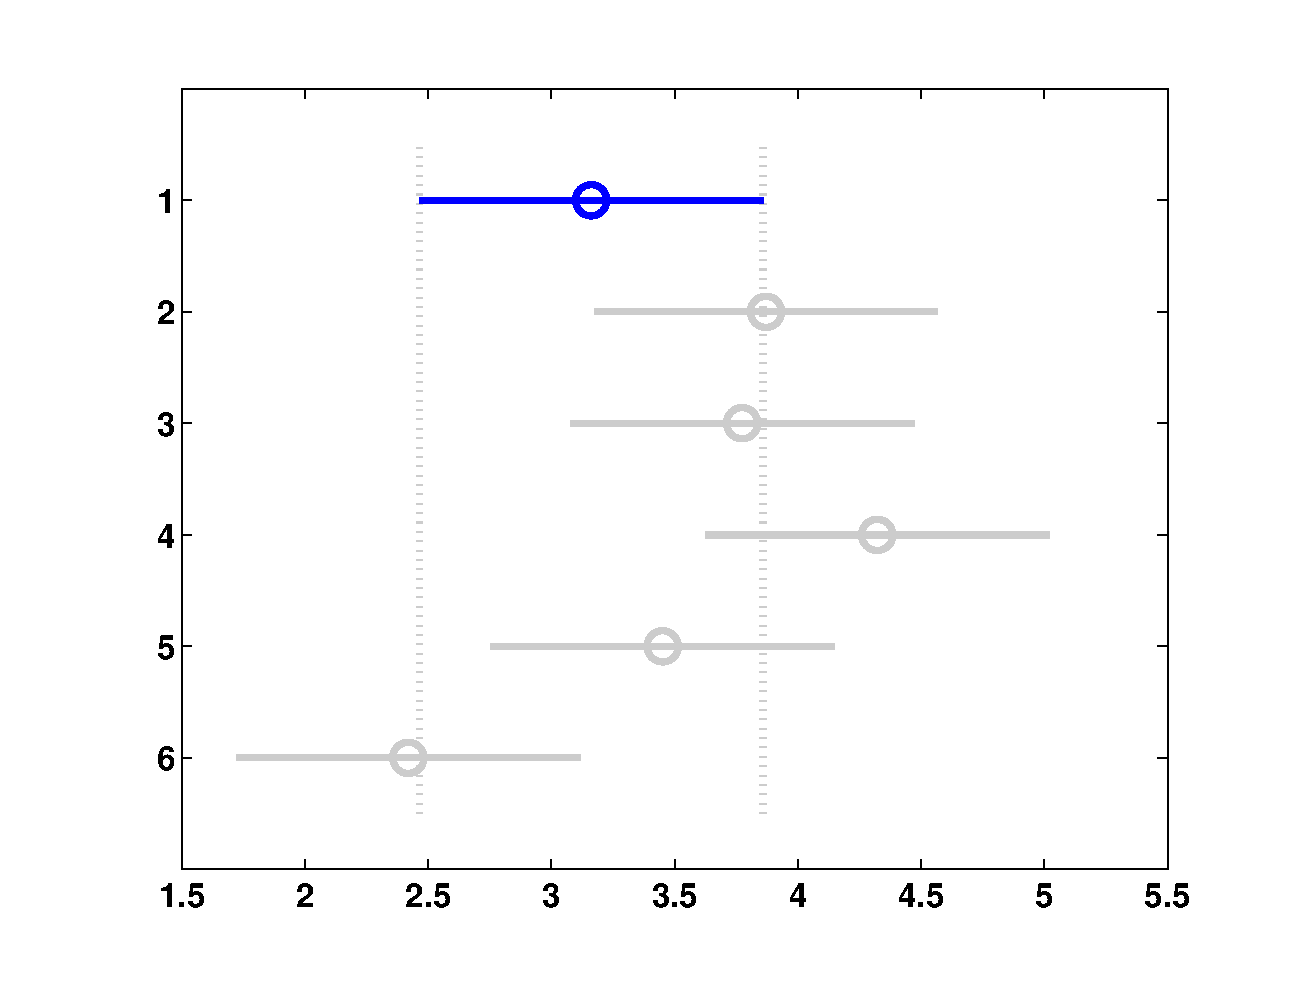
\includegraphics[width=\linewidth]{Figures/B-Bonferroni_HNMED_VS_ED6}
		\caption{SCE1} \label{fig:Bon_S1} 
	\end{subfigure}
	\caption[Resultados de las pruebas de Bonferroni-Dunn  obtenidos por las variantes HNMED vs ED/rand/1/bin en el Experimento B.]{Resultados de las pruebas de Bonferroni-Dunn  obtenidos por las variantes HNMED vs ED/rand/1/bin en el Experimento B. Se etiquetan en el eje vertical del 1 al 6 los algoritmos ED/rand/1/bin y HNMEDV1 a HNMEDV5   respectivamente.} \label{fig: Resultados de las pruebas de Bonferroni-Dunn para las variantes HNMED vs ED/rand/1/bin en el Experitmento B} 
	
\end{figure}
%


\subsubsection{Observaciones}
Los resultados obtenidos en la estadística descriptiva responden la primera pregunta de investigación planteada para el experimento B; ya que en efecto, las variantes propuestas son capaces de hallar valores iguales o mejores a los mínimos conocidos para todos los problemas de optimización a resolver. Las observaciones por cada problema son las siguientes:
\begin{enumerate}
	\item \textbf{MCE1}: Las variantes HNMED superan a la ED en las medidas de mejor y peor solución, promedio y desviación estándar. Ninguna logra superar el valor de la mediana de la ED. La variante HNMED con mejores resultados es V3.
	\item \textbf{MCE2}: Las variantes HNMED superan a la ED en todas las medidas. La variante con mejores resultados es V5.
	\item \textbf{MCE3}: Se iguala a la ED en la mejor y peor observación de la muestra. La ED supera a las variantes HNMED en los valores de mediana, promedio y desviación estándar.La variante con mejores resultados es la V3.
	\item \textbf{GCE1}: Las variantes supera a la ED en todas las medidas. HNMED-V5 presenta los mejores resultados.
	\item \textbf{GCE2}: Todas las variantes superan a la ED en su mejor y peor solución, excepto HNMED-V1. Sólo HNMED-V5 (variante con mejores resultados) supera la mediana de la ED la cual prevalece en las demás medidas (promedio y desviación estándar).
	\item \textbf{SCE1}: Todas las variantes superan a la ED en el mejor resultado, siendo HNMED-V5 la que logra superar a la ED en las medidas de promedio y mediana. 
\end{enumerate}
De forma general, las variantes propuestas presentan mejores valores en las medidas de tendencia central para la mayoría de los problemas y valores modestos de desviación estándar lo que indica cierta sensibilidad a la distribución inicial de la población. Se destacan además las medida de la mejor solución de la muestra en la cual las variantes siempre obtienen resultados iguales (para MCE2 y MCE3) o mejores (MCE1,GCE1,GCE2,SCE1) a la ED. Esto se debe a la capacidad de explotación de las instancias del método Nelder Mead.

En la Figura \ref{fig: Gráficas de convergencia para las variantes HNMED y ED/rand/1/bin} se observa que, para todos los problemas las curvas descritas por las variantes HNMED se encuentran por debajo a las de ED/rand/1/bin. Esto significa que todas las versiones pueden obtener resultados competitivos en un menor número de evaluaciones. También se puede observar que las curvas dadas por los algoritmos propuestos se encuentran ligeramente corridas a la izquierda, lo que indica que son capaces de encontrar individuos factibles en iteraciones tempranas. Este comportamiento se debe a la capacidad del simplex de muestrear el espacio de búsqueda con pocas evaluaciones. Es importante destacar que con los resultados obtenidos se demuestran dos aspectos principales robustez y eficiencia del enfoque propuesto. 

En la Tabla \ref{tab:Resultados Firedman obtenidos por variantes HNMED y DE/rand/1/bin  experimento B.} se observan los resultados obtenidos en la prueba de Friedman para cada problema:
\begin{enumerate}
	\item \textbf{MCE1}: El mejor promedio de jerarquía obtenido corresponde a la ED. Sin embargo, se acepta la hipótesis nula con un valor de $p=8.1173E-01$. Esto significa que a pesar de que la ED obtiene mejores resultados en este problema,  no se puede afirmar que son significativamente mejores y por lo tanto su desempeño es similar al obtenido por las variantes HNMED. La mejor jerarquía obtenida por las variantes HNMED corresponden a V5.
	\item \textbf{MCE2}: El algoritmo HNMED-V5  obtiene el mejor promedio de jerarquía. Además, todas las versiones HNMED obtienen una mejor jerarquía promedio con respecto a la ED. En este caso se rechaza la hipótesis nula con valor de $p=1.3277E-26$. En este problema se evidencia un desempeño significativamente mejor por parte de las 5 variantes propuestas en comparación con la ED.
	
	\item \textbf{MCE3}: La ED/rand/1/bin alcanza el mejor promedio de jerarquía. No obstante, se acepta la hipótesis nula con valor de $p=9.4985E-01$. Al igual que en la prueba para el problema MCE1 se concluye que existe un desempeño similar entre todos los algoritmos comparados.
	
	\item \textbf{GCE1}: De forma similar al problema MCE2 todas las variantes HNMED obtienen mejor jerarquía respecto a la ED, siendo la V5 el algoritmo ganador. La hipótesis nula se rechaza concluyendo que las versiones V5 se comportan significativamente mejor que la ED.
	
	\item \textbf{GCE2}: EL algoritmo ganador es HNMED-V5. Todas las versiones HNMED obtienen mejores jerarquías que la ED  a excepción de la V1. En este caso la hipótesis nula se acepta por lo tanto no se confirma que existen diferencias significativas entre el desempeño de las variantes ganadoras y la ED. 
	
	\item \textbf{SCE1}: En este caso se rechaza la hipótesis nula con valor de $p=1.7205E-03$, siendo HNMED-V5 el algoritmo con mejor promedio de jerarquía. Sin embargo, como se puede observar en la Subfigura F de la Figura \ref{fig: Resultados de las pruebas de Bonferroni-Dunn  para las variantes HNMED y ED/rand/1/bin}, las diferencias significativas se encuentran entre HNMED-V5 y las variantes V1 y V2.  
	 
\end{enumerate}
De forma general se observa un desempeño competitivo de las variantes propuestas, obteniéndose resultados significativamente mejores en 2 de los problemas y desempeño similar el resto con respecto a la ED/rand/1/bin. La variante HNMED-V5 consigue el mejor desempeño de forma general la cual obtiene mejor promedio de jerarquías en 4 de los 6 problemas de optimización. Los peores promedios de jerarquía se obtienen en los problemas MCE1,MCE3 y GCE2 los cuales presentan mayor dimensión, restricciones y complejidad de la función. A pesar de que las variantes propuestas ganan en rapidez de convergencia, heredan en cierta medida las deficiencias del método de búsqueda local cuyas operaciones están destinadas a la explotación. Por tanto, se presenta un decremento del desempeño para problemas de mayor dimensionalidad aunque este no es significativo.



%%%%%%%%%%%%%%%%%%%%%%%%%%%%%%%%%%%%%%%%%%%%%%%%%%%%%%%%%%%%%%%%%%%%%%%%%%%%%%%%%%%%%%%%%%%%%%





\subsection{Experimentos C : Comparación de Variantes HNMED vs ED con reducción del número de evaluaciones}
El experimento C se realiza para conocer de forma exacta el número de evaluaciones en las que, las variantes propuestas presentan un desempeño competitivo en comparación con la ED/rand/1/bin. Con la realización de estos experimentos se reúne información sobre las variables contempladas en la hipótesis de investigación (calidad de resultados y rapidez) que permitirá junto con los experimentos finales una aceptación o rechazo de la misma.  

\subsubsection{Definición de medidas}
Se obtiene para cada algoritmo una muestra de $n=31$ ejecuciones. Para cada problema las observaciones en la muestra corresponden al valor de la función objetivo del mejor individuo factible encontrado por el algoritmo $A_i$en la ejecución $j$ para $j= \{ 1,2,...,n\}$. Se aplicarán al conjunto de muestras las siguientes pruebas de estadística descriptiva e inferencial:
\begin{enumerate}

		\item \textbf{Estadística descriptiva}: Se obtiene la la mejor y peor solución, mediana, promedio y desviación estándar de las muestras
		\item \textbf{Gráfica de convergencia}: Se presenta la gráfica de convergencia correspondiente a la mediana de la muestra para cada algoritmo en comparación.
		\item \textbf{Prueba de Friedman}: con nivel significancia $\alpha=0.05$ para determinar si existen diferencias significativas entre el desempeño de al menos dos de los algoritmos comparados. 
		\item \textbf{Prueba Bonferroni-Dunn}: con nivel significancia $\alpha=0.05$ para determina entre cuáles de los algoritmos comparados existe una diferencia significativa de desempeño.

\end{enumerate}
\subsubsection{Planificación pre-experimental y configuración}
Para este experimento se mantuvo el número de evaluaciones realizadas por la ED según se describe en la literatura. El número de evaluaciones fue reducido para cada uno de los algoritmos en comparación en cada problema de optimización según se describe en la Tabla \ref{tab:Evaluaciones utilizadas por problema de optimización Experimentos C.}:

\begin{table}[]
	
	\caption{Evaluaciones utilizadas por problema de optimización Experimentos C.}
	\label{tab:Evaluaciones utilizadas por problema de optimización Experimentos C.}
	\centering
	\resizebox{\textwidth}{!}{%
		\begin{tabular}{ccccccc}
			\textbf{Problema} &  \textbf{ ED    } &\textbf{HNMED-V1}&\textbf{HNMED-V2}&\textbf{HNMED-V3}&\textbf{HNMED-V4}&\textbf{HNMED-V5  } \\
			\hline
			MCE1   &   750030 &500000 &400000&400000&400000&400000   \\
			MCE2   &   20000  &15000  &15000 &15000 &15000 &15000  \\
			MCE3   &   450018 &35000  &25000 &25000 &225000 &225000 \\
			GCE1   &   750030 &125000  &125000 &125000 &125000 &125000  \\
			GCE2   &   750030 &225000  &225000 &225000 &225000 &225000 \\
			SCE1   &   288000 &240000  &240000 &240000 &216000 &216000 \\
		\end{tabular}
	}
\end{table}
La configuración de parámetros utilizada por las variantes HNMED y la ED es la siguiente:
\begin{enumerate}
	\item Se establece la probabilidad de cruza $CR=\{0.8, 1\}$ para ED y HNMED para todos los problemas.
	\item Se establece el factor de escala $F=\{0.3, 0.9\}$ para ED y HNMED para todos los problemas.
	\item Para las variantes HNMED se establecieron los parámetros de reflexión $\alpha=2$, expansión $\gamma=1.05$ $\beta=0.5$ para todos los problemas.
	\item El tamaño de población utilizado se ajusta para cada algoritmo según la Tabla \ref{tab:Tamaños de población utilizados para cada problema en el Experimento C.}. Donde el valor $NS$ se refiere a la cantidad de símpleces utilizados los cuales determinan la población para cada problema $NP=NS(N+1)$ donde $N$  es la dimensión del problema.
\end{enumerate}

\begin{table}[]
	\centering
	\caption{Tamaños de población utilizados para cada problema en el Experimento C.}
	\label{tab:Tamaños de población utilizados para cada problema en el Experimento C.}
	\resizebox{\textwidth}{!}{%
		\begin{tabular}{cccccccccccc}
			& \textbf{ED/rand/1/bin } & \multicolumn{2}{l}{\textbf{HNMED-V1}}&\multicolumn{2}{l}{\textbf{HNMED-V2}} &\multicolumn{2}{l}{\textbf{HNMED-V3}} &\multicolumn{2}{l}{\textbf{HNMED-V4}} &\multicolumn{2}{l}{\textbf{HNMED-V5}}  \\
			\hline
			\textbf{Problema} & \textbf{NP}            & \textbf{NS}          & \textbf{NP}   & \textbf{NS}          & \textbf{NP} & \textbf{NS}          & \textbf{NP}& \textbf{NS}          & \textbf{NP}& \textbf{NS}          & \textbf{NP}           \\
			\hline
			MCE1     & 138           & 9           & 144 &8&128&8&128&7&112&7&112        \\
			MCE2     & 50            & 3           & 21  &4&28&4&28&3&21&3&21        \\
			MCE3     & 138           & 7           & 140 &7&140&7&140&7&140&7&140        \\
			GCE1     & 138           & 9           & 135 &9&135&9&135&9&135&9&135        \\
			GCE2     & 138           & 9           & 135 &9&135&9&135&9&135&9&135      \\
			SCE1     & 50            & 7           & 35  &7&35&7&35&7&35&7&35       
		\end{tabular}
	}
\end{table}


\subsubsection{Presentación de resultados}
La Tabla \ref{tab:Resultados estadísticos obtenidos por variantes HNMED y DE/rand/1/bin  en experimento C.} muestra los resultados estadísticos obtenidos para cada problema indicando la reducción de evaluaciones en porciento. En la Figura \ref{fig: Gráficas de convergencia para las variantes HNMED y ED/rand/1/bin para el Experimento C} se muestra las gráficas de convergencias. La Tabla \ref{tab:Resultados de la prueba de Friedman en las variantes HNMED y DE/rand/1/bin en el experimento C para los seis problemas de diseño mecatrónico.} presenta los resultados de la prueba de Friedman y en la Figura \ref{fig: Resultados de las pruebas de Bonferroni-Dunn para las variantes HNMED vs ED/rand/1/bin en el experimento C.} contiene las pruebas post hoc de Bonferroni-Dunn para los 6 problemas de optimización.
%%%%%%%%%%%%%%%%%%%%%%%%%%%%%%%%%%%%%%%%%%%%%%%%%%%%%%%%%%%%%%%%%%%%%%%%%%%%%%%%%%%%%%%%%%%%%%%%%%%


\begin{table}
	
	\caption[Resultados estadísticos obtenidos por las variantes HNMED y DE/rand/1/bin en el Experimento C para los seis problemas de optimización.]{Resultados estadísticos obtenidos por las variantes HNMED y DE/rand/1/bin en el Experimento C para los seis problemas de optimización. Se marcan en negritas los mejores valores de cada medida.}\label{tab:Resultados estadísticos obtenidos por variantes HNMED y DE/rand/1/bin  en experimento C.}
	
	\centering
	\resizebox{\textwidth}{!}{%
		\begin{tabular}{clcccccc} 
			\hline
			Problema              & Estadística   & HNMED-V1    & HNMED-V2    &HNMED-V3      &HNMED-V4      & HNMED-V5     & ED/rand/1/bin  \\ 
			\hline
			\multirow{6}{*}{MCE1} & Mejor       & 5.80602E-28&	\textbf{1.26218E-29}	   &5.04871E-29  &6.31089E-29	&4.9224E-29  &1.7670E-28 \\
			& Peor        & 3.1713E-02    &2.7676E-02    & 2.9936E-02  & \textbf{2.7424E-02}   & 2.7432E-02   & 2.7649E-02 \\
			& Mediana     & 3.4667E-04    & 3.9921E-04   & 4.5762E-04  & 3.9547E-04   & 3.4607E-04   & \textbf{4.2746E-06}   \\
			& Promedio    & \textbf{3.1573E-03}    & 4.7172E-03   & 7.1235E-03   & 4.5629E-03  & 6.9630E-03   & 2.9850E-01  \\
			& Desv. Est.  & 8.7501E-03    &1.0145E-02    & \textbf{1.1201E-03}   & 4.9555E-03  & 1.1579E-03   & 8.1906E-03  \\
			& Evaluaciones & 500000(-33\%)&400000 (-46.66\%) &400000 (-46.66\%)   & 400000 (-46.66\%) & 400000 (-46.66\%)   & 750030 \\
			
			\hline
			\multirow{6}{*}{MCE2} & Mejor       & 2.6280E-03   &2.6280E-03   &2.6280E-03    & 2.6280E-03    & 2.6280E-03   &2.6280E-03 \\
			& Peor        &2.8317E-03   & \textbf{2.6280E-03 }  & \textbf{2.6280E-03  }   & \textbf{2.6280E-03}  & \textbf{2.6280E-03  } & 2.6426E-03\\
			& Mediana     & 2.6280E-03   &2.6280E-03   & 2.6280E-03    & 2.6280E-03   & 2.6280E-03   & 2.6280E-03   \\
			& Promedio    & 2.6349E-03    &\textbf{2.6280E-03 }  & \textbf{2.6280E-03  }  &\textbf{ 2.6280E-03 } & \textbf{2.6280E-03 }  & 2.6288E-03 \\
			& Desv. Est.  & 4.6798e-03    & \textbf{8.3771E-10 }&2.2862E-09    &  6.8497E-08 & 2.8769E-09   & 2.7205E-06 \\
			& Evaluaciones&\textbf{15000}(-33.3\%) &\textbf{15000}(-33.3\%)  &\textbf{15000}(-33.3\%) & \textbf{15000}(-33.3\%)  & \textbf{15000}(-33.3\%)  &20000  \\     
			
			\hline
			\multirow{6}{*}{MCE3} & Mejor       & 2.7496E-01    & 2.7527E-01   & 2.7496E-01   &2.7496E-01   & 2.7496E-01    & 2.7496E-01  \\
			& Peor        & 1.3508E+01    & 1.3508E+01   & 1.3508E+01   & 1.3508E+01   & 1.3508E+01   & 1.3508E+01 \\
			& Mediana     & 7.3675E-01   & 7.5977E+01   & 1.6433E+00  & 5.4040E-01   & 8.8976E-01   & \textbf{2.7563E-01}   \\
			& Promedio    & 5.1387E+00   & 5.6636E+00    & 5.79209E+00  & 4.6850E+00   & 5.6552E+00   & \textbf{1.2313E+00} \\
			& Desv. Est.  & 6.3164E+00   & 6.6190E+00    & 6.2649E+00   & 6.1952E+00   & 6.3652E+00   & \textbf{8.1906E-03}  \\
			& Evaluaciones&350000(-22.2\%) &250000(-44.4\%) &250000(-44.4\%)   & 225000(-50.0\%)   & \textbf{225000}(-50.0\%)  & 450018 \\
			
			
			\hline
			\multirow{6}{*}{GCE1} & Mejor       & 6.3108E-29    &\textbf{ 0 }          &\textbf{ 0   }         &\textbf{ 0}            &\textbf{ 0 }           &6.7147E-27 \\
			& Peor        &1.7951E-26    & 1.9090E-27   & 4.7773E-27   & 2.0699E-27   & \textbf{9.0876E-28}  & 5.9926E-20 \\
			& Mediana     &2.47387E-27  & 5.0487E-29   & 5.04871-29   & 5.6797E-29   & \textbf{1.2621E-29}   & 3.9485E-23  \\
			& Promedio    &3.80302E-27   &2.3248E-28    & 4.8268E-28  & 2.4801E-28   &\textbf{ 6.2396E-29 } & 3.4957E-21  \\
			& Desv. Est.  & 4.36121E-27    &4.8191E-28   &	1.1600E-27  & 4.4014E-28   &\textbf{ 1.6612E-28}   & 1.2077E-20  \\
			& Evaluaciones&\textbf{125000}(-83.3\%) &\textbf{125000}(-83.3\%) &\textbf{125000}(-83.3\%)    & \textbf{125000}(-83.3\%)    & \textbf{125000}(-83.3\%)  & 750030\\
			
			
			\hline
			\multirow{6}{*}{GCE2} & Mejor       &\textbf{1.1385E-01}&1.4713E-02&\textbf{	1.1385E-01	}&\textbf{1.1385E-01}&	\textbf{1.1385E-01 }        &1.1388E-01 \\
			& Peor        &1.89116E-01&	2.3328E-01&	1.7400E-01&	\textbf{1.5932E-01}&	1.6559E-01    &1.6075E-01 \\
			& Mediana     &1.5513E-01&	1.5417E-01&	1.1746E-01&	1.5202E-01&	1.5294E-01 & \textbf{1.1447E-01}  \\
			& Promedio    & 1.4773E-01&	1.4407E-01&	1.3132E-01&	1.3611E-01&	1.3934E-01 &\textbf{ 1.2080E-01 } \\
			& Desv. Est.  &2.1528E-02&	2.6887E-02	&2.06472E-02	&2.0660E-02	&2.0410E-02& \textbf{1.4713E-02 }\\
			& Evaluaciones &\textbf{250000}(-44.4\%) &\textbf{250000}(-44.4\%) &\textbf{250000}(-44.4\%)  & \textbf{250000}(-44.4\%)  &\textbf{225000}(-50.0\%)  &  450018 \\
			
			
			
			
			
			\hline
			\multirow{6}{*}{SCE1} & Mejor       & -5.7452E+05    & -5.7725E+05    & \textbf{-5.8217E+05}   &-5.7364E+05   & -5.3652E+05   &-5.3206E+05 \\
			& Peor        &-4.9379E+05     & -4.9669E+o5   & -5.2250E+05   & -5.2442E+05  & -5.3080E+05  & \textbf{-5.3204E+05} \\
			& Mediana     &-5.3667E+05    &-5.3083E+05   & -5.3188E+05   & -5.3175E+05   & \textbf{-5.3217E+05}  & -5.3205E+05   \\
			& Promedio    &-5.3690E+05   &-5.33062E+05   & -5.4196E+05   & -5.3292E+05   & \textbf{-5.3230E+05 }  & -5.3205E+05 \\
			& Desv. Est.  &1.9677E+04  & 1.7853E+04    & 1.9516E+04   & 7.9197E+03   & 1.0945E+03  & \textbf{3.3010E+00 } \\
			& Evaluaciones&240000 (-8.3 \%) & 240000 (-16.6 \%)  & 240000 (-16.6 \%)   & \textbf{216000} (-25.0 \%) & \textbf{216000} (-25.0 \%)&288000
			
			
			
			
			
		\end{tabular}
	}
\end{table}
\begin{figure}
	\centering
	\begin{subfigure}[b]{0.49\linewidth}
		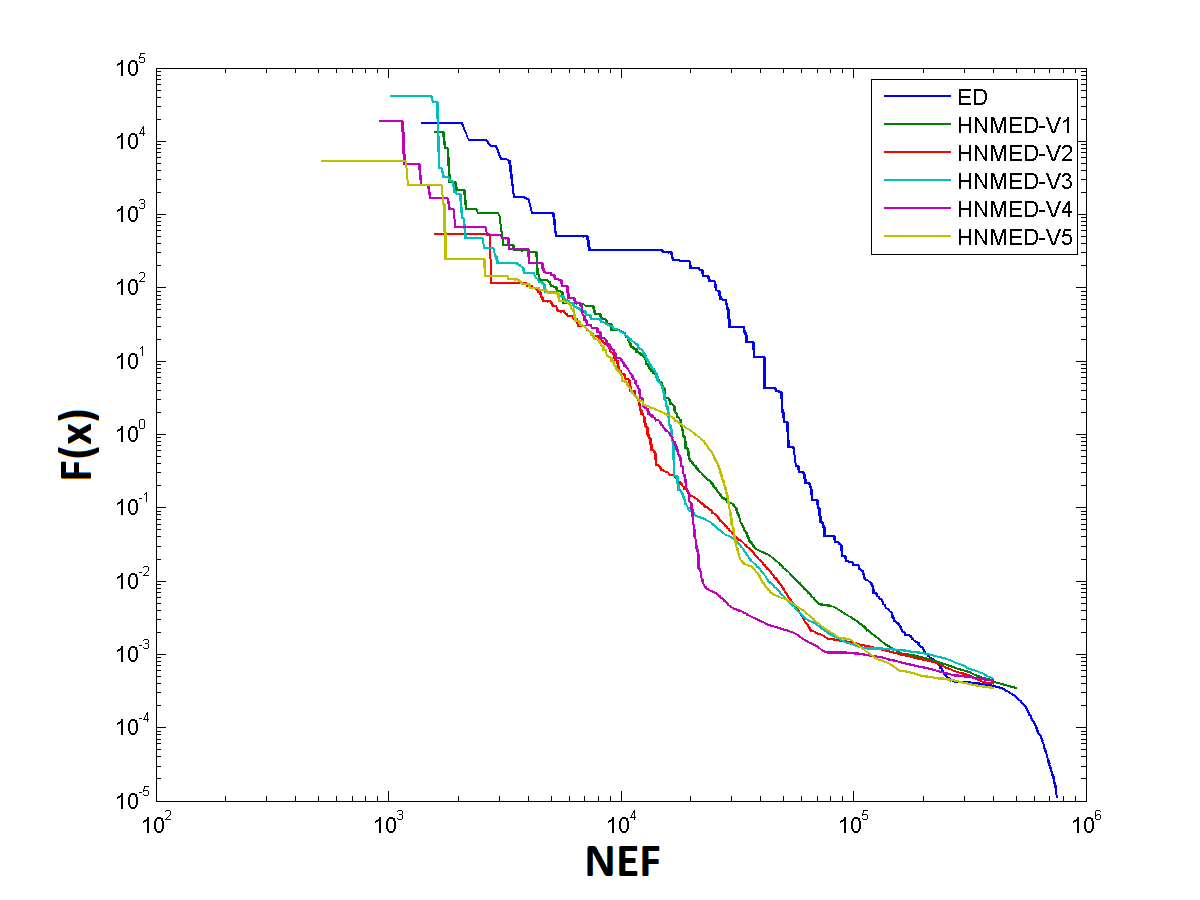
\includegraphics[width=\linewidth]{Figures/C-Grafica_Convergencia_Problema_1}
		\caption{MCE1} \label{fig:M1} 
	\end{subfigure}
	\begin{subfigure}[b]{0.49\linewidth}
		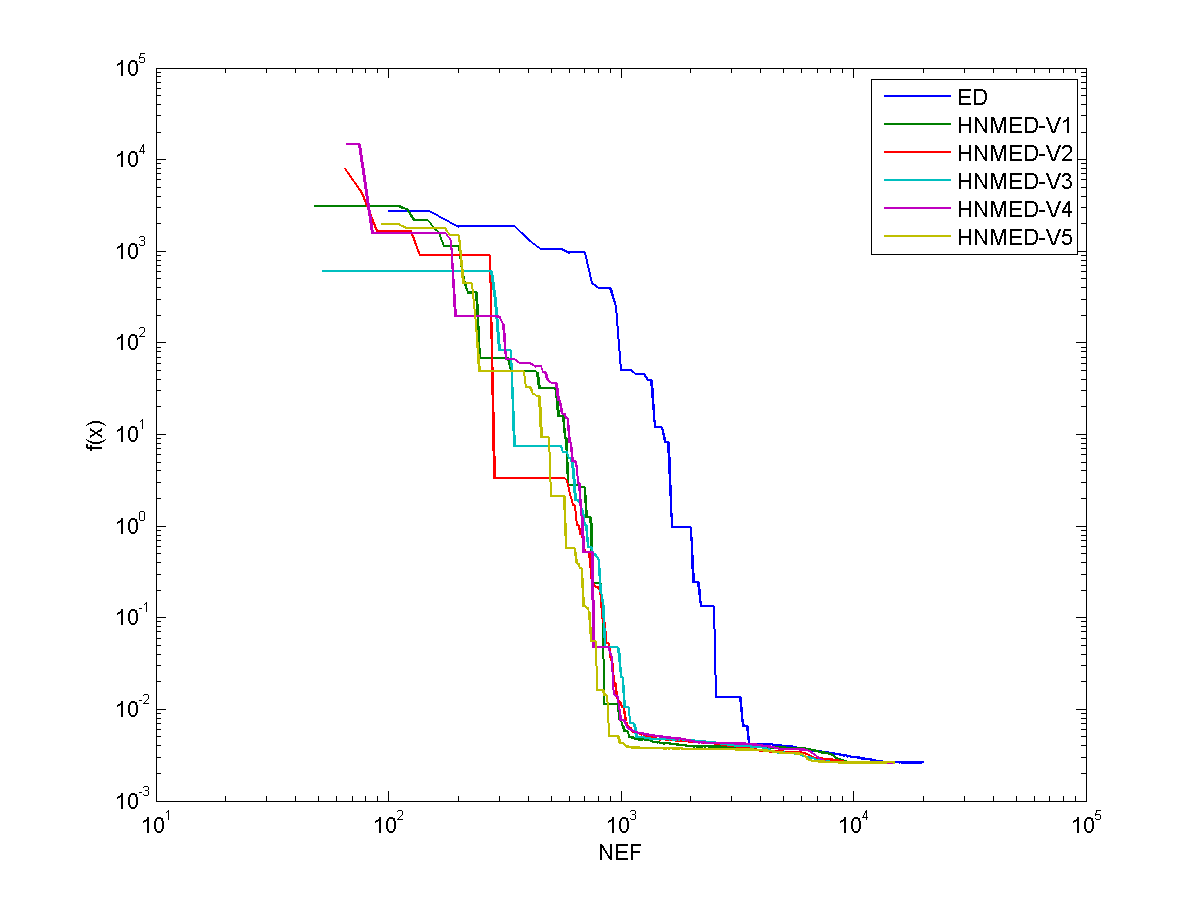
\includegraphics[width=\textwidth]{Figures/C-Grafica_Convergencia_Problema_2}
		\caption{MCE2} \label{fig:M2} 
	\end{subfigure}
	\begin{subfigure}[b]{0.49\linewidth}
		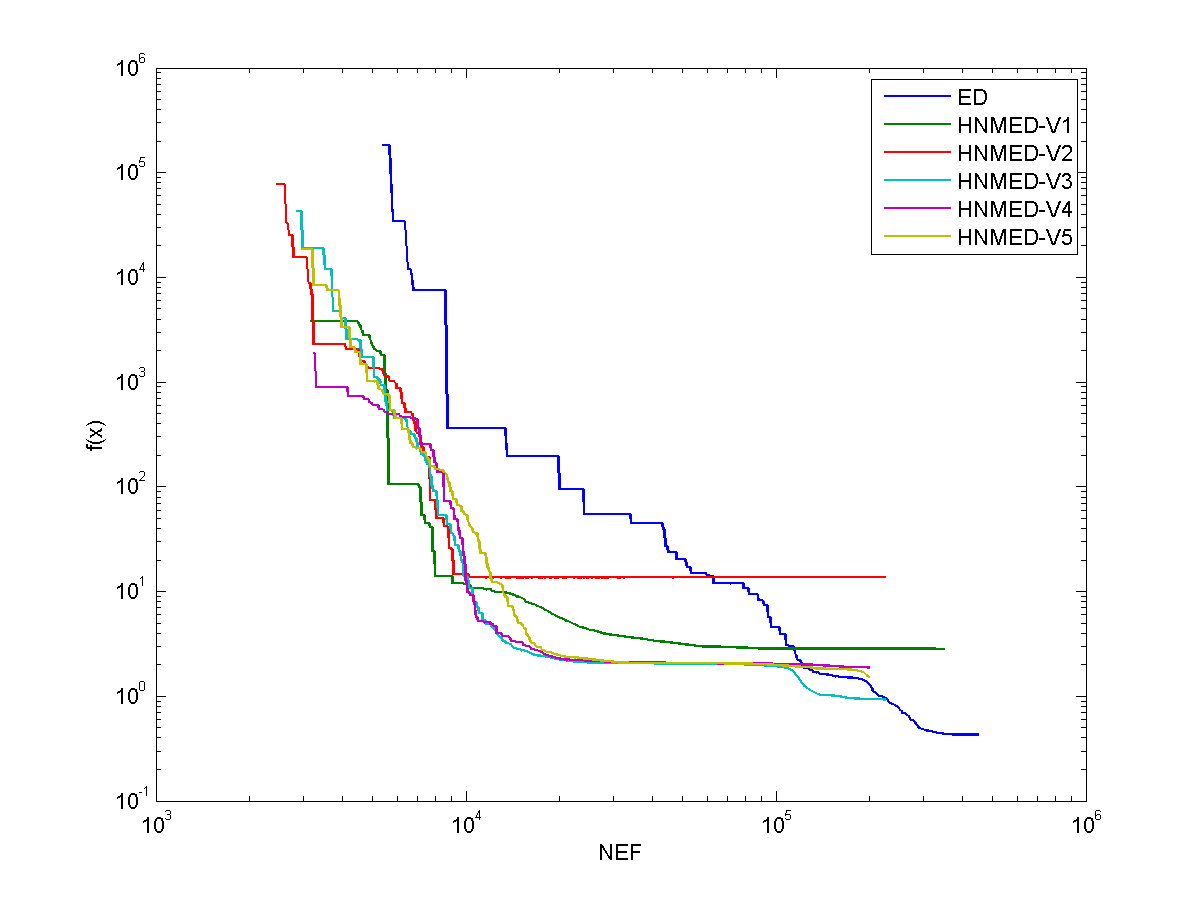
\includegraphics[width=\linewidth]{Figures/C-Grafica_Convergencia_Problema_3}
		\caption{MCE3} \label{fig:M3} 
	\end{subfigure}
	\begin{subfigure}[b]{0.49\linewidth}
		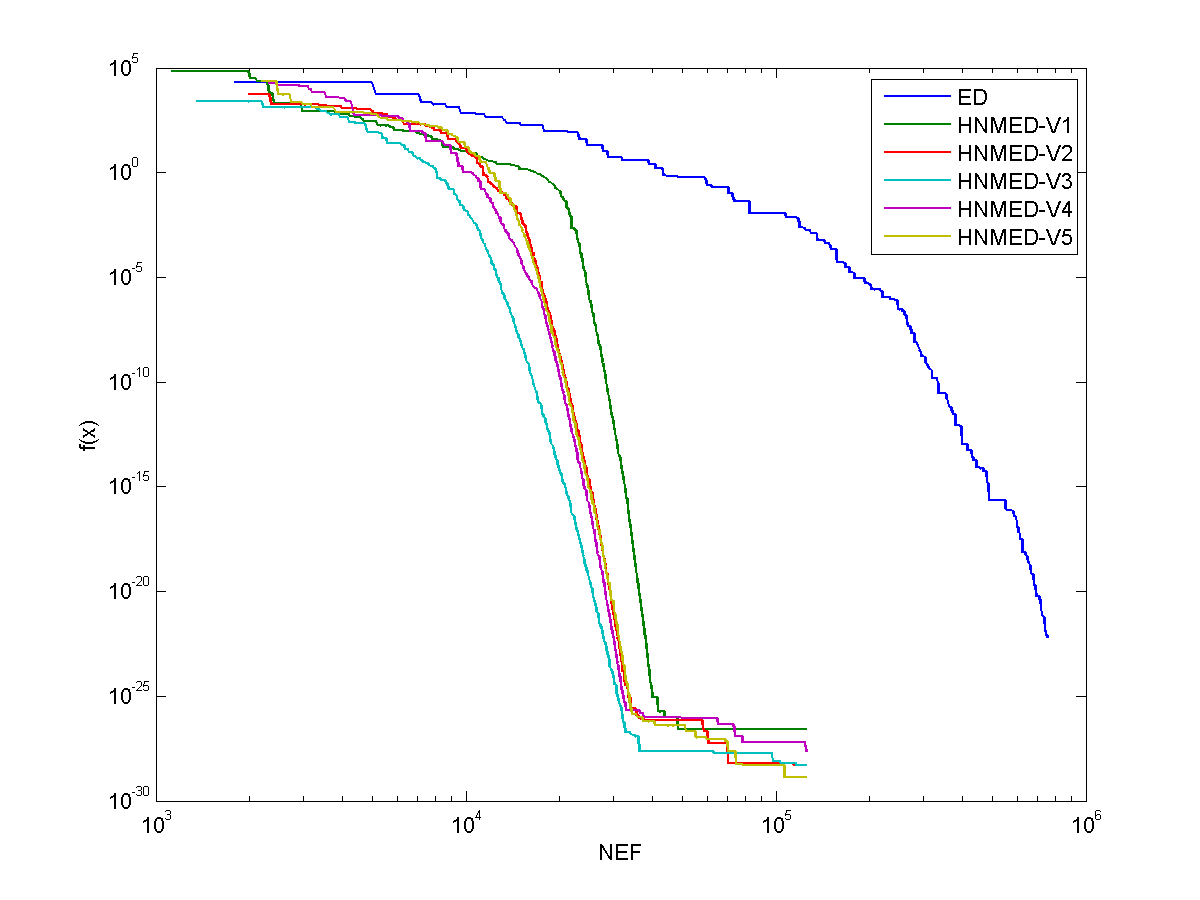
\includegraphics[width=\linewidth]{Figures/C-Grafica_Convergencia_Problema_4}
		\caption{GCE1} \label{fig:G1} 
	\end{subfigure}
	\begin{subfigure}[b]{0.49\linewidth}
		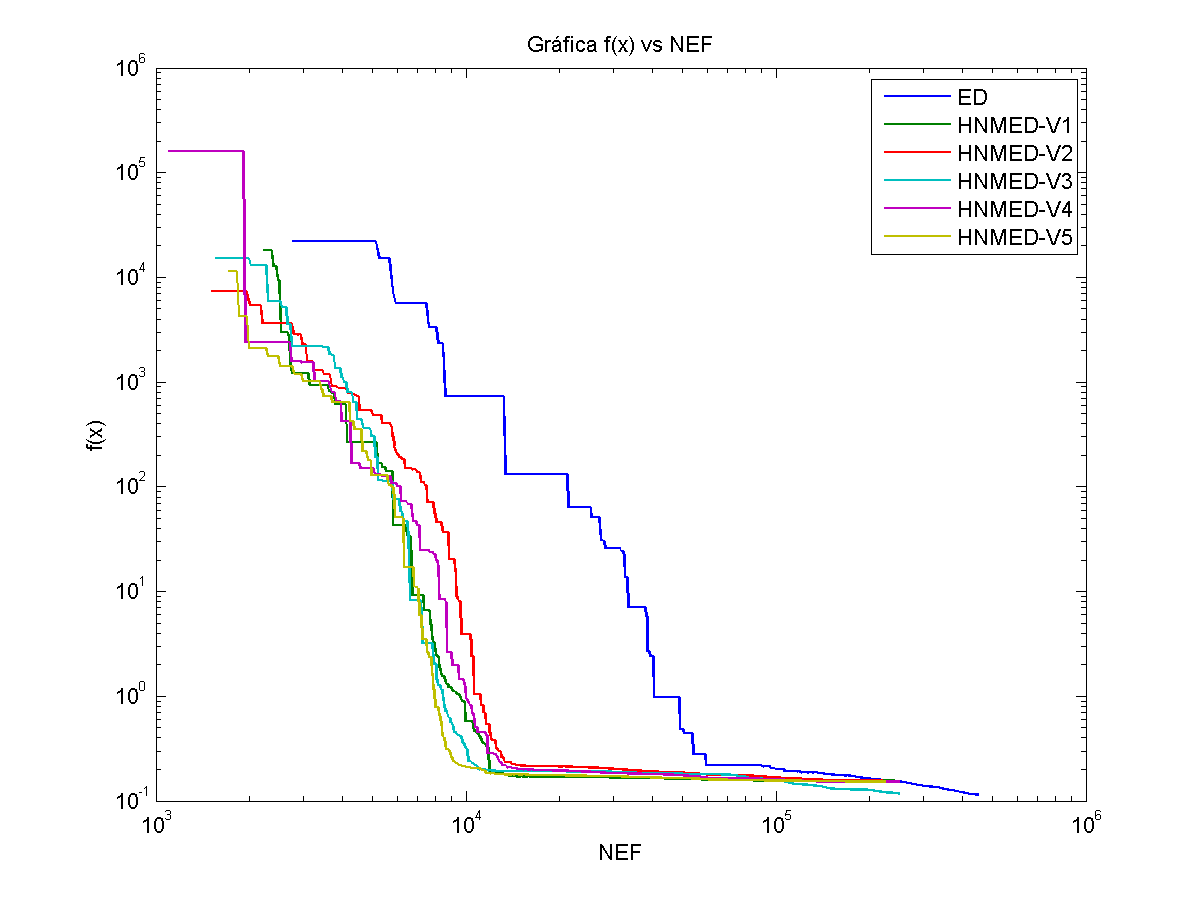
\includegraphics[width=\linewidth]{Figures/C-Grafica_Convergencia_Problema_5}
		\caption{GCE2} \label{fig:G2} 
	\end{subfigure}
	\begin{subfigure}[b]{0.49\linewidth}
		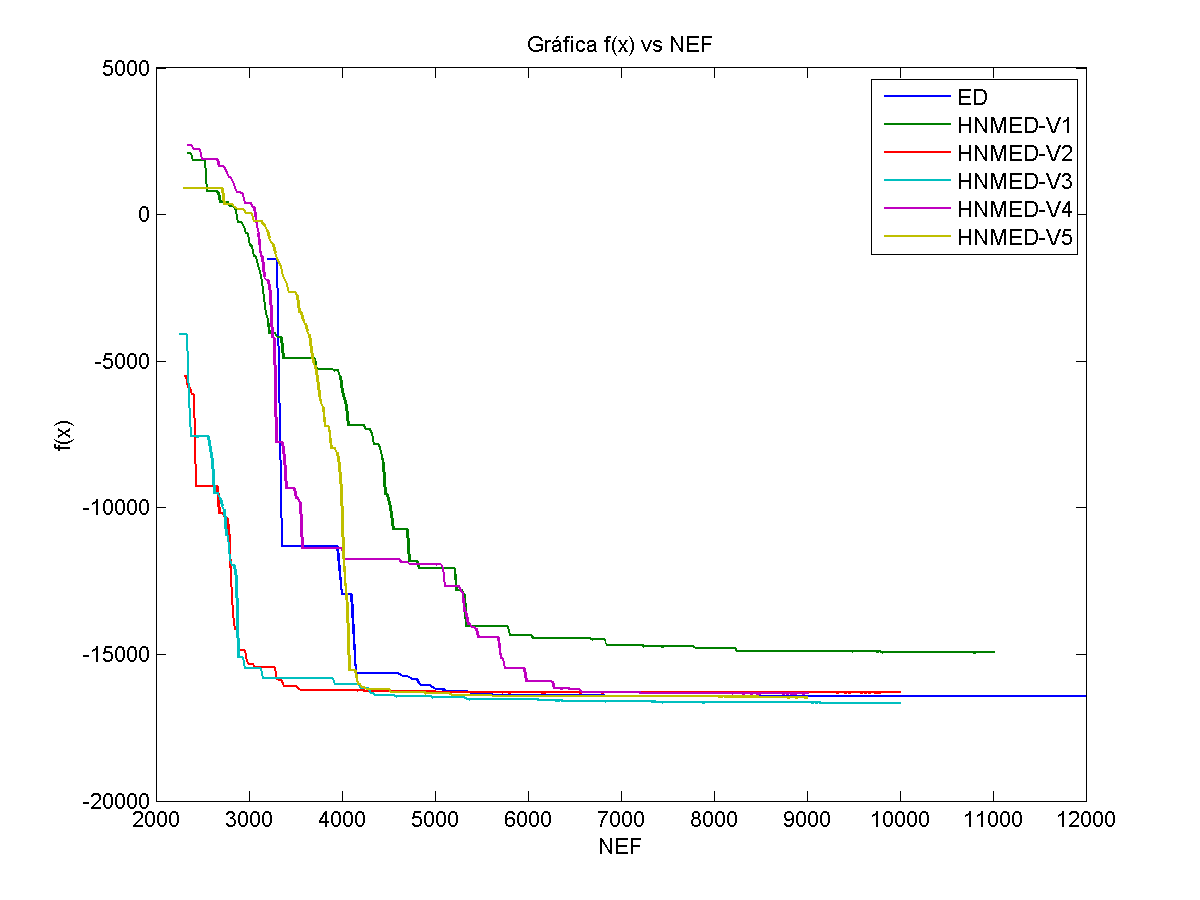
\includegraphics[width=\linewidth]{Figures/C-Grafica_Convergencia_Problema_6}
		\caption{SCE2} \label{fig:S1} 
	\end{subfigure}
	\caption[Gráficas de convergencia obtenidas por las variantes HNMED y ED/rand/1/bin en el Experimento C.]{Gráficas de convergencia obtenidas por las variantes HNMED y ED/rand/1/bin en el Experimento C. El eje horizontal presenta el número de evaluaciones de la función objetivo (NEF) y el eje vertical el valor de  $f(x)$.} \label{fig: Gráficas de convergencia para las variantes HNMED y ED/rand/1/bin para el Experimento C} 
	
\end{figure}
\begin{table}
	\centering
	\caption[Resultados de la prueba de Friedman obtenidos por las variantes HNMED y DE/rand/1/bin en el experimento C para los seis problemas de diseño mecatrónico.]{Resultados de la prueba de Friedman obtenidos por las variantes HNMED y DE/rand/1/bin en el experimento C para los seis problemas de diseño mecatrónico. Se resaltan en negritas los promedios de jerarquías ganadores}
	\label{tab:Resultados de la prueba de Friedman en las variantes HNMED y DE/rand/1/bin en el experimento C para los seis problemas de diseño mecatrónico.}
	\resizebox{\textwidth}{!}{%{0.3132\textheight}{%
		\begin{tabular}{lccccc}
			\hline
			Problema              & Algoritmo     & Jerarquía promedio &Valor de $p$        & $H_0$                           & $H_1$             \\
			\hline  
			\multirow{6}{*}{MCE1} & HNMED-V1      &3.6451E+00          &\multirow{6}{*}{1.1011E-02}  & \multirow{6}{*}{Rechazada}& \multirow{6}{*}{Aceptada} \\
			& HNMED-V2      & 3.3870E+00        &                    &                          &                            \\
			& HNMED-V3      &  4.0000E+00       &                    &                          &                            \\
			& HNMED-V4      &  3.9677E+00        &                    &                          &                            \\
			& HNMED-V5      &  3.5806E+00        &                    &                          &                            \\
			& ED/rand/1/bin &\textbf{2.4193E+00} &                    &                          &                            \\
			
			\hline  
			\multirow{6}{*}{MCE2} & HNMED-V1      & 3.7096E+00         & \multirow{6}{*}{2.1026E-12} & \multirow{6}{*}{Rechazada}& \multirow{6}{*}{Aceptada} \\
			& HNMED-V2      &3.0322E+00&                    &                          &                            \\
			& HNMED-V3      & 2.74193E+00         &                    &                          &                            \\
			& HNMED-V4      & 2.9032E+00         &                    &                          &                            \\
			& HNMED-V5      &\textbf{2.7741E+00 }&                    &                          &                            \\
			& ED/rand/1/bin &   5.8387E+00       &                    &                          &                            \\
			\hline
			
			\multirow{6}{*}{MCE3} & HNMED-V1      &  3.580645        & \multirow{6}{*}{4.4788E-03}  & \multirow{6}{*}{Rechazada}& \multirow{6}{*}{Aceptada} \\
			& HNMED-V2      & 4.0000E+00        &                    &                          &                            \\
			& HNMED-V3      & 3.9193E+00         &                    &                          &                            \\
			& HNMED-V4      & 3.5806E+00         &                    &                          &                            \\
			& HNMED-V5      &  3.6290E+00         &                    &                          &                            \\
			& ED/rand/1/bin & \textbf{2.2903E+00}    &                    &                          &                            \\
			
			
			
			\hline  
			\multirow{6}{*}{GCE1} & HNMED-V1      &   4.6451E+00       & \multirow{6}{*}{1.3274E-20}  & \multirow{6}{*}{Rechazada}& \multirow{6}{*}{Aceptada} \\
			& HNMED-V2      &   2.500E+00       &                    &                          &                            \\
			& HNMED-V3      &   2.6290E+00       &                    &                          &                            \\
			& HNMED-V4      &   3.4354E+00       &                    &                          &                            \\
			& HNMED-V5      &\textbf{1.8870E+00} &                    &                          &                            \\
			& ED/rand/1/bin &   5.9032E+00       &                    &                          &                            \\
			\hline  
			
			\multirow{6}{*}{GCE2} & HNMED-V1      &  4.5483E+00        & \multirow{6}{*}{3.9377E-03}  & \multirow{6}{*}{Rechazada}& \multirow{6}{*}{Aceptada} \\
			& HNMED-V2      &  3.8709E+00        &                    &                          &                            \\
			& HNMED-V3      & \textbf{ 3.0322E+00}                    &                          &                          &  \\
			& HNMED-V4      &  3.2580E+00         &                    &                          &                            \\
			& HNMED-V5      & 3.7741E+00          &                    &                          &                            \\
			& ED/rand/1/bin & 2.5161E+00&        &                     &                            \\
			\hline 
			
			\multirow{6}{*}{SCE1} & HNMED-V1      & 3.1935E+00                   & \multirow{6}{*}{ 3.2643E-02 }  & \multirow{6}{*}{Rechazada}& \multirow{6}{*}{Aceptada} \\
			& HNMED-V2      & 4.3225E+00                   &                    &                          &                            \\
			& HNMED-V3      & 3.3870E+00                   &                    &                          &                            \\
			& HNMED-V4      & 3.9032E+00                   &                    &                          &                            \\
			& HNMED-V5      & \textbf{2.8709E+00 }         &                    &                          &                            \\
			& ED/rand/1/bin &3.3225E+00 &                  &                    &                            \\
			
		\end{tabular}
	}
\end{table}



% Pruebas de Bunferroni

\begin{figure}
	\centering
	\begin{subfigure}[b]{0.49\linewidth}
		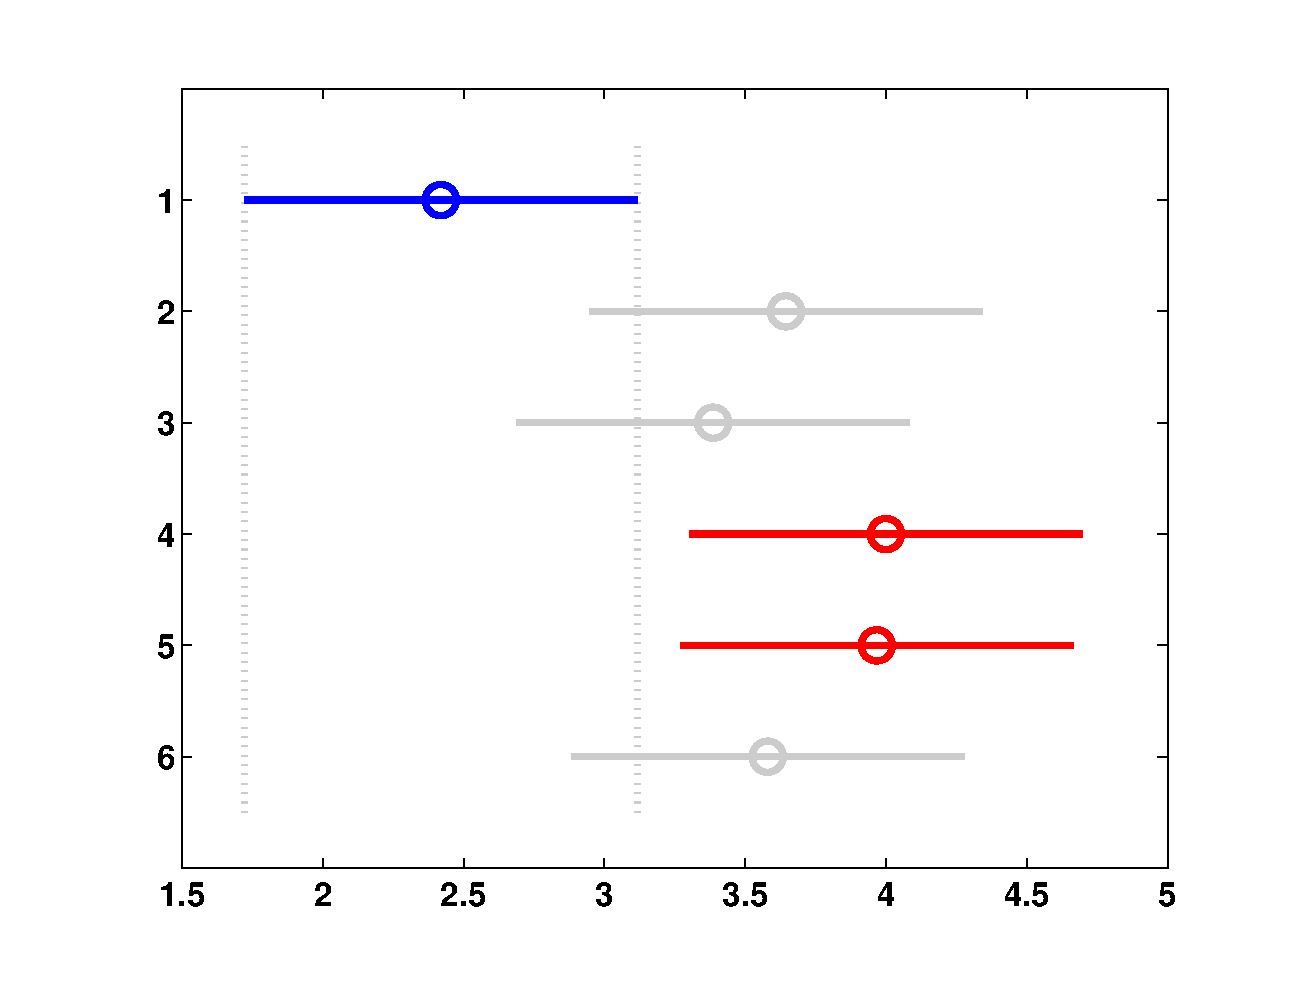
\includegraphics[width=\linewidth]{Figures/C-Bonferroni_HNMED_VS_ED1}
		\caption{MCE1} \label{fig:Bon_M1} 
	\end{subfigure}
	\begin{subfigure}[b]{0.49\linewidth}
		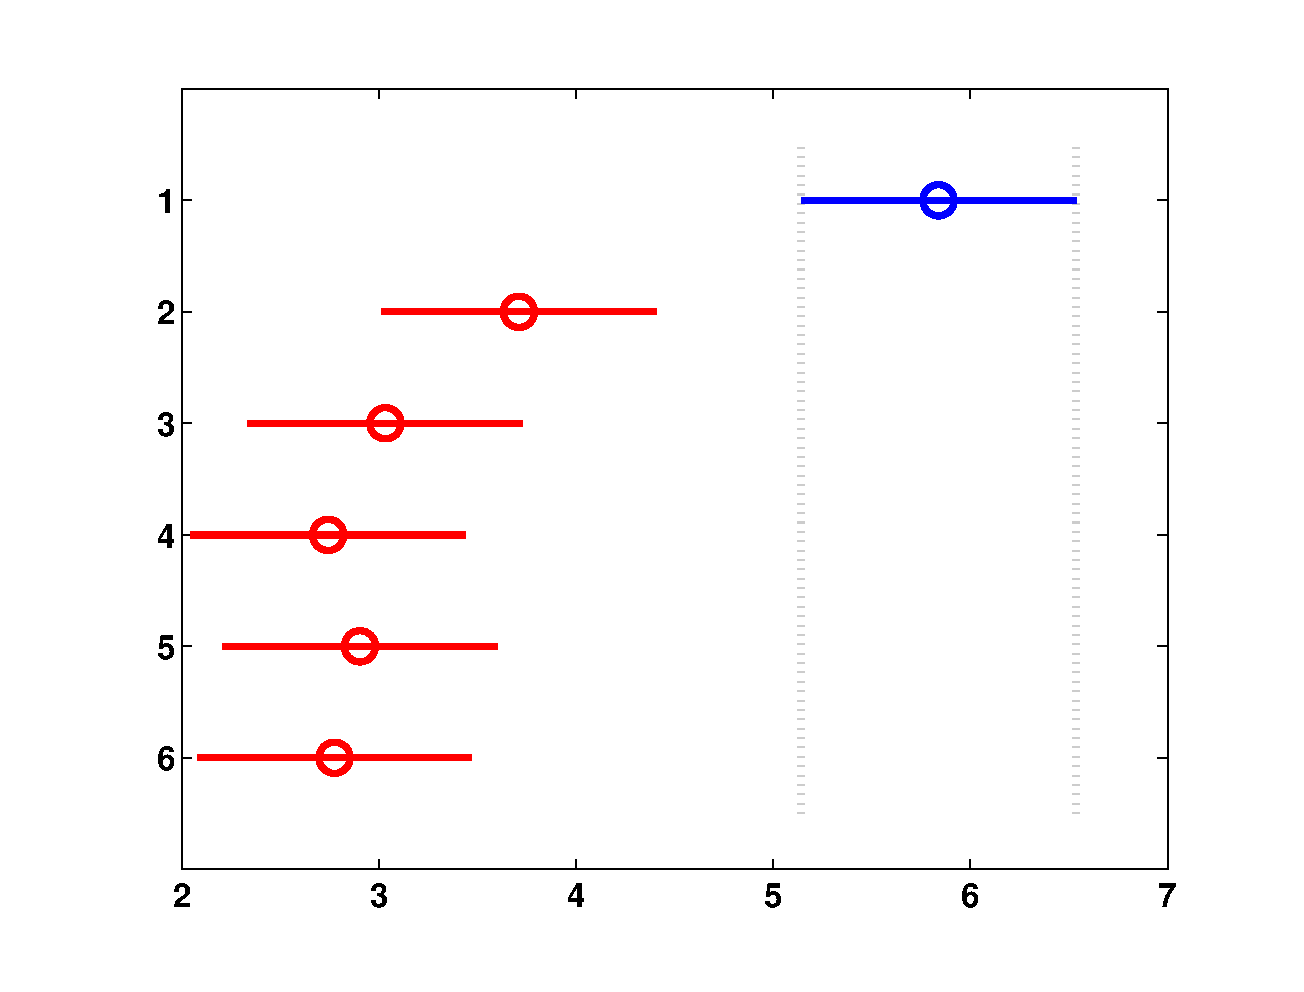
\includegraphics[width=\textwidth]{Figures/C-Bonferroni_HNMED_VS_ED2}
		\caption{MCE2} \label{fig:Bon_M2} 
	\end{subfigure}
	\begin{subfigure}[b]{0.49\linewidth}
		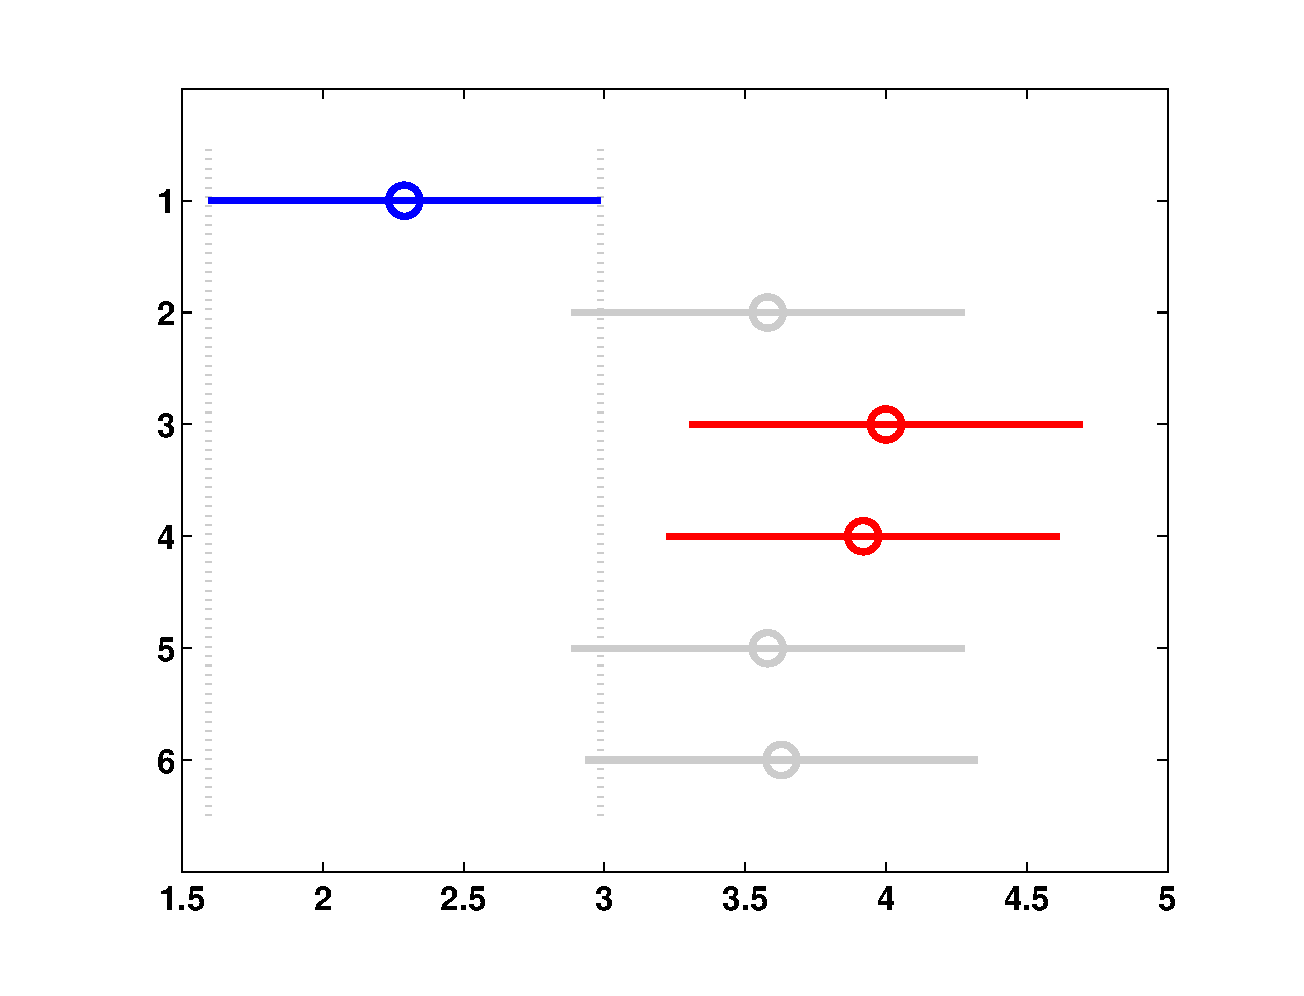
\includegraphics[width=\linewidth]{Figures/C-Bonferroni_HNMED_VS_ED3}
		\caption{MCE3} \label{fig:Bon_M3} 
	\end{subfigure}
	\begin{subfigure}[b]{0.49\linewidth}
		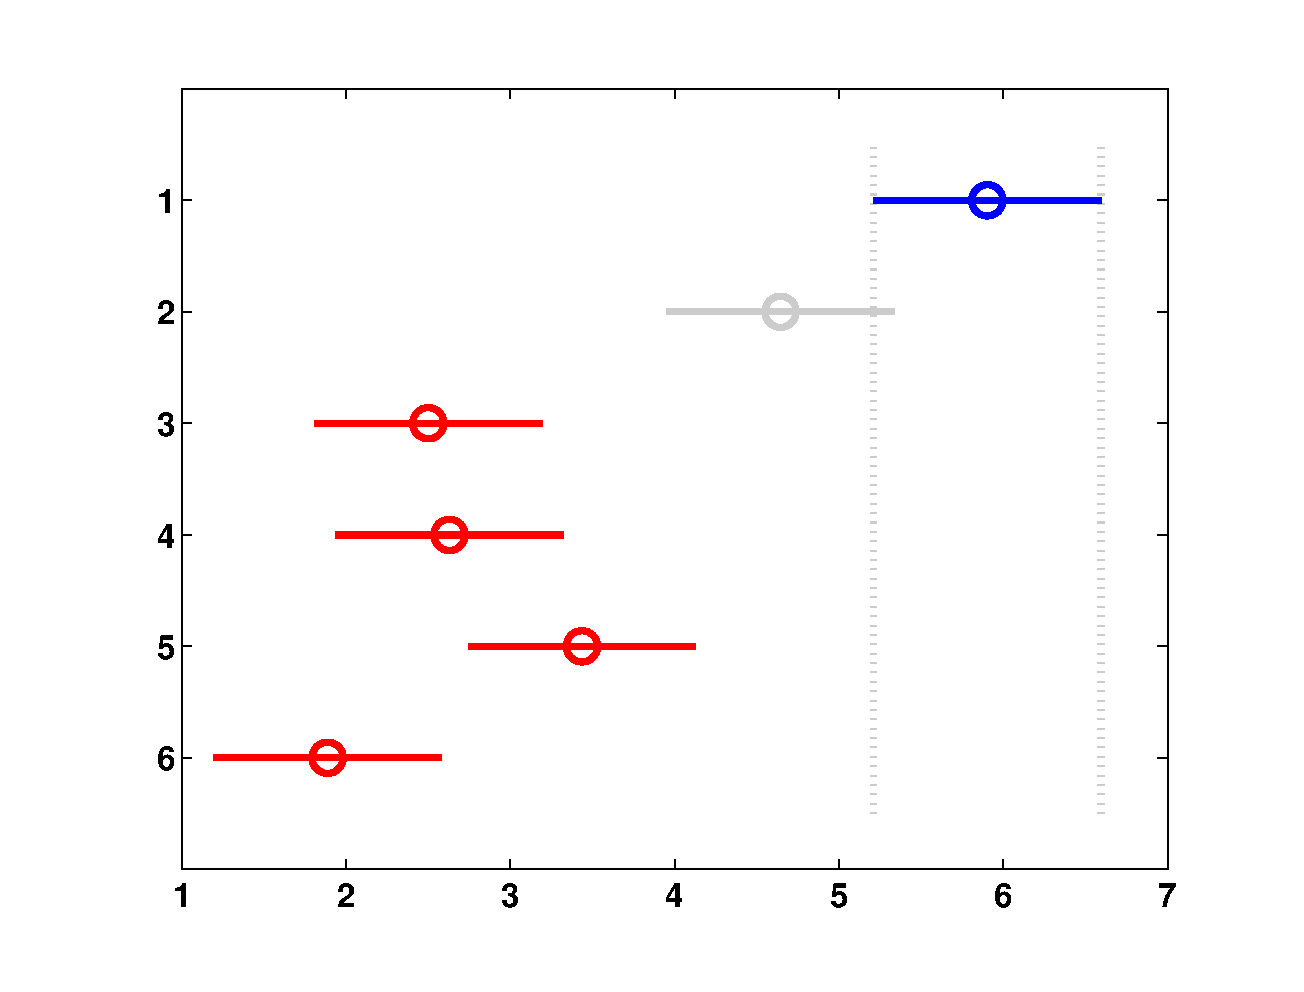
\includegraphics[width=\linewidth]{Figures/C-Bonferroni_HNMED_VS_ED4}
		\caption{GCE1} \label{fig:Bon_G1} 
	\end{subfigure}
	\begin{subfigure}[b]{0.49\linewidth}
		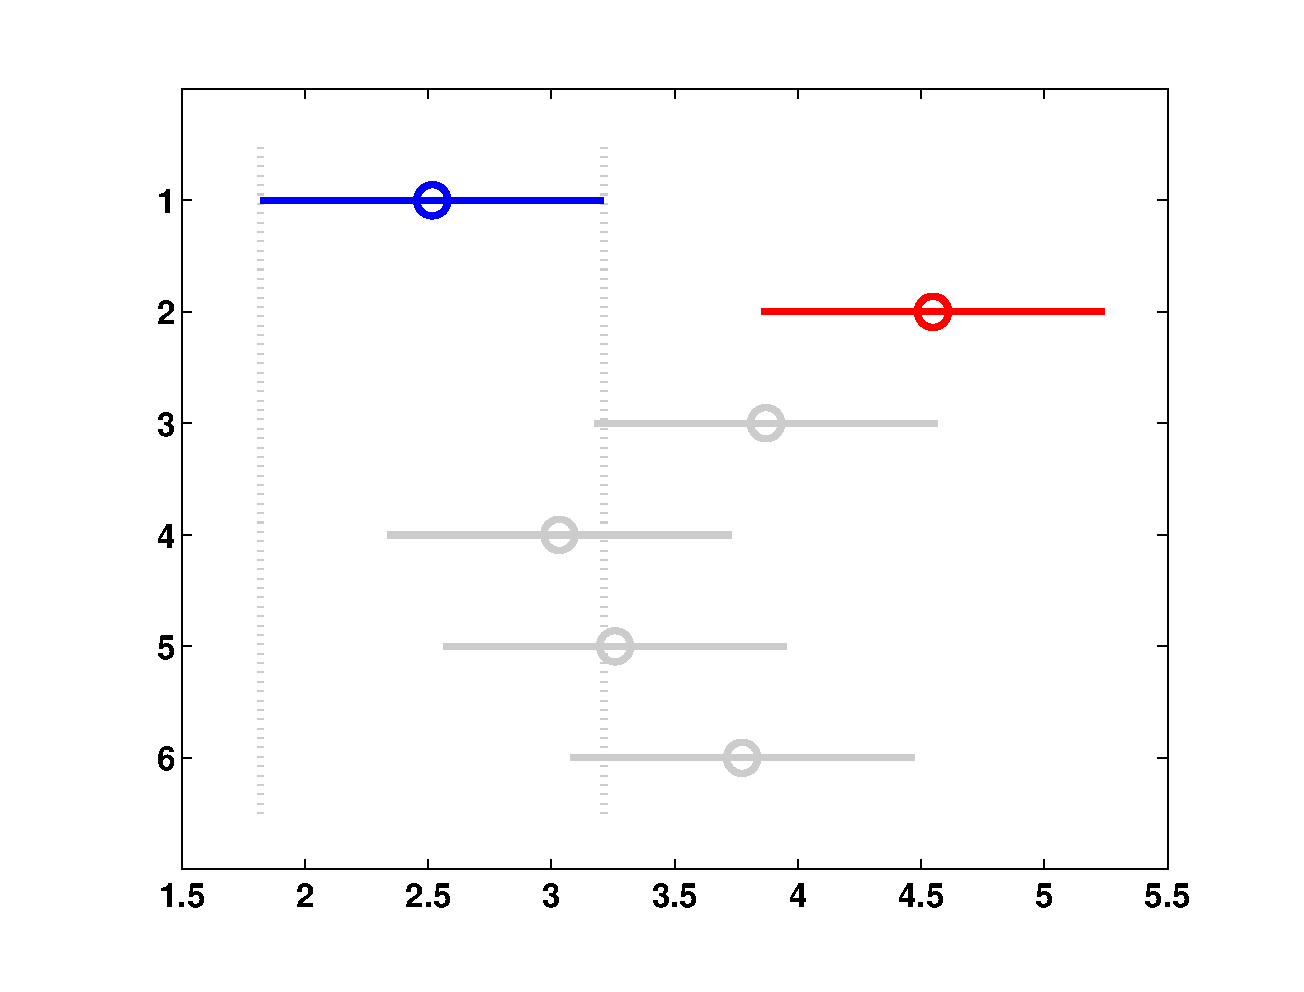
\includegraphics[width=\linewidth]{Figures/C-Bonferroni_HNMED_VS_ED5}
		\caption{GCE2} \label{fig:Bon_G2} 
	\end{subfigure}
	\begin{subfigure}[b]{0.49\linewidth}
		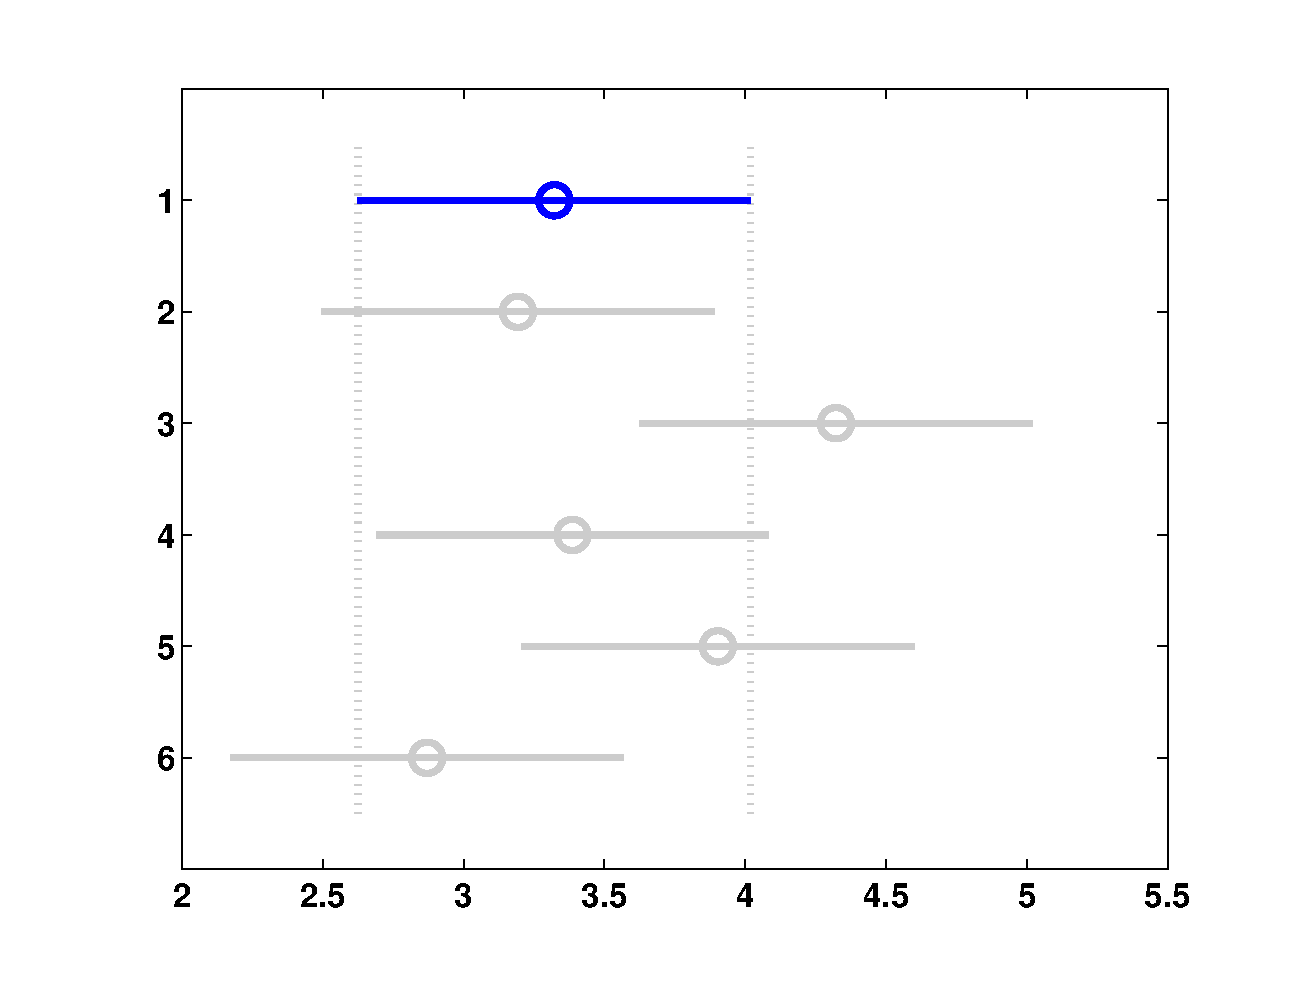
\includegraphics[width=\linewidth]{Figures/C-Bonferroni_HNMED_VS_ED6}
		\caption{SCE1} \label{fig:Bon_S1} 
	\end{subfigure}
	\caption[Resultados de las pruebas de Bonferroni-Dunn  obtenidos por las variantes HNMED vs ED/rand/1/bin en el Experimento C.]{Resultados de las pruebas de Bonferroni-Dunn  obtenidos por las variantes HNMED vs ED/rand/1/bin en el Experimento C. Se etiquetan en el eje vertical del 1 al 6 los algoritmos ED/rand/1/bin y HNMEDV1 a HNMEDV5   respectivamente.} \label{fig: Resultados de las pruebas de Bonferroni-Dunn para las variantes HNMED vs ED/rand/1/bin en el experimento C.} 
	
\end{figure}
\subsubsection{Observaciones}
Teniendo en cuenta los resultados obtenidos en ambos experimentos se pueden realizar las siguientes observaciones:
\begin{enumerate}
	\item Las variantes HNMED son capaces de encontrar resultados iguales o mejores para la mayoría de los problemas de optimización utilizando un número de evaluaciones menor, el cual representa un ahorro de más del 44\% en la mayoría de los problemas con excepción de MCE2 (-33.3\%) y SCE1 (-25.3\%) para las variante HNMED-V4 y V5).      
	\item De forma similar a los resultados obtenidos en el experimento A, las curvas de convergencia que describen las versiones de HNMED correspondientes a la mediana de las muestras se encuentran por debajo de la curva de la ED/ran/1/bin para la todos los problemas. Esto se logra reduciendo el número de símpleces y por tanto el tamaño de la población, esto implica un ahorro de evaluaciones por iteración y  permite realizar más operaciones de explotación. El hecho de que se alcancen los mínimos conocidos y valores de tendencia central competitivos descarta la posibilidad de que HNMED presente una tendencia a la convergencia prematura o estancamiento para los problemas presentados. 
	\item Al reducir el número de evaluaciones algunas versiones comienzan a presentar un desempeño significativamente inferior a la ED como es el caso de la V1. La variante HNMED-V5 es la que presenta mejor promedio de jerarquía en la mayoría de los problemas obteniendo resultados significativamente mejores o similares a la ED.
\end{enumerate}



%%%%%%%%%%%%%%%%%%%%%%%%%%%%%%%%%%%%%%%%%%%%%%%%%%%%%%%%%%%%%%%%%%%%%%%%%%%%%%%%%%%%%%%%%%%%%%%%%%%%%%%%%%%%%%%%%%%%

\section{Experimentos finales}
Los experimentos iniciales permitieron observar el comportamiento de las variantes HNMED diseñadas bajo el enfoque de hibridación propuesto en la Sección \ref{sec:Enfoque propuesto}. Se evidenció que a pesar de la rapidez de estos algoritmos, se presentaron dificultades en los problemas MCE1, MCE3 y GCE2. Estos problemas presentan un espacio de búsqueda más complejo, ya sea por presentar mayor número de restricciones, dimesionalidad, complejidad de la función objetivo o la cualquier combinación de estas características. 

Las variantes propuestas heredan, en cierta medida, algunas deficiencias del método de búsqueda local utilizado como la reducción del desempeño ante un aumento de la dimesionalidad del problema y la sensibilidad a los puntos iniciales. Por tanto, una mayor capacidad de exploración es requerida en orden de alcanzar mejores resultados. Con este objetivo trazado, se diseñó la HNMED-V6 cuyo desempeño es medido en los experimentos finales junto a la variante HNMED-V5.


\subsection{Experimentos D y E : Comparación de Variantes HNMED-V5 y HNMED-V6 con Algoritmo C-LSHADE}
El objetivo de ambos experimentos es comprobar la competitividad  de las dos mejores versiones HNMED. Por tanto, se realizan dos comparaciones finales por medio de estadística descriptiva e inferencial: el algoritmo HNMED-V5 y HNMED-V6 con el algoritmo C-LSHADE propuesto por Zapata en \cite{zapata_zapata_control_2017}, el cual es una variante competitiva del algoritmo DECV para el conjunto de problemas a resolver.
\subsubsection{Definición de medidas}
Se obtiene para cada algoritmo una muestra de $n=31$ ejecuciones. Para cada problema las observaciones en la muestra corresponden al valor de la función objetivo del mejor individuo factible encontrado por el algoritmo $A_i$en la ejecución $j$ para $j= \{ 1,2,...,n\}$. Se aplicarán al conjunto de muestras las siguientes pruebas de estadística descriptiva e inferencial:
\begin{enumerate}
	\item \textbf{Estadística descriptiva}: Se obtiene la la mejor y peor solución, mediana, promedio y desviación estándar de las muestras
	\item \textbf{Gráfica de convergencia}: Se presenta la gráfica de convergencia correspondiente a la mediana de la muestra para cada los dos algoritmo en comparación.
	\item \textbf{Prueba suma de Jerarquías de Wilcoxon}: con nivel significancia $\alpha=0.05$ para determinar si existen diferencias significativas entre el desempeño los dos algoritmos comparados. 
	
\end{enumerate}
\subsubsection{Planificación pre-experimental y configuración}
Para este experimento se mantuvo el número de evaluaciones realizadas por C-LSHADE según se describe en \cite{zapata_zapata_control_2017}. En la Tabla \ref{tab:Evaluaciones utilizadas por problema de optimización: Experimentos D y E.} se describe el número de evaluaciones realizadas por cada algoritmo comparado.

\begin{table}[]
	
	\caption{Evaluaciones utilizadas por problema de optimización: Experimentos D y E.}
	\label{tab:Evaluaciones utilizadas por problema de optimización: Experimentos D y E.}
	\centering
	
	\begin{tabular}{ccccccc}
		\textbf{Problema} &   C-LCHADE     &HNMED-V5&HNMED-V6 \\
		\hline
		MCE1   &   400000 &400000 &350000   \\
		MCE2   &   15000  &15000  &10000   \\
		MCE3   &   200000 &25000  &175000  \\
		GCE1   &   325000 &125000  &100000\\
		GCE2   &   150000 &225000  &125000\\
		SCE1   &   240000 &210000  &210000\\
	\end{tabular}
	
\end{table}
La configuración de parámetros utilizada por las variantes HNMED-V6:
\begin{enumerate}
	\item Se establece la probabilidad de cruza $CR=\{0.8, 1\}$ para ED y HNMED para todos los problemas.
	\item Se establece el factor de escala $F=\{0.3, 0.9\}$ para ED y HNMED para todos los problemas.
	\item Para la variante HNMEDV5 establecieron los parámetros de reflexión $\alpha=2$, expansión $\gamma=1.7$ $\beta=0.3$ para todos los problemas.
	\item El tamaño de población utilizado se ajusta para cada algoritmo según la Tabla \ref{tab:Tamaños de población utilizados para cada problema en los experimentos finales}. 
\end{enumerate}

\begin{table}[]
	\centering
	\caption{Tamaños de población utilizados para cada problema en los experimentos finales.}
	\label{tab:Tamaños de población utilizados para cada problema en los experimentos finales}
	
	\begin{tabular}{cccccccccccc}
		& \textbf{C-LSHADE } & \multicolumn{2}{l}{\textbf{HNMED-V5}}&\multicolumn{2}{l}{\textbf{HNMED-V6}}\\
		\hline
		\textbf{Problema} & \textbf{NP}    & \textbf{NS} & \textbf{NP}& \textbf{NS}& \textbf{NP}\\
		\hline
		MCE1     & 138           & 9           & 144 &8&128   \\
		MCE2     & 50            & 3           & 21  &4&28       \\
		MCE3     & 138           & 7           & 140 &5&75      \\
		GCE1     & 138           & 9           & 135 &7&105        \\
		GCE2     & 138           & 9           & 135 &7&105    \\
		SCE1     & 50            & 7           & 35  &2&10       
	\end{tabular}
	
\end{table}


\subsubsection{Resultados del Experimento D}
La Tabla \ref{tab:Resultados estadísticos obtenidos por HNMED-V5 y el algoritmo C-LSHADE en los seis problemas de diseño mecatrónico} muestra los resultados estadísticos obtenidos por HNMED-V5 y los obtenidos por C-LSHADE en \cite{zapata_zapata_control_2017}. En la Figura \ref{fig: Gráficas de convergencia obtenidas por HNMED-V5 y CLSHADE para el Experimento D} se presentan las gráficas de convergencias correspondientes al Experimento D para los seis problemas. Finalmente, la Tabla \ref{tab:Wilcoxon HNMED-V5-CLSHADE} contiene los resultados de la prueba de Suma de Jerarquías de Wilcoxon con un nivel de significancia de 95\%.
%%%%%%%%%%%%%%%%%%%%%%%%%%%%%%%%%%%%%%%%%%%%%%%%%%%%%%%%%%%%%%%%%%%%%%%%%%%%%%%%%%%%%%%%%%%%%%%%%%%

\begin{table}
	\centering
	\caption[Resultados estadísticos obtenidos por HNMED-V5 y C-LSHADE
	 en el Experimento D para los seis problemas de diseño mecatrónico.]{Resultados estadísticos obtenidos por HNMED-V5 y C-LSHADE
	 	en el Experimento D para los seis problemas de diseño mecatrónico. Se marcan en negritas los
		mejores valores de cada medida.}\label{tab:Resultados estadísticos obtenidos por HNMED-V5 y el algoritmo C-LSHADE en los seis problemas de diseño mecatrónico}
	\begin{tabular}{clcc} 
		\hline
		Problema              & Estadística   & HNMED-V5 & C-LSHADE  \\ 
		\hline
		\multirow{6}{*}{MCE1} & Mejor        & 6.3108E-29 & \textbf{0 }      \\
		& Peor         &2.7323E-02&  \textbf{6.4277E-04}  \\
		& Mediana      &3.2843E-04&\textbf{3.6143E-08}     \\
		& Promedio     &2.5730E-03& \textbf{ 2.4021E-04 } \\
		& Desv. Est.   &6.9657E-03&\textbf{ 2.7680E-04}\\
		& Evaluaciones &400000   &  400000       \\
		\hline
		\multirow{6}{*}{MCE2} & Mejor        &2.6280E-03&2.6280E-03
		\\
		& Peor         &\textbf{2.6280E-03}&2.6281E-03                \\
		& Mediana      &2.6280E-03&2.6280E-03   \\
		& Promedio     &2.6280E-03&2.6280E-03    \\
		& Desv. Est.   &\textbf{2.1708E-10}&8.5532E-09 \\
		& Evaluaciones &15000&15000                \\
		\hline
		\multirow{6}{*}{MCE3} & Mejor        &2.7577E-01&\textbf{2.7496E-01}  \\
		& Peor         &1.3508E+01&1.3508E+01     \\
		& Mediana      &5.0946E-01&\textbf{2.8886E-01} \\
		& Promedio     &4.8813E+00&\textbf{1.6068E+00}\\
		& Desv. Est.   &6.2202E+00&\textbf{3.9629E+00}\\
		& Evaluaciones &225000& \textbf{200000} (-12.5\%) \\
		\hline
		\multirow{6}{*}{GCE1} & Mejor        &0&0\\
		& Peor         &7.6992E-28&\textbf{3.0292E-28}\\
		& Mediana      &1.8932E-29&\textbf{1.2621E-29}\\
		& Promedio     &1.0886E-28&\textbf{2.7991E-28} \\
		& Desv. Est.   &1.7494E-28&\textbf{5.6901E-29}\\
		& Evaluaciones &\textbf{125000}(-61.5\%)&325000 \\
		\hline
		\multirow{6}{*}{GCE2} & Mejor        &1.1385E-01&1.1385E-01\\
		& Peor         &1.6276E-01&\textbf{1.5783E-01}\\
		& Mediana      &1.1631E-01&\textbf{1.1392E-01 }\\
		& Promedio     &1.2887E-01&\textbf{1.2066E-01  }\\
		& Desv. Est.   &1.9809E-02&\textbf{1.5457E-02 }\\
		& Evaluaciones &250000&\textbf{150000}(-40.0\%) \\
		\hline
		
		
		\multirow{6}{*}{SCE1} & Mejor        &\textbf{-5.3652E+05}&-5.3205E+05 \\
		& Peor         &-5.3080E+05&-5.3205E+05\\
		& Mediana      &\textbf{-5.3217E+05}&-5.3205E+05\\
		& Promedio     &\textbf{5.3230E+05}&-5.3205E+05\\
		& Desv. Est.   &1.094E+03&\textbf{1.0515E-04}\\
		& Evaluaciones &\textbf{216000}(-10.0\%)&240000 \\
		
		
		\hline
	\end{tabular}
\end{table}


\begin{figure}
	\centering
	\begin{subfigure}[b]{0.49\linewidth}
		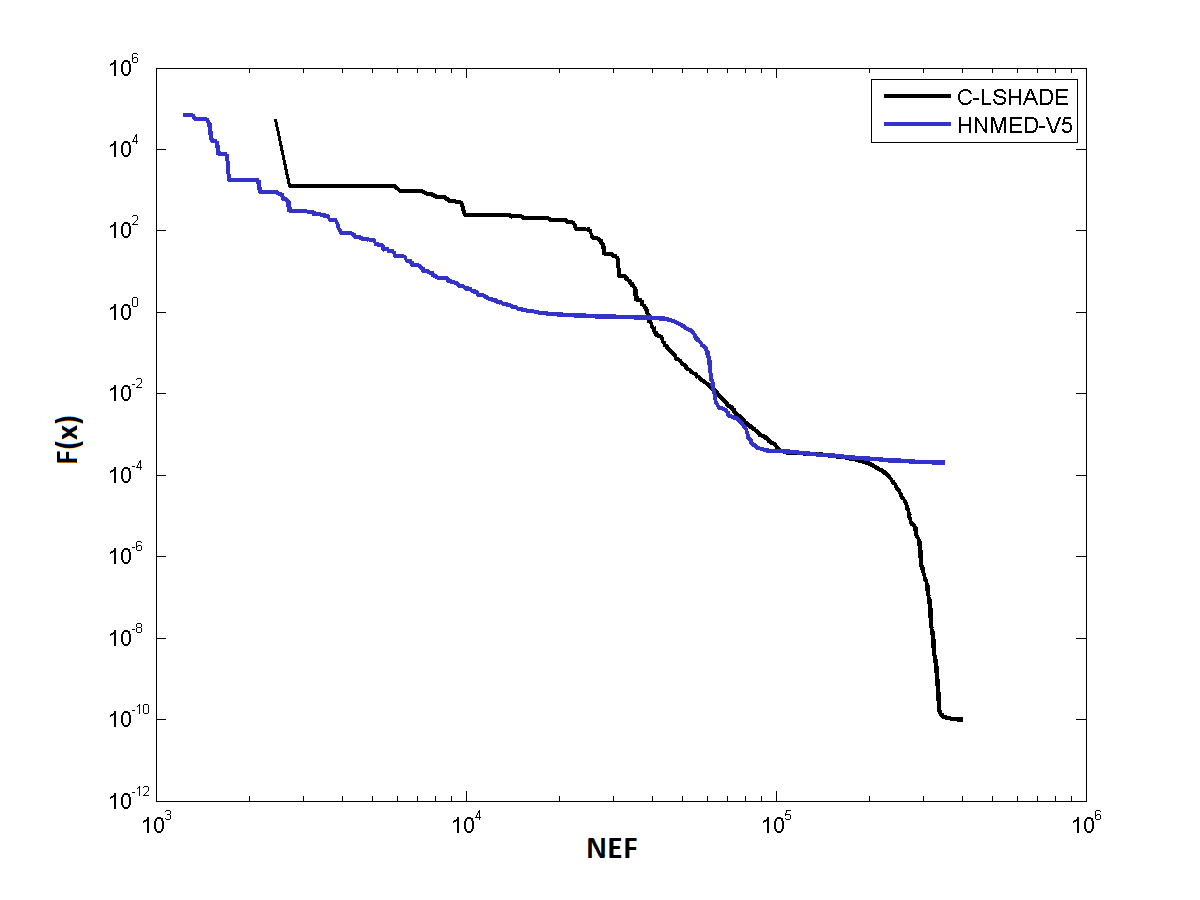
\includegraphics[width=\linewidth]{Figures/D-Grafica_Convergencia_Problema_1}
		\caption{MCE1} \label{fig:M1} 
	\end{subfigure}
	\begin{subfigure}[b]{0.49\linewidth}
		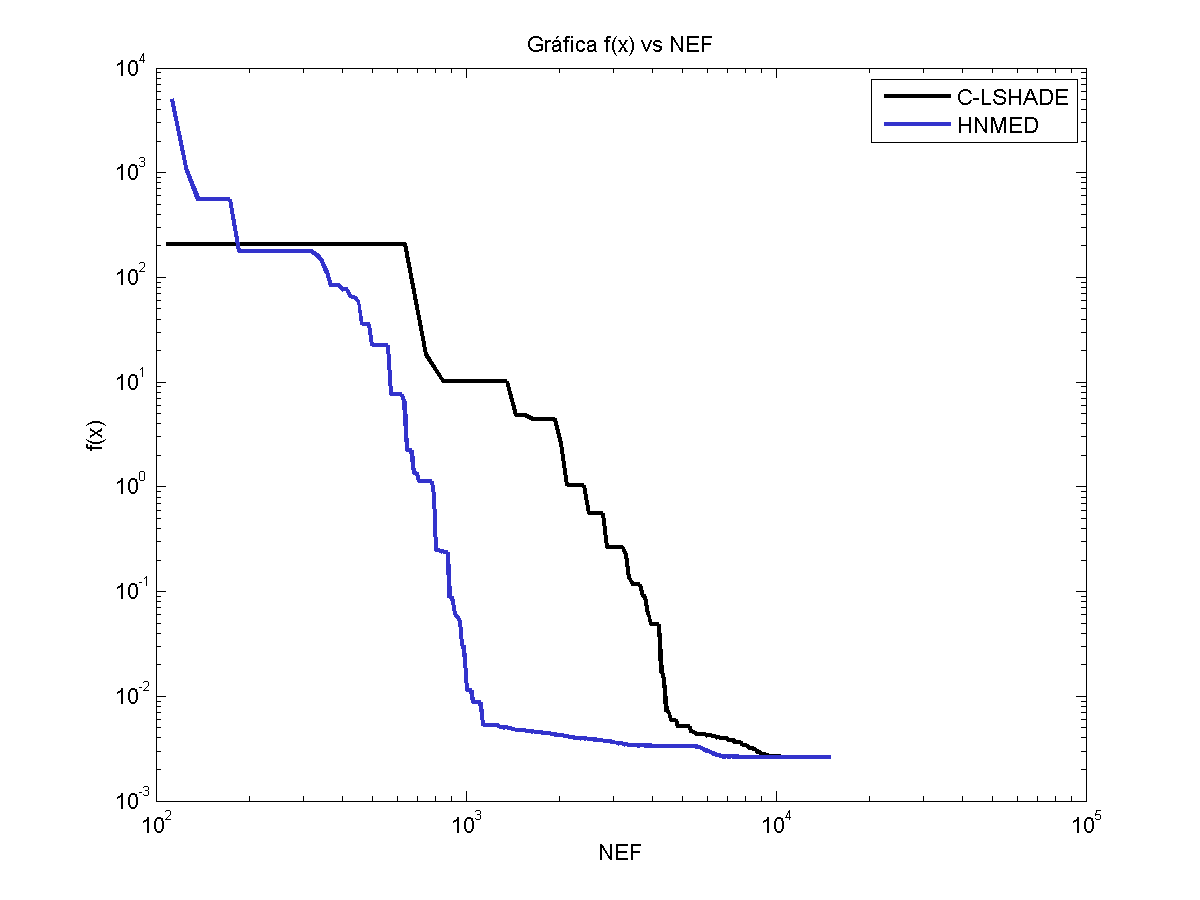
\includegraphics[width=\textwidth]{Figures/D-Grafica_Convergencia_Problema_2}
		\caption{MCE2} \label{fig:M2} 
	\end{subfigure}
	\begin{subfigure}[b]{0.49\linewidth}
		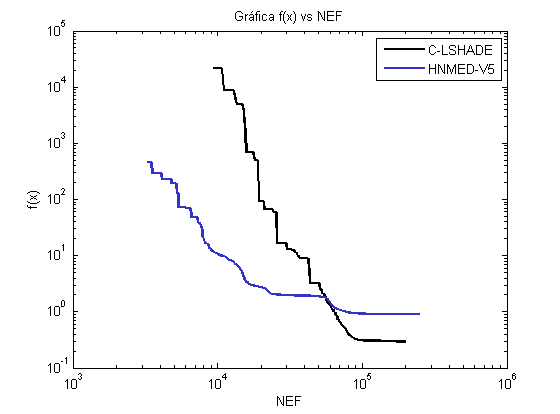
\includegraphics[width=\linewidth]{Figures/D-Grafica_Convergencia_Problema_3}
		\caption{MCE3} \label{fig:M3} 
	\end{subfigure}
	\begin{subfigure}[b]{0.49\linewidth}
		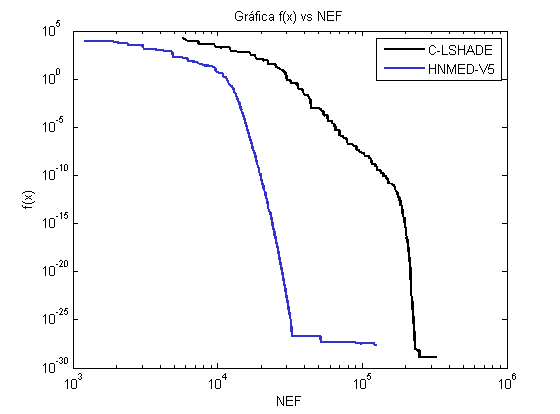
\includegraphics[width=\linewidth]{Figures/D-Grafica_Convergencia_Problema_4}
		\caption{GCE1} \label{fig:G1} 
	\end{subfigure}
	\begin{subfigure}[b]{0.49\linewidth}
		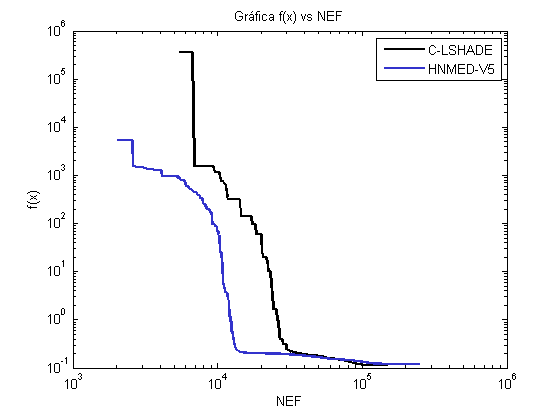
\includegraphics[width=\linewidth]{Figures/D-Grafica_Convergencia_Problema_5}
		\caption{GCE2} \label{fig:G2} 
	\end{subfigure}
	\begin{subfigure}[b]{0.49\linewidth}
		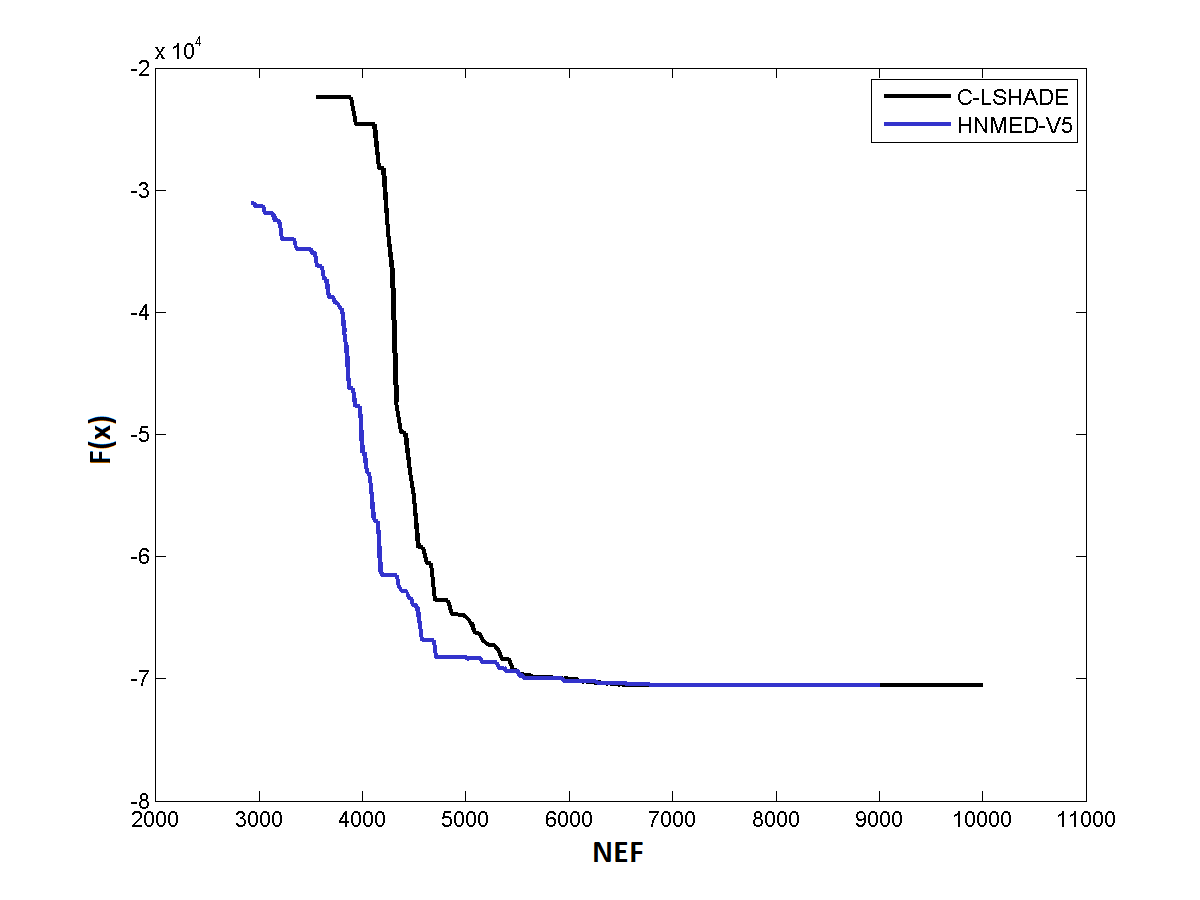
\includegraphics[width=\linewidth]{Figures/D-Grafica_Convergencia_Problema_6}
		\caption{SCE2} \label{fig:S1} 
	\end{subfigure}
	\caption[Gráficas de convergencia obtenidas por la variante HNMED-V5 y C-LSHADE en el Experimento D.]{Gráficas de convergencia obtenidas por la variante HNMED y C-LSHADE en el Experimento D. El eje horizontal presenta el número de evaluaciones de la función objetivo (NEF) y el eje vertical el valor de  $f(x)$.} \label{fig: Gráficas de convergencia obtenidas por HNMED-V5 y CLSHADE para el Experimento D} 
	
\end{figure}

\begin{table}
	\centering
	\caption[Comparación de C-LSHADE y HNMED-V5 en los seis problemas de optimización mediante la prueba de Suma de Jerarquías de Wilcoxon.]{Comparación de C-LSHADE y HNMED-V5 en los seis problemas de optimización mediante la prueba de Suma de Jerarquías de Wilcoxon. Los símbolos +, - y $\approx$ señalan que HNMED-V5 obtuvo un desempeño significativamente mejor (+), significativamente peor (-) o no significativamente diferente ($\approx$) comparado contra C-LSHADE usando la prueba de suma de jerarquías de Wilcoxon con un 95 \% de confianza} \label{tab:Wilcoxon HNMED-V5-CLSHADE}
	\begin{tabular}{cccccccc}
		\multirow{2}{*}{\textbf{vs C-LSHADE}} & \multicolumn{6}{c}{\textbf{Problemas}}           & \textbf{Total}  \\
		& MCE1 & MCE2 & MCE3 & GCE1 & GCE2 & SCE1 &        \\
		\hline
		\multirow{3}{*}{HNMED-V5}    &      &  $+$    &      &      &       & $ +$    &  2      \\
		&   $-$  &      &  $ -$   &      &  $ - $  &       & 3       \\
		&      &      &       &$\approx$ &  &        &    1
	\end{tabular}
\end{table}
%%%%%%%%%%%%%%%%%%%%%%%%%%%%%%%%%%%%%%%%%%%%%%%%%%%%%%%%%%%%%%%%%%%%%%%%%%%%%%%%%%%%%%%%%%%%%%%%%%%


\subsubsection{Resultados del Experimento E}
Las Tablas \ref{tab:Resultados estadísticos obtenidos por variantes HNMED6 y ED  en experimento E.} y \ref{tab:Resultados estadísticos obtenidos por variantes HNMED6 y CLSHADE  en experimento E.} se muestran los resultados estadísticos obtenidos por la HNMED-V6 frente a la ED/rand/1/bin y C-LSHADE respectivamente. Se agrega la comparación estadística de HNMED-V6 con la ED/rand/1/bin para evidenciar la reducción del número evaluaciones. En la Figura \ref{fig: Gráficas de convergencia obtenidas por HNMED-V6 y CLSHADE para el Experimento E.} se muestran las gráficas de convergencia correspondientes al Experimento E. En la Tabla \ref{tab:Wilcoxon HNMED-V6-CLSHADE} se presenta para la comparación de HNMED-V6 y C-LSHADE mediante prueba de suma de jerarquías de Wilcoxon.  

\begin{table}
	\centering
	\caption[Resultados estadísticos obtenidos por HNMED-V6 vs ED/rand/1/bin en el experimento E
		para los seis problemas de diseño mecatrónico.]{Resultados estadísticos obtenidos por HNMED-V6 vs ED/rand/1/bin en el experimento E
		para los seis problemas de diseño mecatrónico. Se marcan en negritas los
		mejores valores de cada medida.} \label{tab:Resultados estadísticos obtenidos por variantes HNMED6 y ED  en experimento E.}
	\begin{tabular}{clcc} 
		\hline
		Problema              & Estadística  & HNMED-V5 & ED/rand/1/bin  \\ 
		\hline
		\multirow{6}{*}{MCE1} & Mejor        & \textbf{3.7865E-29} &1.7670E-28          \\
		& Peor         &\textbf{3.6342E-03}&2.7649E-02
		\\
		& Mediana      &\textbf{6.5633E-28}&4.2746E-06            \\
		& Promedio     &\textbf{1.6110E-04}&2.9850E-01            \\
		& Desv. Est.   &\textbf{6.4886E-04}& 8.1906E-03
		\\
		& Evaluaciones &\textbf{350000}(-53.53\%)  &  750030       \\
		\hline
		
		\multirow{6}{*}{MCE2} & Mejor        &\textbf{2.5643E-04}&2.6280E-03
		\\
		& Peor         &\textbf{2.6280E-03}&2.6426E-03  \\
		& Mediana      &2.6280E-03&2.6280E-03   \\
		& Promedio     &\textbf{2.3985E-03}&2.6288E-03   \\
		& Desv. Est.   &7.1276E-04&\textbf{2.7205E-06} \\
		& Evaluaciones &\textbf{10000}(50.0\%) &20000                \\
		\hline
		
		\multirow{6}{*}{MCE3} & Mejor        &2.7496E-01&2.7496E-01  \\
		& Peor         &1.3508E+01&1.3508E+01     \\
		& Mediana      &3.0867E-01&\textbf{2.7563E-01} \\
		& Promedio     &2.4412E+00&\textbf{1.2313E+00}\\
		& Desv. Est.   &4.7466E+00&\textbf{3.2919E+00}\\
		& Evaluaciones &\textbf{175000}(-61.1\%)& 450018 \\
		\hline
		\multirow{6}{*}{GCE1} & Mejor        &\textbf{0}&6.7147E-27\\
		& Peor         &\textbf{5.3327E-28}&5.9926E-20\\
		& Mediana      &\textbf{1.2621E-29}&3.9485E-23\\
		& Promedio     &\textbf{5.8223E-29}&3.4957E-21\\
		& Desv. Est.   &\textbf{1.1714E-28}&1.2077E-20\\
		& Evaluaciones &\textbf{100000}(-86.6\%)&750030 \\
		\hline
		
		
		\multirow{6}{*}{GCE2} & Mejor        &1.1385E-01&1.1385E-01\\
		& Peor         &2.3331E-01&\textbf{1.6075E-01}\\
		& Mediana      &1.5210E-01&\textbf{1.1447E-01 }\\
		& Promedio     &1.4351E-01&\textbf{1.2080E-01  }\\
		& Desv. Est.   &3.3531E-02&\textbf{1.4713E-02 }\\
		& Evaluaciones &\textbf{125000}(-72.2\%)&450018 \\
		\hline
		\multirow{6}{*}{SCE1} & Mejor        &\textbf{ -5.5147E+05}&-5.3206E+05 \\
		& Peor         &\textbf{ -5.5147E+05}&-5.3204E+05\\
		& Mediana      &\textbf{ -5.5147E+05}&-5.3205E+05\\
		& Promedio     & \textbf{-5.5147E+05}&-5.3205E+05\\
		& Desv. Est.   &\textbf{2.3667E-10}&3.3010E+00\\
		& Evaluaciones &\textbf{216000}(-25.0\%)&288000 \\
		
		
		\hline
	\end{tabular}
\end{table}

\begin{table}
	\centering
	\caption[Resultados estadísticos obtenidos por HNMED-V6 vs C-LSHADE
	en los seis problemas de diseño mecatrónico]{Resultados estadísticos obtenidos por HNMED-V6 vs C-LSHADE
		en los seis problemas de diseño mecatrónico. Se marcan en negritas los
		mejores valores de cada medida.} \label{tab:Resultados estadísticos obtenidos por variantes HNMED6 y CLSHADE  en experimento E.}
	\begin{tabular}{clcc} 
		\hline
		Problema              & Estadística   & HNMED-V6 & C-LSHADE  \\ 
		\hline
		\multirow{6}{*}{MCE1} & Mejor        & 3.7865E-29 &\textbf{ 0 }            \\
		& Peor         &3.6342E-03&  \textbf{6.4277E-04}
		\\
		& Mediana      &\textbf{6.56332E-28}&3.6143E-08            \\
		& Promedio     &\textbf{1.6110E-04}&  2.4021E-04             \\
		& Desv. Est.   &6.4886E-04& \textbf{2.7680E-04 }         \\
		& Evaluaciones &\textbf{350000}(-12.5\%)  &  400000       \\
		\hline
		
		\multirow{6}{*}{MCE2} & Mejor        &\textbf{2.5643E-04}&2.6280E-03
		\\
		& Peor         &\textbf{2.6280E-03}&2.6281E-03                \\
		& Mediana      &2.6280E-03&2.6280E-03   \\
		& Promedio     &\textbf{2.3985E-03}&2.6280E-03    \\
		& Desv. Est.   &7.1276E-04&\textbf{8.5532E-09} \\
		& Evaluaciones &\textbf{10000}(30.0\%) &15000                \\
		\hline
		
		\multirow{6}{*}{MCE3} & Mejor        &2.7496E-01&2.7496E-01  \\
		& Peor         &1.3508E+01&1.3508E+01     \\
		& Mediana      &3.0867E-01&\textbf{2.8886E-01} \\
		& Promedio     &2.4412E+00&\textbf{1.6068E+00}\\
		& Desv. Est.   &4.7466E+00&\textbf{3.9629E+00}\\
		& Evaluaciones &\textbf{175000}(-22.2\%)& 200000 \\
		\hline
		\multirow{6}{*}{GCE1} & Mejor        &0&0\\
		& Peor         &5.3327E-28&\textbf{3.0292E-28}\\
		& Mediana      &1.2621E-29&1.2621E-29\\
		& Promedio     &\textbf{5.8223E-29}&2.7991E-28 \\
		& Desv. Est.   &1.1714E-28&\textbf{5.6901E-29}\\
		& Evaluaciones &\textbf{100000}(-61.5\%)&325000 \\
		\hline
		
		
		\multirow{6}{*}{GCE2} & Mejor        &1.1385E-01&1.1385E-01\\
		& Peor         &2.3331E-01&\textbf{1.5783E-01}\\
		& Mediana      &1.5210E-01&\textbf{1.1392E-01 }\\
		& Promedio     &1.4351E-01&\textbf{1.2066E-01  }\\
		& Desv. Est.   &3.3531E-02&\textbf{1.5457E-02 }\\
		& Evaluaciones &\textbf{125000}(-16.6\%)&150000 \\
		\hline
		\multirow{6}{*}{SCE1} & Mejor        &\textbf{ -5.5147E+05}&-5.3205E+05 \\
		& Peor         &\textbf{ -5.5147E+05}&-5.3205E+05\\
		& Mediana      &\textbf{ -5.5147E+05}&-5.3205E+05\\
		& Promedio     & \textbf{-5.5147E+05}&-5.3205E+05\\
		& Desv. Est.   &\textbf{2.3667E-10}&1.0515E-04\\
		& Evaluaciones &\textbf{216000}(-12.5\%)&240000 \\
		
		
		\hline
	\end{tabular}
\end{table}


\begin{figure}
	\centering
	\begin{subfigure}[b]{0.49\linewidth}
		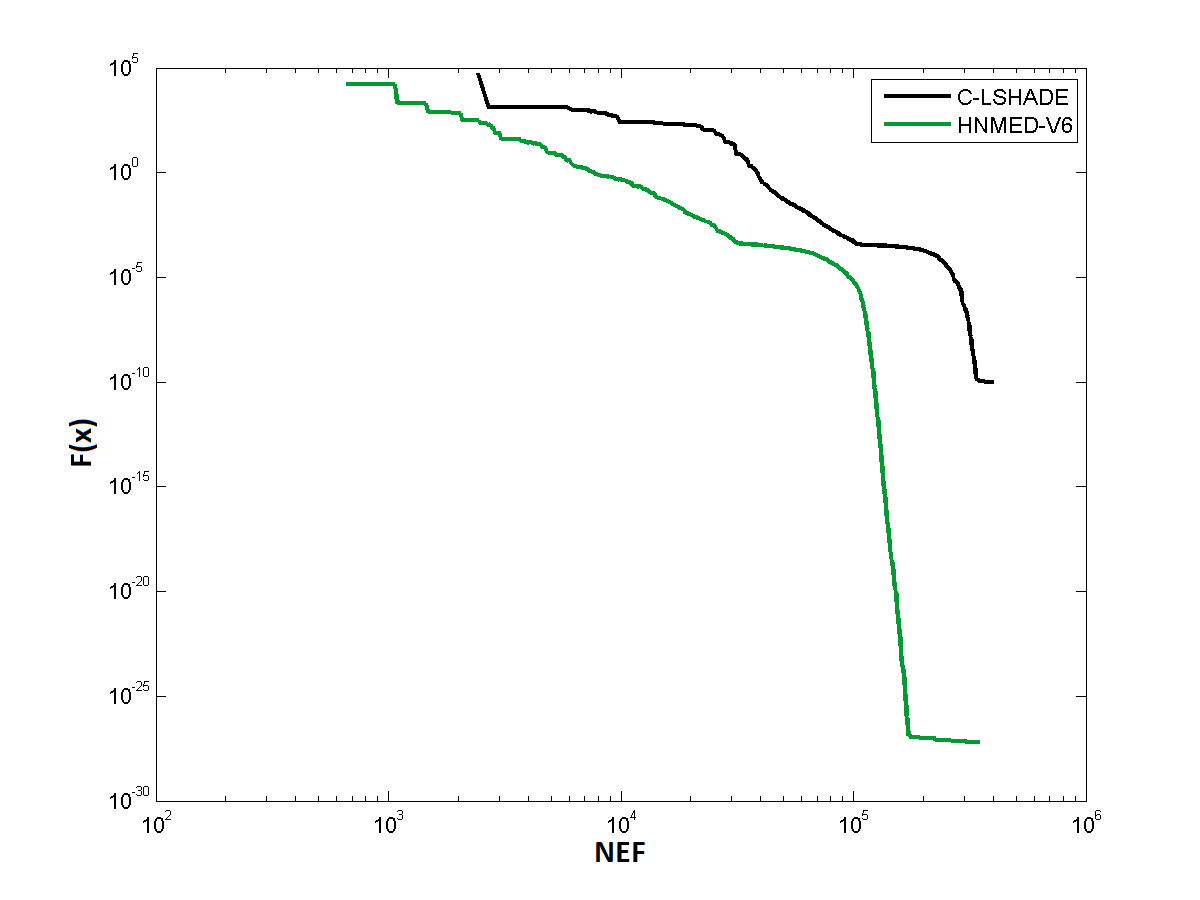
\includegraphics[width=\linewidth]{Figures/E-Grafica_Convergencia_Problema_1}
		\caption{MCE1} \label{fig:M1} 
	\end{subfigure}
	\begin{subfigure}[b]{0.49\linewidth}
		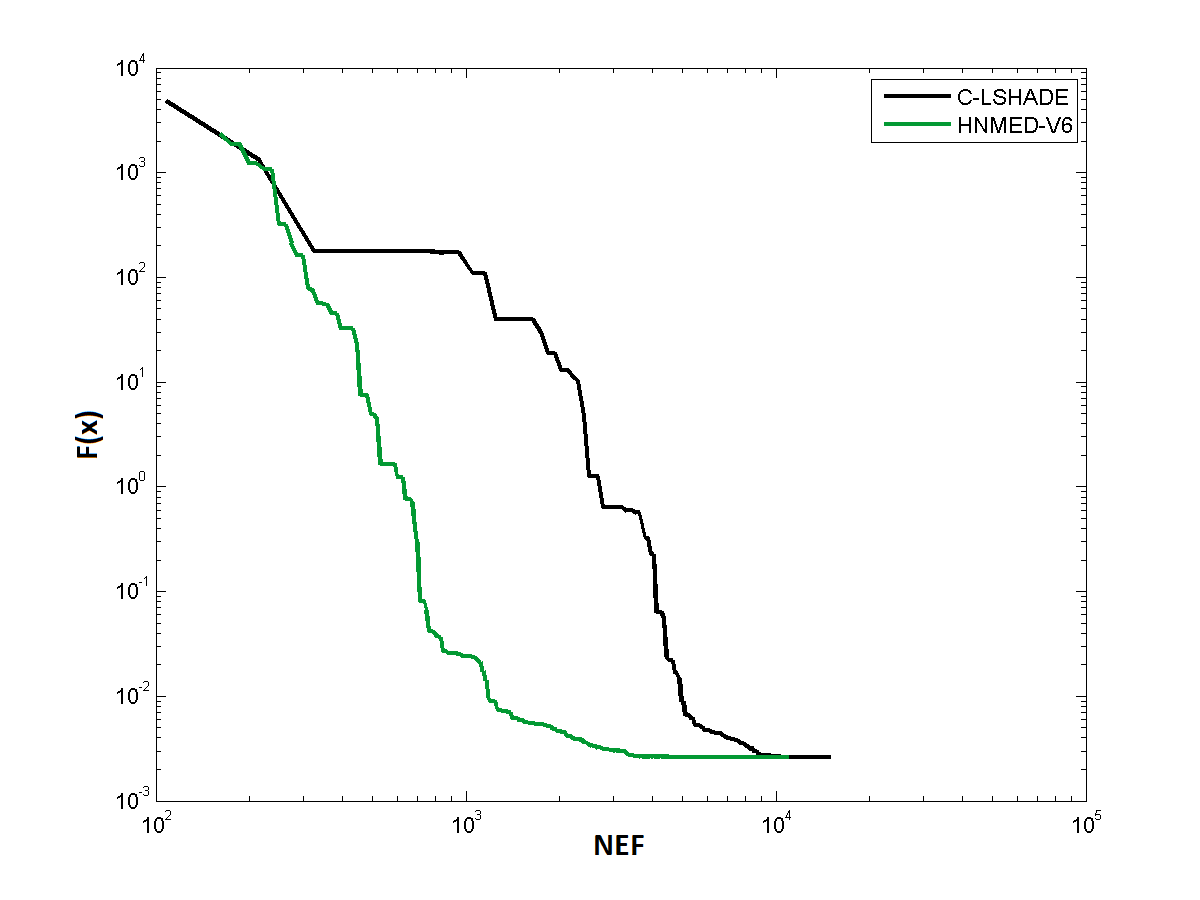
\includegraphics[width=\textwidth]{Figures/E-Grafica_Convergencia_Problema_2}
		\caption{MCE2} \label{fig:M2} 
	\end{subfigure}
	\begin{subfigure}[b]{0.49\linewidth}
		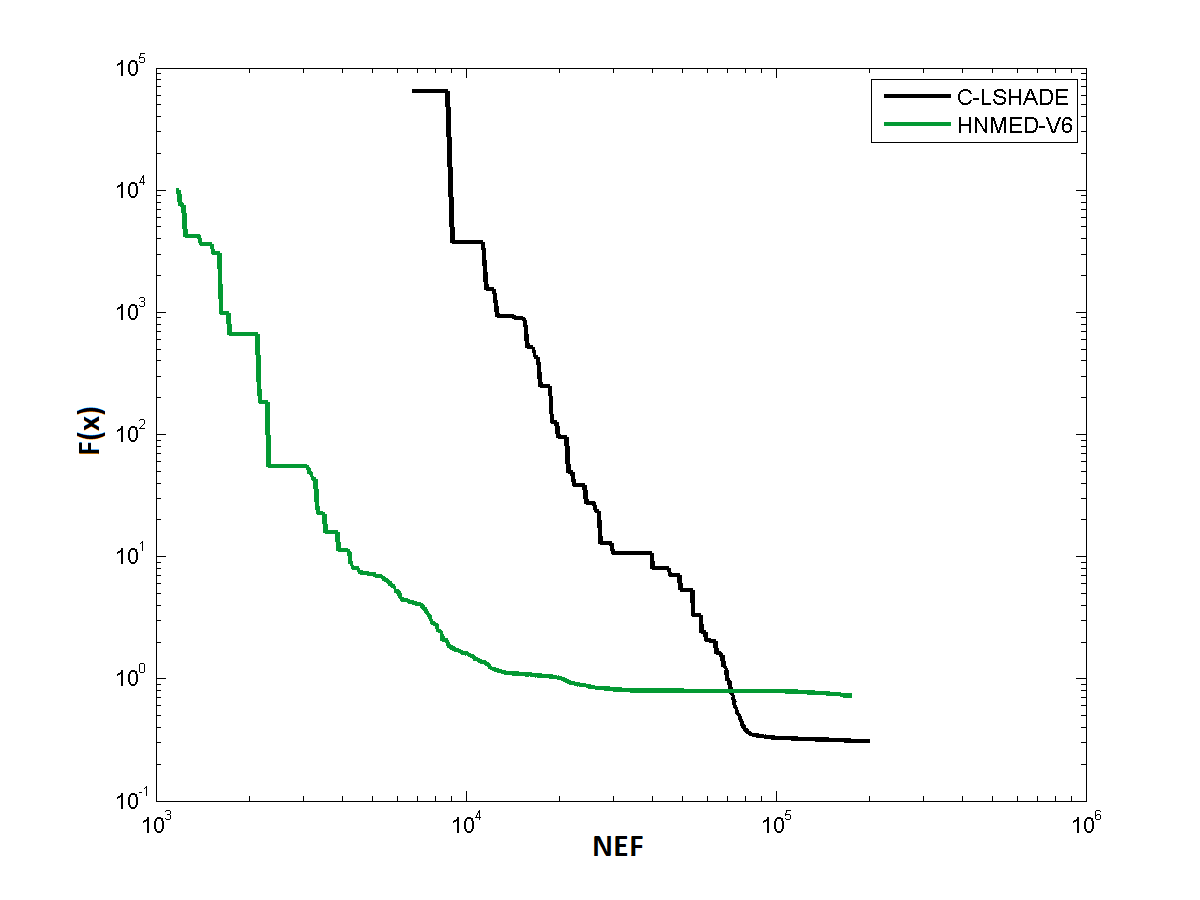
\includegraphics[width=\linewidth]{Figures/E-Grafica_Convergencia_Problema_3}
		\caption{MCE3} \label{fig:M3} 
	\end{subfigure}
	\begin{subfigure}[b]{0.49\linewidth}
		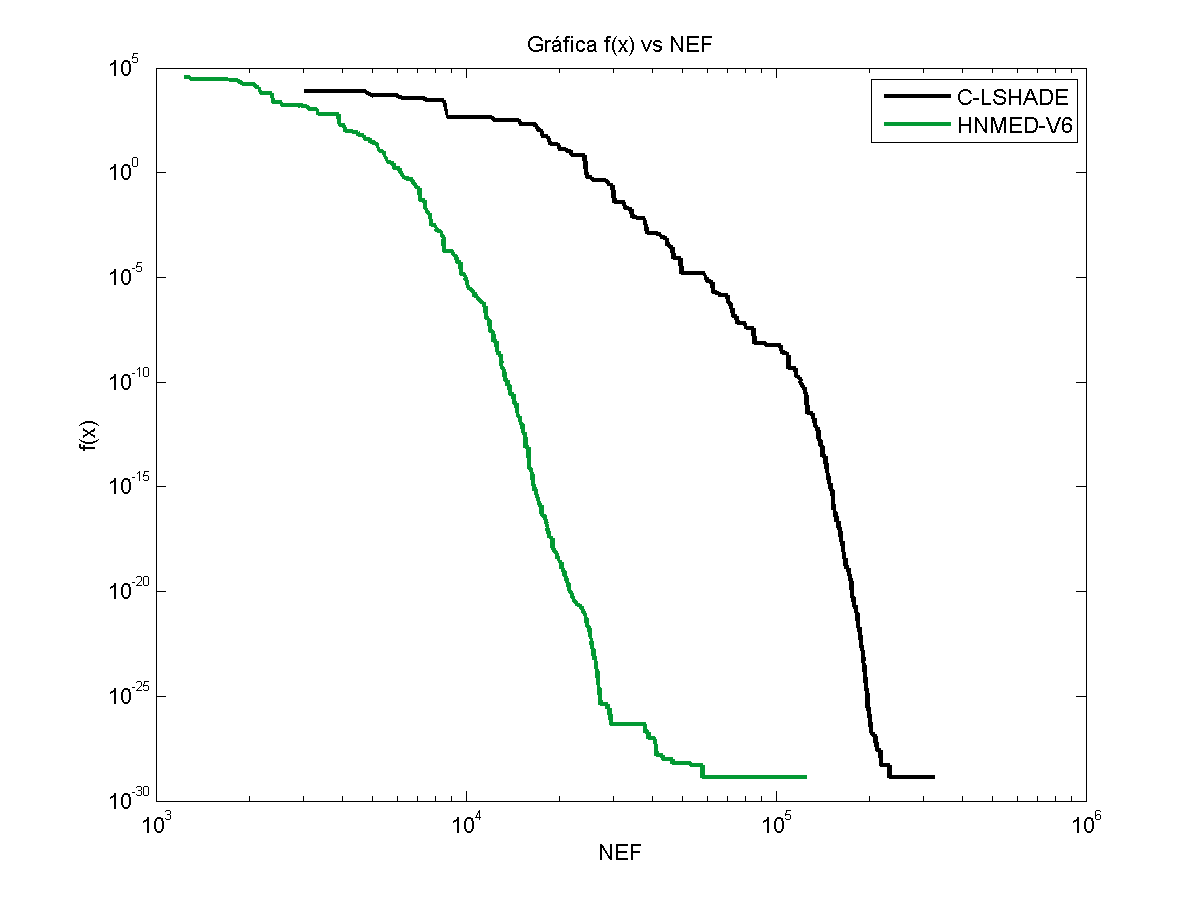
\includegraphics[width=\linewidth]{Figures/E-Grafica_Convergencia_Problema_4}
		\caption{GCE1} \label{fig:G1} 
	\end{subfigure}
	\begin{subfigure}[b]{0.49\linewidth}
		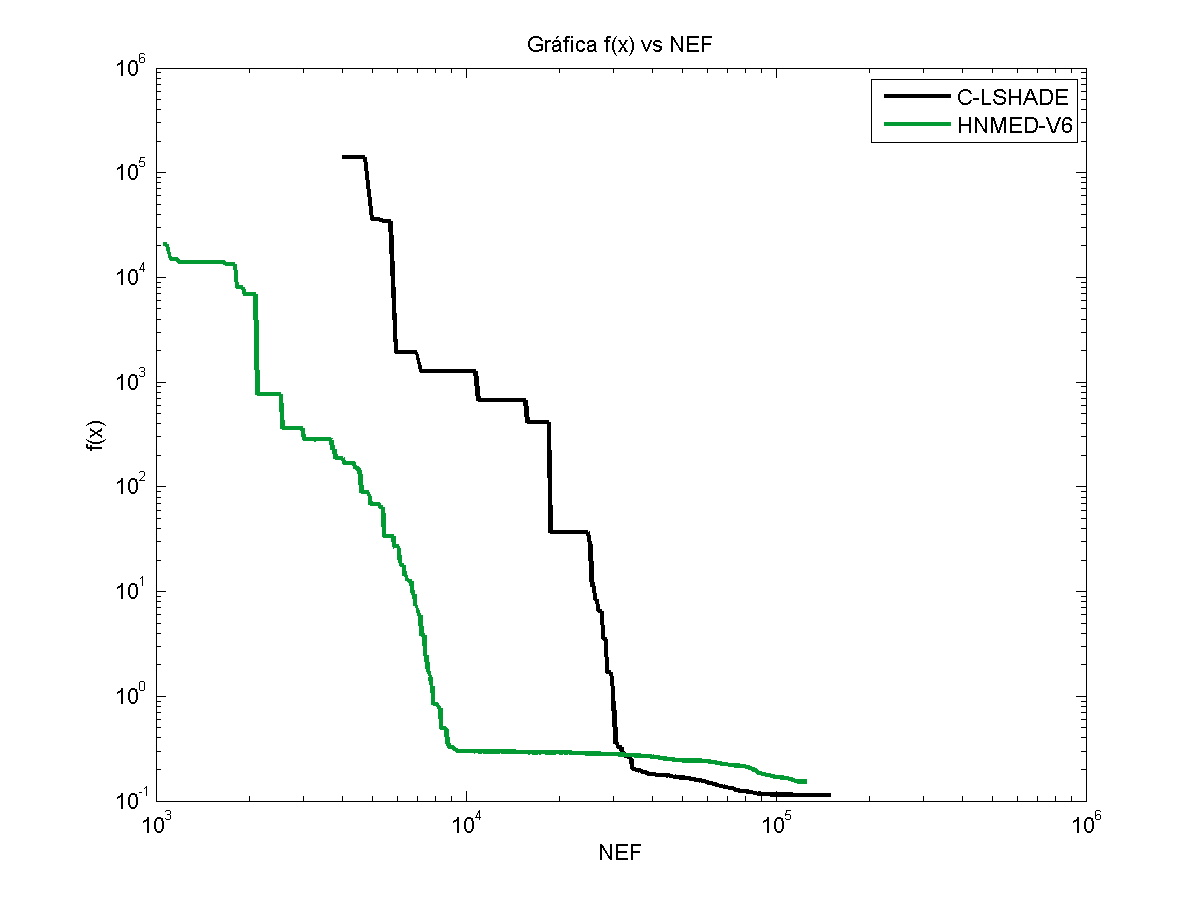
\includegraphics[width=\linewidth]{Figures/E-Grafica_Convergencia_Problema_5}
		\caption{GCE2} \label{fig:G2} 
	\end{subfigure}
	\begin{subfigure}[b]{0.49\linewidth}
		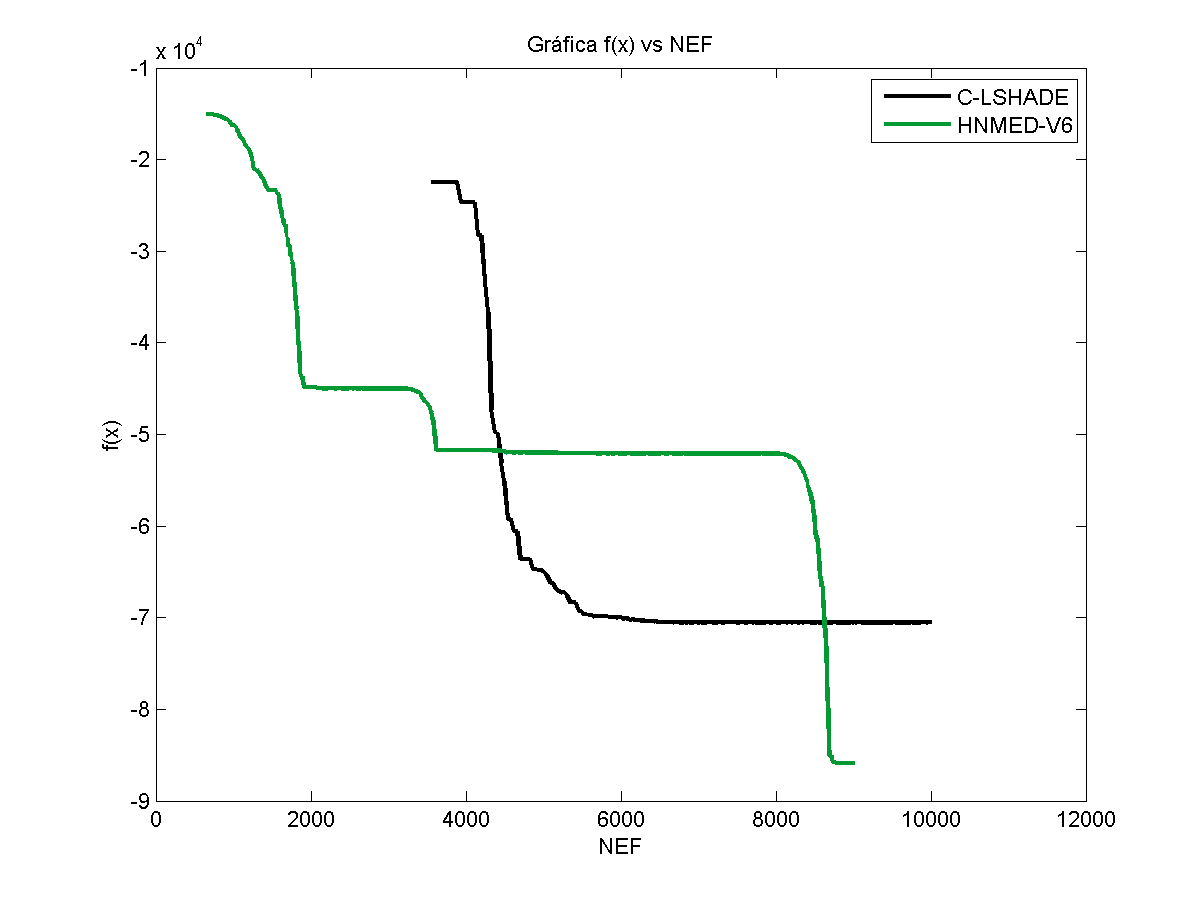
\includegraphics[width=\linewidth]{Figures/E-Grafica_Convergencia_Problema_6}
		\caption{SCE2} \label{fig:S1} 
	\end{subfigure}
	\caption[Gráficas de convergencia obtenidas por la variante HNMED-V6 y C-LSHADE en el Experimento E.]{Gráficas de convergencia obtenidas por la variante HNMED-V6 y C-LSHADE en el Experimento E. El eje horizontal presenta el número de evaluaciones de la función objetivo (NEF) y el eje vertical el valor de  $f(x)$.} \label{fig: Gráficas de convergencia obtenidas por HNMED-V6 y CLSHADE para el Experimento E.} 
	
\end{figure}


\begin{table}
	\centering
	\caption[Comparación de C-LSHADE y HNMED-V6 en los seis problemas de optimización mediante la prueba de Suma de Jerarquías de Wilcoxon.]{Comparación de C-LSHADE y HNMED-V6 en los seis problemas de optimización mediante la prueba de Suma de Jerarquías de Wilcoxon. Los símbolos +, - y $\approx$ señalan que HNMED-V6 obtuvo un desempeño significativamente mejor (+), significativamente peor (-) o no significativamente diferente ($\approx$) comparado contra LSHADE-CV usando la prueba de suma de jerarquías de Wilcoxon con un 95 \% de confianza} \label{tab:Wilcoxon HNMED-V6-CLSHADE}
	\begin{tabular}{cccccccc}
		\multirow{2}{*}{\textbf{vs C-LSHADE}} & \multicolumn{6}{c}{\textbf{Problemas}}           & \textbf{Total}  \\
	                                        	& MCE1 & MCE2 & MCE3 & GCE1 & GCE2 & SCE1 &        \\
		\hline
		\multirow{3}{*}{HNMED-V6}    &      &  $+$    &      &      &      &  $+$    &   2     \\
		&      &      & $-$     &      &    $-$  &      &    2    \\
		&$\approx$&   &         &$\approx$&      &       &  2     
	\end{tabular}
\end{table}

\subsubsection{Observaciones Finales}
Los resultados de los experimentos E y D permiten plantear las siguientes observaciones finales:
\begin{enumerate}
 \item La versión con peor desempeño en comparación a C-LSHADE resultó ser V5, la cual obtiene un desempeño significativamente inferior en los problemas MCE1, MCE3 y GCE2  y sólo alcanza mejores resultados para los problemas MCE2 y SCE1 (los de menor dimensión). A pesar de que HNMED-V5 es capaz de utilizar un número menor de evaluaciones para los problemas GCE1 y SCE1; para los casos MCE3 y GCE2 el algoritmo C-LSHADE utiliza menos evaluaciones de la función objetivo. Las gráficas de convergencia muestran que HNMED-V5 presenta mayor rapidez de convergencia respecto C-LSHADE, sin embargo el punto al que converge no siempre es mejor que el encontrado por C-LSHADE para todos los problemas de optimización.  

 \item  La versión más competitiva es HNMED-V6, lo que se evidencia tanto en las pruebas de estadística descriptiva como inferencial. HNMED-V6 obtienen resultados de mediana y promedio mejores que C-LSHADE en los problemas MCE1, MCE2, GCE1 y SCE1. Para el problema MCE2 se encuentra un nuevo mínimo $(f(\vec{x})=2.5643E-04)$ el cual supera al obtenido tanto por la ED/rand/1/bin como por C-LSHADE con valor de $(f(\vec{x})=2.6280E-03)$. En la sección de visualización de resultados se puede observar que éste mínimo se encuentra en un punto del espacio de búsqueda distante de la solución encontrada hasta el momento en la literatura. Para el problema de la micro-red aislada se logra encontrar un ahorro total significativamente mayor con un valor de $\sum_{1}^{24}f(\vec{x})=-5.5147$, en este caso las curvas de costo en tiempo son similares a las descritas por la soluciones dadas por C-LSHADE y ED/rand/1/bin. Esto significa que se mejoran los resultados tanto por capacidad de exploración como por explotación. Al igual que la variante anterior, se presentan los peores resultados para los problemas MCE3 y GCE1 con respecto C-LSHADE.

  \item Un aspecto importante sobre el desempeño de la variante HNMED-V6 es su rápida convergencia para todos los problemas de optimización, lo que resulta en reducción del número de evaluaciones frente a las utilizadas por C-LSHADE y el algoritmo ED/rand/1/bin. Respecto a este último, HNMED-V6 logra reducir el número de evaluaciones en más del 50\% para 5 de los 6 problemas de optimización. Por otra parte, se puede observar en la Tabla \ref{tab:Tamaños de población utilizados para cada problema en los experimentos finales}, que el número de símpleces y por tanto los tamaños de población utilizados son inferiores, lo que constituye un ahorro de espacio en memoria. Esto se debe a la estrategia de inicialización de la población que genera símpleces de mayor tamaño  garantizando un cubrimiento efectivo del espacio de búsqueda en etapas tempranas del proceso de minimización. Al utilizar menor número de símpleces también se reducen los ordenamientos y las evaluaciones realizadas por generación, permitiendo el ahorro de evaluaciones en general y la rapidez de convergencia alcanzados.

\item Finalmente, se concluye que la hipótesis de la presente investigación es \textbf{aceptada}, debido a que los algoritmos propuestos, los cuales están basados en un método de programación matemática y utilizan operadores de un algoritmo evolutivo son capaces de encontrar resultados iguales o mejores que los ya reportados en la literatura especializada en los problemas de optimización de diseño mecatrónico, utilizando un menor número de evaluaciones.
\end{enumerate}

\section{Visualización de Resultados}
En las secciones anteriores se evidenció que los mejores resultados fueron obtenidos por HNMED-V6. A continuación se presentan los vectores de diseño obtenidos por esta variante de HNMED para los seis problemas de optimización. Se realizan además, ciertas comparaciones en aquellos casos en los que se logró superar los resultados obtenidos en la literatura especializada, así como en aquellos donde se encuentran diferentes vectores de diseño con igual valor de función objetivo. Las simulaciones de los problemas de diseño cinemático fueron implementadas y ejecutadas en el software Geobegra 2.9.
\subsection{Mecanismo de Cuatro Barras}
En la Tabla \ref{tab:Vectores de diseño por HNMED-V6 y C-LSHADE para los tres casos de estudio del mecanismo de cuatro barras, correspondientes al la mejor observación de la muestra.} se muestran los resultados obtenidos por HNMED-V6 y se incorporan además los vectores obtenidos mediante C-LSHADE. Se puede observar para el caso del MEC2, que el vector obtenido por HNMED-V6 es un punto del espacio de búsqueda distante del encontrado por C-LSHADE y ED/rand/1/bin. En los demás casos se encontraron vectores similares.  

A partir de los vectores obtenidos por HNMED-V6 se realizaron las simulaciones correspondientes, cuyas graficas se presentan en la Figura \ref{fig: Mecanismos correspondientes a las mejores soluciones encontradas por el algoritmo HNMED-V6 en los
	tres casos de estudio de la Síntesis Óptima del Mecanismo de Cuatro Barras.}. Se obtienen tres mecanismos diferentes para cada caso de estudio. EN el problema MCE1 el vector de diseño describe un mecanismo que sigue una trayectoria lineal vertical con una precisión cercan a cero.  Para el caso MCE2 se obtiene un nuevo mecanismo que es capaz de seguir una trayectoria no alineada con mayor precisión ($f(\vec{x})=\boldsymbol{2.5644E-04}$). Por último,  se obtiene para el caso 3 un mecanismo similar a los ya encontrados, capaz de trasladar el acoplador entre los diez pares de puntos de precisión.

\begin{table}
	\centering
	\caption{Vectores de diseño obtenidos por HNMED-V6 y C-LSHADE para los tres casos de estudio del mecanismo de cuatro barras, correspondientes a la mejor observación de una muestra de ejecuciones independientes.}
	\label{tab:Vectores de diseño por HNMED-V6 y C-LSHADE para los tres casos de estudio del mecanismo de cuatro barras, correspondientes al la mejor observación de la muestra.}
	\resizebox{\textwidth}{!}{%	
	\begin{tabular}{|c|c|c|c|c|c|c|}
		\hline
		\multirow{2}{*}{\textbf{Variables}}   & \multicolumn{2}{c|}{\textbf{MCE1}} & \multicolumn{2}{c|}{\textbf{MCE2}} & \multicolumn{2}{c|}{\textbf{MCE3}}  \\ 
		\cline{2-7} 
		          
	         & \textbf{HNMED-V6}&\textbf{C-LSHADE}&\textbf{HNMED-V6}&\textbf{C-LSHADE}&\textbf{HNMED-V6}&\textbf{C-LSHADE}  \\
		\hline                         
		$r_1$                         & 36.2098&38.4576   & 2.2753& 14.3145   & 2.6145& 2.6154   \\
		\hline
		$r_2$                          & 8.5122& 8.5384  & 2.08576&2.2111& 1.0347&  1.0349    \\
		\hline
		$r_3$                         & 26.2861& 28.1572   & 2.2753&14.3145    & 1.8268&  1.8275    \\
		\hline
		$r_4$                         & 36.1337&38.4020    & 2.2753&14.3145  & 2.2078 &  2.2081   \\
		\hline
		$r_{cx}$                        & 35.2850&37.8397    & 1.5039&2.1743   & 1.2509&  1.2514    \\
		\hline
		$r_{cy}$                      & 15.8562& 16.6131    & 1.7259& 0.0222  & 0.4473 &  0.4468   \\
		\hline
		$\theta_0$                      & 3.94255&3.9498    & NA&   NA      & 5.8267& 5.8270     \\
		\hline
		$x_0$                         & -7.5517&-9.4736    & NA&    NA     & 0.0991&  0.0984    \\
		\hline
		$y_0$                         & 57.8675&59.4502    & NA &     NA   & 1.3287 & 1.3289    \\
		\hline
		$\theta^1_2$                     & 1.6656&1.7537     & NA&      NA   & 0.4102 &  0.4098   \\
		\hline
		$\theta^2_2$                     & 2.4331&2.4668     & NA&        NA & 1.0393 & 1.0390    \\
		\hline
		$\theta^3_2$                     & 2.9521&2.9766     & NA&NA         & 1.6500 &  1.6495   \\
		\hline
		$\theta^4_2$                     & 3.4537&3.4721     & NA & NA       & 2.2600 & 2.2594    \\
		\hline
		$\theta^5_2$                     & 4.0026&4.0196    & NA & NA       & 2.8660  &  2.8652  \\
		\hline
		$\theta^6_2$                     & 5.3124&5.1246     & NA &NA        & 3.4902 &  3.4893   \\
		\hline
		$\theta^7_2$                     & NA    &  NA   & NA & NA       & 4.1639 & 4.1628    \\
		\hline
		$\theta^8_2$                     & NA    &  NA   & NA & NA       & 4.9055 &  4.9047   \\
		\hline
		$\theta^9_2$                     & NA    &   NA  & NA & NA       & 5.4165 & 5.4157    \\
		\hline
		$\theta^{10}_2$                     & NA &     NA   & NA &NA        & 6.0676 & 6.0670    \\
		\hline
		\textbf{FO}                    & 3.7865E-29 &0&2.5644E-04&2.6280E-03& 2.7496E-01& 2.7496E-01\\
		\hline
	\end{tabular}
}
\end{table}

\begin{figure}
	\centering
	\begin{subfigure}[b]{0.49\linewidth}
		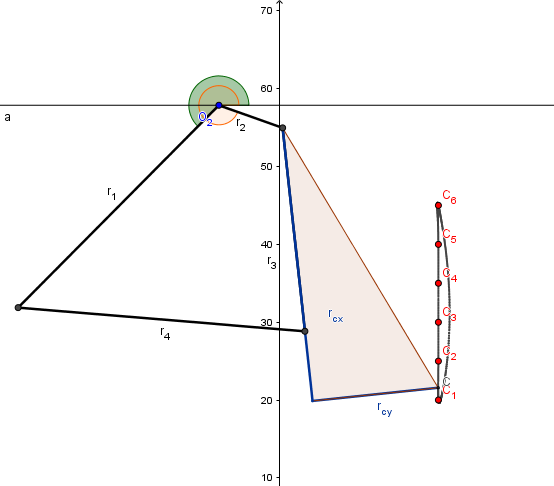
\includegraphics[width=\linewidth]{Figures/MCE1}
		\caption{MCE1} \label{fig:M1} 
	\end{subfigure}\hfill
	\begin{subfigure}[b]{0.49\linewidth}
		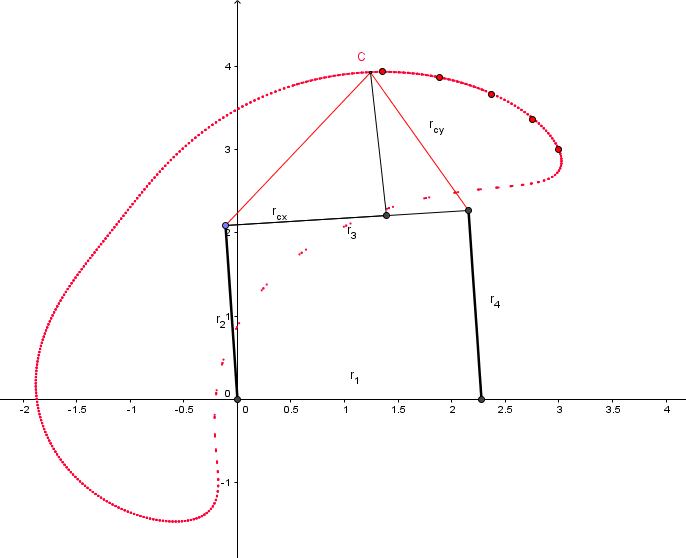
\includegraphics[width=\textwidth]{Figures/MCE2}
		\caption{MCE2} \label{fig:M2} 
	\end{subfigure}
\hfill
\hfill
	\begin{subfigure}[b]{0.49\linewidth}
		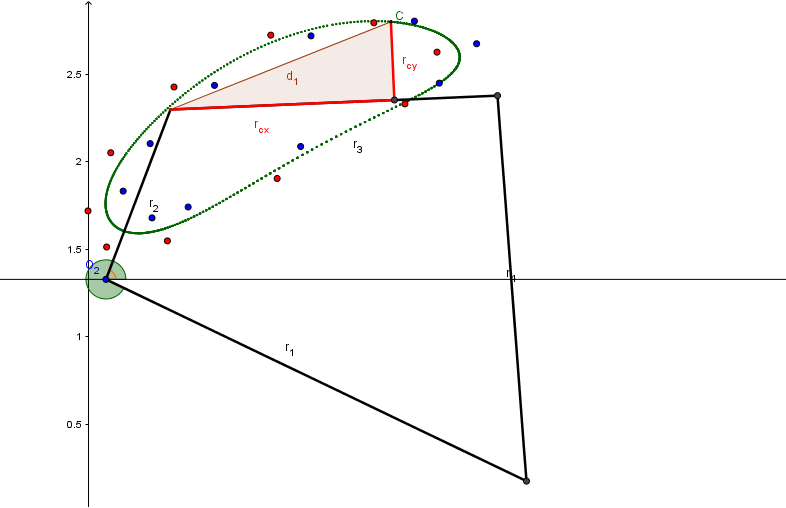
\includegraphics[width=\linewidth]{Figures/MCE3}
		\caption{MCE3} \label{fig:M3} 
	\end{subfigure}
	
	\caption{Mecanismos correspondientes a las mejores soluciones encontradas por el algoritmo HNMED-V6 en los
		tres casos de estudio de la Síntesis Óptima del Mecanismo de Cuatro Barras.} \label{fig: Mecanismos correspondientes a las mejores soluciones encontradas por el algoritmo HNMED-V6 en los
		tres casos de estudio de la Síntesis Óptima del Mecanismo de Cuatro Barras.} 
	
\end{figure}					
%%%%%%%%%%%%%%%%%%%%%%%%%%%%%%%%%%%%%%%%%%%%%%%%%%%%%%%%%%%%%%%%%%%%%%%%%%%%%%%%%
\subsection{Efector Final de Tres Dedos}
Los vectores de diseño obtenidos mediante para los dos casos
de estudio de la Síntesis Óptima del  Efector Final de Tres Dedos se muestran en la Tabla \ref{Vectores de diseño por HNMED-V6 y C-LSHADE para los dos casos de estudio del efector final de tres dedos, correspondientes al la mejor observación de la muestra.} . A partir de estos vectores se realizaron las simulaciones correspondientes cuyas gráficas se presentan en la Figura \ref{fig: Efectores finales  correspondientes a las mejores soluciones encontradas por el algoritmo HNMED-V6 en los dos casos de estudio de la Síntesis Óptima de un Efector Final de Tres Dedos.}. Los resultados encontrados para el caso 1 confirman la multimodalidad del función objetivo de este problema, ya que se obtuvieron vectores diferentes con el mismo valor de $F(\vec{x})$. En la Tabla \ref{Vectores de diseño por HNMED-V6 y C-LSHADE para los dos casos de estudio del efector final de tres dedos, correspondientes al la mejor observación de la muestra.} se muestran en la columna correspondiente a HNMED-V6 dos de las soluciones óptimas encontradas (de izquierda a derecha $\vec{x}_1$ y $\vec{x}_2$). Se puede observar en las subfiguras A) y B) (Figura \ref{fig: Efectores finales  correspondientes a las mejores soluciones encontradas por el algoritmo HNMED-V6 en los dos casos de estudio de la Síntesis Óptima de un Efector Final de Tres Dedos.}) la diferencia entre las longitudes de las barras de ambos efectores que alcanzan el valor de $F(\vec{x})=0$. Es importante destacar que aunque sólo se muestran dos vectores diferentes, en el experimento F por ejemplo, se observaron 11 vectores de diseño diferentes con el valor de $F(\vec{x})=0$. Estos resultados experimentales aportan nuevos conocimientos sobre la naturaleza de estas funciones.

 Además, la multimodalidad permite obtener diferentes soluciones óptimas que proporcionan un espectro más amplio para la toma de decisiones por parte de los diseñadores. En el problema GCE2, se obtiene un mecanismo resultante de aplicar la fórmula de normalización de barras, la cual concibe la estética del mecanismo y logra un diseño más antropomorfo que en GCE1. Esto limita al mecanismo para alcanzar una precisión mayor, a diferencia del caso 1 donde se alcanza la precisión máxima con error igual cero.
\begin{table}
	\centering
	\caption{Vectores de diseño por HNMED-V6 y C-LSHADE para los dos casos de estudio del efector final de tres dedos, correspondientes al la mejor observación de la muestra.} \label{Vectores de diseño por HNMED-V6 y C-LSHADE para los dos casos de estudio del efector final de tres dedos, correspondientes al la mejor observación de la muestra.}
	\begin{tabular}{|c|c|c|c|c|c|} 
		\hline
			\multirow{2}{*}{\textbf{Variables}} & \multicolumn{3}{c|}{\textbf{GCE1}} & \multicolumn{2}{c|}{\textbf{GCE2}}   \\ 
		\cline{2-6}
	                &\multicolumn{2}{c|}{\textbf{HNMED-V6}}&\textbf{ C-LSHADE   }&\textbf{ HNMED-V6    } & \textbf{C-LSHADE     }\\ 
		\hline
		$r_1$        & 32.1665 &75.7315 &93.3515    & 67.3809  & 67.3809      \\ 
		\hline
		$r_2$        & 15.4153  &18.7233& 24.8445    & 26.9523  & 26.9523      \\ 
		\hline
		$r_3$        & 57.3403  &80.6528 &91.1652    & 80.8570  & 80.857       \\ 
		\hline
		$r^1_4$       & -49.9221&-17.3087&-10.7608   & -19.3905 & -8.5852      \\ 
		\hline
		$r^2_4$       & -41.8768  &-31.5388& -26.3809   & -34.0277 & -25.1694     \\ 
		\hline
		$r^3_4$       & -32.2552 &-45.6307 &-41.9142   & -49.6243 & -41.3845     \\ 
		\hline
		$r_0$        & 31.6542  &53.4419&61.6546    & 53.9841  & 53.9841      \\ 
		\hline
		$r'_2$       & 21.5820  &74.4829&117.6764   & 76.3699   & 76.3699      \\ 
		\hline
		$r_5$        & 19.3986  &48.7177 &37.8306    & 50           & 50           \\ 
		\hline
		$r_6$        & 33.1513  &75.4862&128.4622   & 76.3699   & 76.3699      \\ 
		\hline
		$r_{EX}$       & 18.3572  &35.7005& 12.18      & 50           & 50           \\ 
		\hline
		$r_{EY}$       & 149.8560  &90.3028& 52.5227    & 80.8429  & 80.8429      \\ 
		\hline
		$\alpha$     & 0.26237  &0.6646& 0.6639     & 0.5093  & 0.2618       \\ 
		\hline
		$\theta_0$    & 3.2378  &2.6777 &3.0013     & 2.4927  & 2.4927       \\ 
		\hline
	\textbf{	FO   }     & 0     &0       & 0          & 0.11385  & 0.11385  \\
		\hline
	\end{tabular}
\end{table}


\begin{figure}
	\centering
	\begin{subfigure}[b]{0.45\linewidth}
		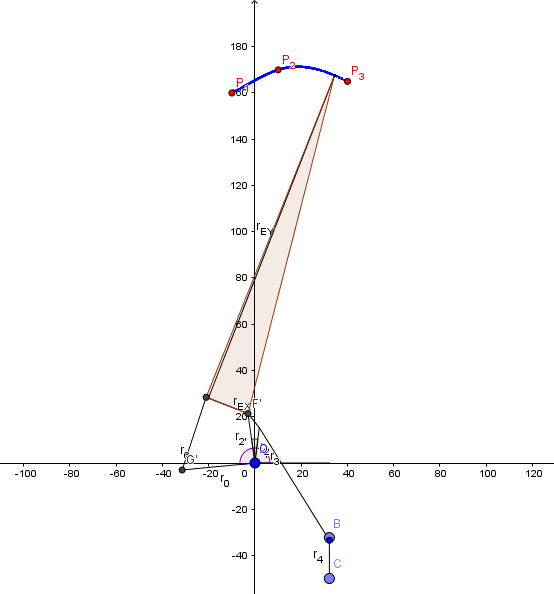
\includegraphics[width=\linewidth]{Figures/GCE1}
		\caption{GCE1 ($\vec{x}_1$)} \label{fig:G1} 
	\end{subfigure}
	\begin{subfigure}[b]{0.45\linewidth}
	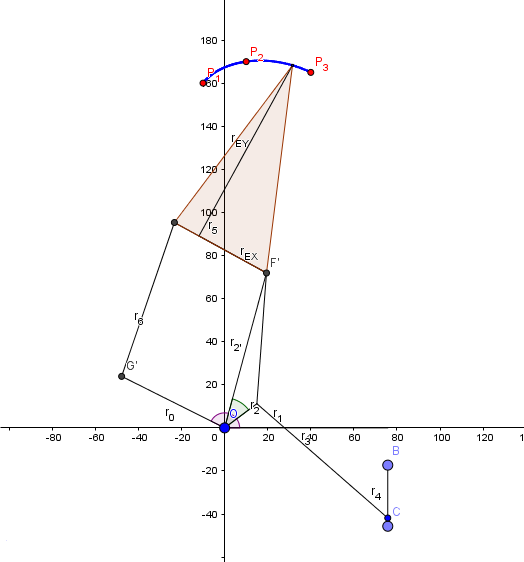
\includegraphics[width=\linewidth]{Figures/GCE1_2}
	\caption{GCE1  ($\vec{x}_2$)} \label{fig:G1} 
\end{subfigure}
	\begin{subfigure}[b]{0.49\linewidth}
		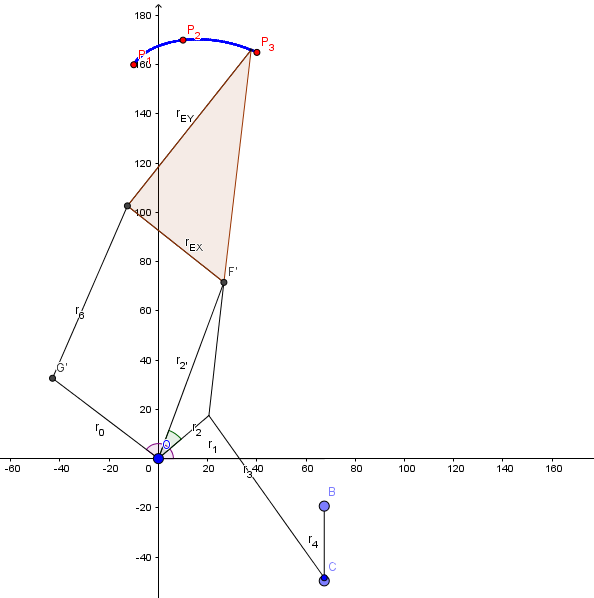
\includegraphics[width=\textwidth]{Figures/GCE2}
		\caption{GCE2} \label{fig:G2} 
	\end{subfigure}
	\caption{Efectores finales  correspondientes a las mejores soluciones encontradas por el algoritmo HNMED-V6 en los
		dos casos de estudio de la Síntesis Óptima de un Efector Final de Tres Dedos.} \label{fig: Efectores finales  correspondientes a las mejores soluciones encontradas por el algoritmo HNMED-V6 en los dos casos de estudio de la Síntesis Óptima de un Efector Final de Tres Dedos.} 
\end{figure}	

\subsection{Microrred Aislada}

En el problema de la Micro-red Eléctrica Aislada se logró minimizar el costo de generación de energía eléctrica durante cada hora del día, alcanzándose un costo total de \textbf{-5.5147E+05}, superior al alcanzado por C-LSHADE, LSHADE-CV y ED/rand/1/bin. El valor negativo significa el ahorro monetario alcanzado, debido a la mayor utilización de las Fuentes de Energía Renovable(FER) durante el despacho en el día.
La Tabla \ref{Vectores de diseño obtenidos por HNMED-V6 para la microrred aislada en las 24 horas del día, correspondientes al la mejor observación de la muestra} se muestra los valores encontrados para las variables de
diseño en cada hora del día. A modo de comparación se agregaron los valores obtenidos por el algoritmo LSHADE-CV el cual obtuvo mejores resultados que C-LSHADE para este problema en \cite{zapata_zapata_control_2017}. Se puede observar que en la hora 12 HNMED-V6 obtiene un mayor ahorro reduciendo la generación mediante diesel y ESS y aumentando la generación por medio de energía solar y eólica respecto a la hora anterior. 

A partir de estos vectores se generó la Figura \ref{Visualización del suministro de energía durante las 24 horas del día para el funcionamiento de la microrred aislada, obtenido por el algoritmo HNMED-V6.} en la que se muestra la potencia que alcanza cada uno de los generadores en respuesta a la demanda (Carga del sistema). Como se puede observar, el sumunistro mediante el Generador de Díesel (P1) tiene la mayor asignación de carga durante las primeras  y últimas horas del día, sin embargo a partir de la hora 12 a la 18, el sumunistro es asumido mayormente por las FER permitiendo alcanzar el un ahorro significativo en comparación con el alcanzado por LSHADE-CV,C-LSHADE y ED/rand/1/bin.

\begin{table}
	\centering
	\caption{Vectores de diseño obtenidos por HNMED-V6 para la microrred aislada en las 24 horas del día, correspondientes al la mejor observación de la muestra}\label{Vectores de diseño obtenidos por HNMED-V6 para la microrred aislada en las 24 horas del día, correspondientes al la mejor observación de la muestra}
	\centering
\resizebox{\textwidth}{!}{%	
	\begin{tabular}{|c|c|c|c|c|c|c|} 
		\hline
	\textbf{	t} &\textbf{ P1(Diesel)         }&\textbf{ P2(ESS)         }& \textbf{P3(Solar)      }&\textbf{ P4 (Eólica)}& \textbf{$FO_t$ (HNMED-V6) }& \textbf{$FO_t$ (LSHADE-CV) } \\ 
		\hline
		0    & 2496.2999  & 1.7        & 1          & 1          & 744.7866      & 744.7866        \\ 
		\hline
		1    & 1755.8416  & 341.2007   & 1.1127E-03 & 402.9565   & -4753.1500    & -6167.8006      \\ 
		\hline
		2    & 1704.1952  & 394.8047   & 0.9999     & 749.9999   & -16558.9336   & -21918.5478     \\ 
		\hline
		3    & 2232.9547  & 116.0452   & 1          & 600        & -18862.8782   & -13517.0085     \\ 
		\hline
		4    & 1964.1355  & 344.2916   & 0.9995     & 540.5732   & -9947.9769    & -15310.5979     \\ 
		\hline
		5    & 1939.3028  & 319.8534   & 0.07404    & 240.7696   & 877.3945      & 6780.1853       \\ 
		\hline
		6    & 1363.3840  & 437.2674   & 0.9937     & 348.3547   & -109.7044     & -2731.4501      \\ 
		\hline
		7    & 1983.9986  & 1.7474E-04 & 265.9997   & 1.4022E-03 & -35662.9968   & -35701.6365     \\ 
		\hline
		8    & 2228.9763  & 2.3807E-02 & 69.9998    & 0.9999     & -8864.0039    & -8864.7210      \\ 
		\hline
		9    & 1786.2962  & 165.0891   & 368.6145   & 6.4863E-10 & -44829.1086   & -30445.4635     \\ 
		\hline
		10   & 2283.5514  & 45.4304    & 21.0178    & 2.2889E-04 & -770.1488     & -16260.0739     \\ 
		\hline
		11   & 1897.9986  & 826.2181   & 125.9999   & 99.7831    & 4142.6902     & -9881.8426      \\ 
		\hline
		12   & 884.9261   & 500.9353   & 692.8439   & 171.2945   & -85880.2563   & -70753.5073     \\ 
		\hline
		13   & 525.7193   & 1098.3992  & 693.2158   & 2.6656     & -61804.5468   & -27202.5115     \\ 
		\hline
		14   & 2.6908E-02 & 1099.7761  & 606.4617   & 643.7351   & -74471.8475   & -85010.2124     \\ 
		\hline
		15   & 210.1557   & 1019.5926  & 559.9858   & 560.2657   & -67319.5302   & -71276.2124     \\ 
		\hline
		16   & 61.6439    & 1040.7287  & 405.8161   & 941.8111   & -60257.4986   & -56471.1139     \\ 
		\hline
		17   & 921.2967   & 1023.9955  & 62.9982    & 1141.7095  & -21515.5577   & -22707.6927     \\ 
		\hline
		18   & 915.8894   & 1099.9959  & 0.9997     & 1293.1147  & -16585.2094   & -16585.2296     \\ 
		\hline
		19   & 2398.1511  & 850.8494   & 0.9993     & 999.9999   & -12168.3814   & -12168.4505     \\ 
		\hline
		20   & 3747.7705  & 1.2300     & 0.9997     & 499.9996   & -17364.3302   & -17399.8776     \\ 
		\hline
		21   & 2409.9582  & 40.0413    & 3.1178E-04 & 550        & -18977.4352   & -19017.7949     \\ 
		\hline
		22   & 2449.4718  & 208.8747   & 1.9987E-02 & 291.6334   & -4075.7627    & -4318.2607      \\ 
		\hline
		23   & 1304.2459  & 1100       & 0.9999     & 244.7540   & 23536.9265    & 23676.9774      \\ 
		\hline
		\multicolumn{5}{|c|}{\textbf{Total}}                              & -5.5147E+05   & -5.3250E+05     \\
		\hline
	\end{tabular}
}
\end{table}

\begin{figure}
	\centering

		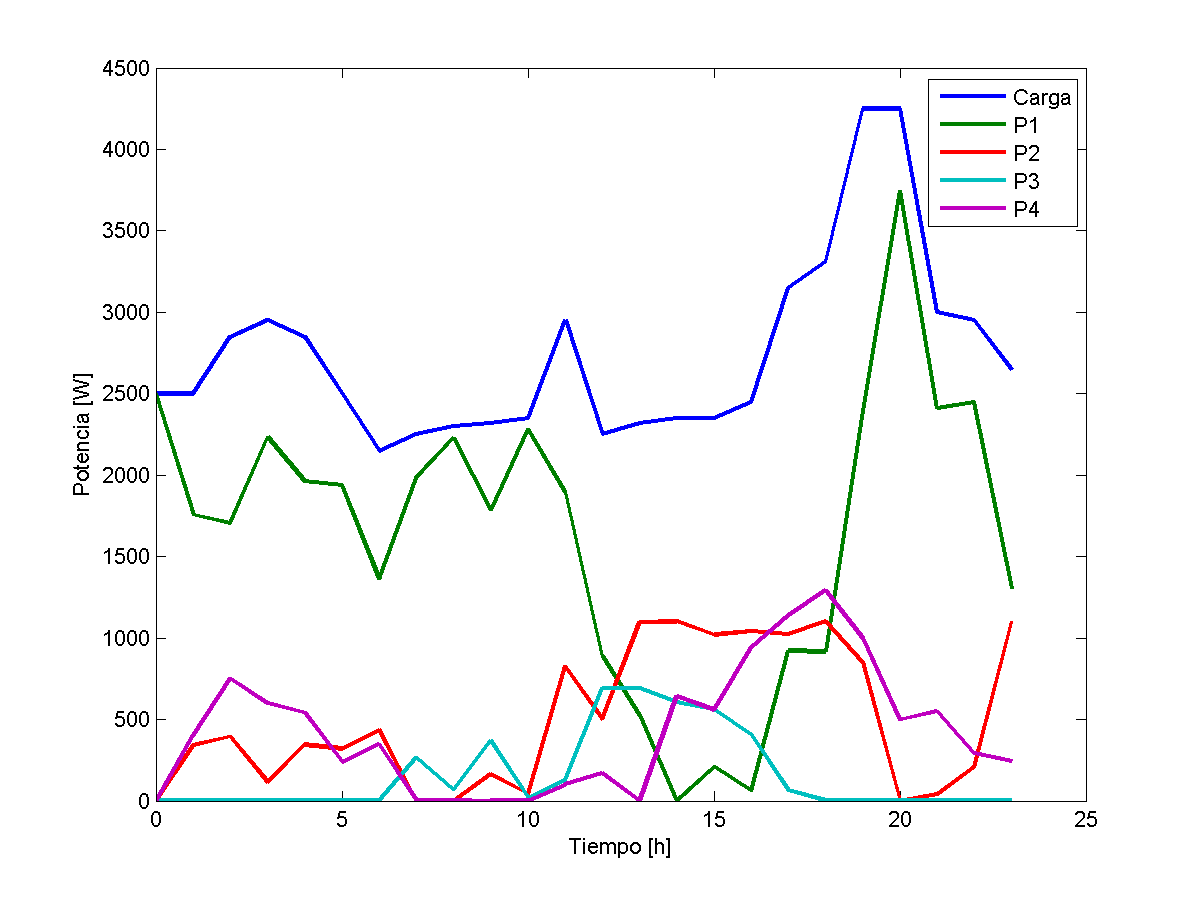
\includegraphics[width=\textwidth]{Figures/SCE1}


	\caption{Visualización del suministro de energía durante las 24 horas del día para el funcionamiento de la microrred aislada, obtenido por el algoritmo HNMED-V6.} \label{Visualización del suministro de energía durante las 24 horas del día para el funcionamiento de la microrred aislada, obtenido por el algoritmo HNMED-V6.}
\end{figure}


\section{Conclusiones del capítulo}
En el presente capítulo se describió el diseño experimental llevado a cabo para diseñar la propuesta de solución. Este proceso de experimentación se llevo a cabo en dos etapas: Una fase de experimentos preliminares que tuvo como objetivo validar la competitividad del enfoque de hibridación propuesto y evaluar el comportamiento de las primeras 5 variantes presentadas. Los resultados obtenidos en experimentos preliminares sirvieron para guiar el diseño del algoritmo HNMED-V6 el cual incluye una estrategia de inicialización de los símpleces y el buscador global se aplica a un subconjunto élite mayor durante el proceso de minimización. Los experimentos finales muestran un desempeño competitivo de esta versión con respecto a los algoritmos ED/rand/1/bin y C-LSHADE. Sin embargo HNMED-V6 utiliza un número inferior de evaluaciones de la función objetivo.